\documentclass[sigconf,10pt,anonymous,review,screen]{acmart}
%%

%% Rights management information.  This information is sent to you
%% when you complete the rights form.  These commands have SAMPLE
%% values in them; it is your responsibility as an author to replace
%% the commands and values with those provided to you when you
%% complete the rights form.
% \setcopyright{acmlicensed}
% \copyrightyear{2018}
% \acmYear{2018}
% \acmDOI{XXXXXXX.XXXXXXX}
%% These commands are for a PROCEEDINGS abstract or paper.
% \acmConference[Conference acronym 'XX]{Make sure to enter the correct
%   conference title from your rights confirmation email}{June 03--05,
%   2018}{Woodstock, NY}
%%
%%  Uncomment \acmBooktitle if the title of the proceedings is different
%%  from ``Proceedings of ...''!
%%
%%\acmBooktitle{Woodstock '18: ACM Symposium on Neural Gaze Detection,
%%  June 03--05, 2018, Woodstock, NY}
% \acmISBN{978-1-4503-XXXX-X/2018/06}


% 
\usepackage{amsmath,amsthm}
%\usepackage{mathtools}
\usepackage{bbm} % For \mathbb{1} (the indicator function)
\usepackage{hyperref}
\usepackage[capitalise]{cleveref}
\usepackage{xcolor}
\usepackage[shortlabels]{enumitem}

%
%\setlength{\marginparwidth}{3.4cm} % TODO: remove this later.
\usepackage{todonotes} % TODO: remove this later.
%
%\renewcommand{\familydefault}{\sfdefault}
%\usepackage{kpfonts}

\title{Duality in Orbit-finite Linear Programming or
Smoothly approximated linear programs}
%
\author{anon.}
%
\date{}
%
% !TEX root = main.tex
%
%\usepackage{amssymb,amsmath,amsthm}
%\usepackage{mathrsfs}
%\usepackage[dvipsnames]{xcolor}
%\usepackage{enumitem}
\usepackage[shortlabels]{enumitem}
\usepackage{hyperref}
\usepackage{cleveref}
%\usepackage[hyperref,amsthm]{ntheorem} %use either this or ntheorem
\usepackage{thmtools}
\addtotheorempostheadhook[thm]{\crefalias{thmlisti}{thm}}
\addtotheorempostheadhook[lem]{\crefalias{thmlisti}{lem}}
%\usepackage{textcomp}
%\usepackage{nicematrix}
\usepackage{blkarray}
\usepackage{tabularx,lipsum,environ}
%\usepackage{ragged2e}
\usepackage{mathrsfs}
%\usepackage{xspace}
\usepackage[normalem]{ulem} % for strikethroughing text using \sout{}
\usepackage{color,soul} %for underlining
\setul{}{1pt}
\usepackage[all]{xy}
\usepackage{tikz}
\usetikzlibrary{arrows.meta,positioning,petri}
\usepackage{algorithm}
\usepackage[noend]{algpseudocode} %for algorithm environment
\usepackage{etoolbox}
\usepackage{chngcntr}
%\usepackage{todonotes}
\usepackage{leftindex}
\usepackage[symbols,nogroupskip,sort=none]{glossaries-extra}

\usepackage{tikz-cd}
\usepackage[nonewpage]{imakeidx}
%\usepackage[numbib,notindex]{tocbibind}

\usepackage{titletoc}
\usepackage[toctitles]{titlesec}

\allowdisplaybreaks

% For having only the figure number in caption
\usepackage{caption}
\DeclareCaptionFormat{empty}{#1}
\renewcommand*\figurename{Figure}
%
%
\newglossary[slg]{symbolslist}{syi}{syg}{List of commonly used symbols}
%
%
%\renewcommand{\emph}[1]{\textcolor{purple}{\textit{#1}}} %to make emphs more noticeable since we use them to define things outside definition environment
%
%\sethlcolor{olive}
\newcommand{\emphdef}[1]{\textcolor{purple}{\emph{#1}}}
\newcommand{\defind}[2]{\emphdef{#1}{\index[terms]{#2}}}
\newcommand{\defindS}[1]{\defind{#1}{#1}}
\newcommand{\defindKey}[2]{\defind{#1}{#2@#1}}
\newcommand{\defindSym}[2]{\emphdef{#1}{\index[symbols]{#2}}}
\newcommand{\defindSymS}[1]{\defindSym{#1}{#1}}
%\newcommand{\emphdef}[1]{\text{\hl{#1}}}
\newcommand{\orbsumlp}[1]{#1^{\Sigma}}
\colorlet{Mycolor1}{red!50!blue}
\newcommand{\indexcolor}[1]{\textcolor{Mycolor1}{#1}}
%
\usepackage[flushmargin,ragged]{footmisc} % this removes indentation from footnotes and makes them left aligned
%
%\usepackage{lineno}
%\linenumbers
\crefname{section}{§}{§§}
\Crefname{section}{§}{§§}
%
%
% Trying to add a line beside proofs
%
%\usepackage[most]{tcolorbox}
%\renewenvironment{proof}[1][Proof]
%{\begin{tcolorbox}[freelance,
%breakable,
%width=\dimexpr\textwidth+28pt\relax,
%before=\par\vspace{\bigskipamount}\noindent,
%colback=white,
%enlarge left by=-14pt,
%%overlay unbroken and first={
%%%  \node[
%%%  anchor=north east,
%%%  inner xsep=8pt,
%%%  xshift=8pt,
%%%  rounded corners=5pt,
%%%  font=\bfseries,
%%%  fill=white] at ([xshift=-0.2cm]frame.north west) (tit) {\strut Example:};
%%  \draw[
%%  line width=3pt,
%%  rounded corners=5pt,gray
%%  ] ([xshift=4pt]frame.north west) -- ([xshift=4pt]frame.south west);
%%},
%%overlay middle and last={
%%  \draw[
%%  line width=3pt,
%%  rounded corners=5pt,gray
%%  ] ([xshift=4pt]frame.north west) -- ([xshift=4pt]frame.south west);
%%},
%frame code={},
%interior code={},
%top=0pt,
%bottom=0pt,
%title=#1,
%borderline west={1pt}{0pt}{black},
%coltitle = black,
%opacityframe=0,
%opacityfill=0]
%}
%{\qed\end{tcolorbox}}
%
%
%%%%%%%%%%%%%%%%%%%%%%   symbols   %%%%%%%%%%%%%%%%%%%%%
%
\renewcommand{\a}{\alpha}
\renewcommand{\b}{\beta}
\newcommand{\g}{\gamma}
\newcommand{\A}{\mathbb{A}}
\newcommand{\cB}{\mathcal{B}}
\newcommand{\cC}{\mathcal{C}}
\newcommand{\N}{\mathbb{N}}
\newcommand{\Q}{\mathbb{Q}}
\newcommand{\Z}{\mathbb{Z}}
\newcommand{\R}{\mathbb{R}}
\newcommand{\F}{\mathbb{F}}
\newcommand{\X}{\mathbb{X}}
\newcommand{\sS}{\mathcal{S}}
\newcommand{\cU}{\mathcal{U}}
\newcommand{\W}{\mathbb{W}}
\newcommand{\id}{\textnormal{Id}}
\newcommand{\ptime}{\textsc{Ptime}}
\newcommand{\dlo}{\mathbb{D}}
\newcommand{\subseteqfin}{\subseteq_{\textsc{fin}}}
\newcommand{\supseteqfin}{\supseteq_{\textsc{fin}}}

\newglossaryentry{symb:fin sub}{
 	name=$\subseteqfin$,
 	description={``is a finite subset of''},
 	sort=subseteqfin,
 	type=symbolslist
}
%
\newglossaryentry{symb:fin sup}{
 	name=$\supseteqfin$,
 	description={``is a finite superset of''},
 	sort=supseteqfin,
 	type=symbolslist
}

\newglossaryentry{symb:disun}{
 	name=$\uplus$,
 	description={disjoint union},
 	sort=disun,
 	type=symbolslist
}

\newglossaryentry{symb:num real}{
 	name=$\R$,
 	description={the set of real numbers},
 	sort=numreal,
 	type=symbolslist
}

\newglossaryentry{symb:num real pos}{
 	name=$\R_+$,
 	description={the set of positive real numbers},
 	sort=numrealpos,
 	type=symbolslist
}

\newglossaryentry{symb:num real nonneg}{
 	name=$\R_{\geqslant 0}$,
 	description={the set of non-negative real numbers},
 	sort=numrealnonneg,
 	type=symbolslist
}

\newglossaryentry{symb:num nat}{
 	name=$\N$,
 	description={the set of natural numbers},
 	sort=num nat,
 	type=symbolslist
}

\newglossaryentry{symb:num int}{
 	name=$\Z$,
 	description={the set of integers},
 	sort=numint,
 	type=symbolslist
}

\newglossaryentry{symb:num int pos}{
 	name=$\Z_+$,
 	description={the set of positive integers},
 	sort=numintpos,
 	type=symbolslist
}
\newcommand{\symgr}[1]{\textnormal{\textbf{S}}_{#1}}
\newglossaryentry{symb:symgr}{
 	name=$\symgr{k}$,
 	description={symmetric group of degree $k$},
 	sort=symgr,
 	type=symbolslist
}



\newcommand{\otufrom}[2]{#1^{(#2)}}
%
\newcommand{\iden}{\textnormal{Id}}
\newcommand{\sE}{\mathcal{E}}
%%%%%%%%%%%%%%%%%%%%%%   macros   %%%%%%%%%%%%%%%%%%%%%

\newcommand{\aut}[2][]{\textnormal{Aut}_{#1}(#2)}
\newcommand{\cone}{\textnormal{cone}}
\newcommand{\col}{\textnormal{col}}
% the extra set of brackets around \left( and \right) is to prevent the extra space given before \left(
\newcommand{\flin}[2][]{\textnormal{FinLin}_{#1}{\left(#2\right)}}
\newcommand{\flinWB}[2][]{\textnormal{FinLin}_{#1}{#2}}
\newcommand{\fsum}[1]{\textnormal{FinSum}{\left(#1\right)}}
\newcommand{\lin}[2][]{\textnormal{Lin}_{#1}{\left(#2\right)}}
\newcommand{\row}{\textnormal{row}}
\newcommand{\set}[1]{\left\{#1\right\}}
\newcommand{\setwith}[1]{\textnormal{Set}#1}
%\newcommand{\setof}[2]{\left\{#1 \ \middle| \ #2\right\}}
\newcommand{\setof}[2]{\left\{#1 \ : \ #2\right\}}
\newcommand{\vr}[1]{\mathbf{#1}}
\newcommand{\transpose}[1]{#1^{\mathsf{T}}}
\newcommand{\supp}[1]{\textnormal{support}\left(#1\right)}
\newcommand{\orbit}[2][]{\textnormal{orbit}_{#1}{(#2)}}
\newcommand{\farkas}{Farkas\textquotesingle{ }}
\newcommand{\defeq}{\overset{\mathrm{def}}{=}}
\newcommand{\defiff}{\overset{\mathrm{def}}{\iff}}
\newcommand{\orbits}[2][]{\textnormal{Orbits}_{#1}{(#2)}}
\newcommand{\orbSum}[1]{\Gamma_{#1}}
\newcommand{\orbsum}[1]{\gamma_{#1}}
\newcommand{\orbdis}[2]{\delta^{#1}_{#2}}
\newcommand{\orbrow}[1]{\delta_{#1}}
\newcommand{\orbsmt}[2]{\gamma^{#1}_{#2}}
\newcommand{\orbres}{\zeta}
\newcommand{\idvec}[1]{\mathbf{1}_{#1}}
\newcommand{\del}[1]{\textnormal{delete}_{#1}}
\newcommand{\otu}[2]{(\A\setminus #1)^{(#2)}}
\newcommand{\otuequiv}[1]{\A^{(#1)}}
\newcommand{\otuquotient}[3]{(\otu{#1}{#2}/_{#3})}
\newcommand{\tuple}[1]{\overline{#1}}
\newcommand{\fadp}{\textsc{FADP}}
\newcommand{\Wlog}{\textsc{WLOG}}
\newcommand{\bit}[1]{\textnormal{bit}(#1)}
\newcommand{\npc}{\textsc{NP}\textnormal{-complete}}

%%%%%%%%%%%% Macros for drawing block matrices %%%%%%

\newcommand{\drawMat}[3]{
\left[
\begin{tabular}{#1}
\color{Mycolor1}#2 \color{black}\\
#3
\end{tabular}
\right]
}
%
%%%%%%%%%%%% Macros for basis %%%%%%
%
\newcommand{\dimm}[2]{#1\textnormal{-dim}{\left(#2\right)}}
\newcommand{\TO}[2]{\textnormal{TO}{\left(#1,#2\right)}}
\newcommand{\odom}[2]{{#1\textnormal{-orbit-dom}{\left(#2\right)}}}
\newcommand{\pair}[4]{\leftindex^{#1}_{#2} O^{#3}_{#4}}
\newcommand{\OaT}{\pair{}{\a}{T}{}}
\newcommand{\ObT}{\pair{}{\b}{T}{}}
\newcommand{\OTa}{\pair{T}{}{}{\a}}
\newcommand{\OTb}{\pair{T}{}{}{\b}}
\newcommand{\OTT}{\pair{T}{}{T}{}}

%
%%%%%%%%%%%% Macros for equations %%%%%%
%
\newcommand{\Span}[2][]{\textsc{Span}_{#1}(#2)} % note the capitalisation
\newcommand{\fSpan}[2][]{\textsc{Fin-Span}_{#1}(#2)}
\newcommand{\fSpanK}[3]{\textsc{Fin-Span}_{#1}^{#2}(#3)}
\newcommand{\np}{\textsc{NP}}
\newcommand{\eq}[1]{\textsc{Eq($#1$)}}
\newcommand{\finEq}[1]{\textsc{Fin-Eq($#1$)}}
\newcommand{\genEq}[1]{\textsc{Gen-Eq($#1$)}}
\newcommand{\equivEq}[1]{\textsc{Support-Preserving-Eq($#1$)}}
\newcommand{\cD}[1]{\mathcal{D}_{#1}}
%
\newcommand{\comp}[2]{#1_#2}
\newcommand{\main}[1]{\widetilde{#1}}
%\newcommand{\ordsolv}{\text{$<$-equivariant solvability}}
\newcommand{\ordprob}[1]{$\textsc{Fin-Eq}_{<}(#1)$}
\newcommand{\ordsolvtext}{order equivariant finitary solvability}
\newcommand{\Ordsolvtext}{Order equivariant finitary solvability}
\newcommand{\ordequiv}{order equivariant}
%
\newcommand{\maindom}[1]{\widetilde{\textnormal{d}}\textnormal{om}(#1)}
\newcommand{\lex}[1][]{<_{\ell\textnormal{ex}}^{#1}}
\newcommand{\lexeq}[1][]{\leqslant_{\ell\textnormal{ex}}^{#1}}
%%%%%%%%%%%% Macros for equivariant subspaces %%%%%%
%
\newcommand{\basis}[2][]{\textsc{Basis}_{#1}{\left(#2\right)}}
\newcommand{\length}[2][]{\textsc{Length}_{#1}{(#2)}}
%
% the brackers around \left( and \right) is to prevent the extra space around them
\newcommand{\dom}[1]{\textnormal{dom}{\left(#1\right)}}
\newcommand{\zerovec}{\vr{0}}
\newcommand{\image}[1]{\textnormal{Im}\left(#1\right)}
\newcommand{\spread}[1]{\widetilde{#1}}
\newcommand{\restr}[1]{\arrowvert_{#1}}
\newcommand{\dimred}[2][]{\textnormal{reduc}^{#1}_{#2}}
%
%%%%%%%%%%%%%%%%%%%%%%   environments   %%%%%%%%%%%%%%%%%%%%%
%
% No indentation after theorems
\makeatletter
\def\@endtheorem{\endtrivlist}
\makeatother

\renewcommand{\qedsymbol}{\ensuremath{\blacksquare}}
\makeatletter
\renewcommand{\paragraph}{%
	\@startsection{paragraph}{4}%
	{\z@}{1ex \@plus 1ex \@minus .2ex}{-1em}%
	{\normalfont\normalsize\bfseries}%
}
\makeatother


\theoremstyle{plain}
\newtheorem{theorem}{Theorem}
\newtheorem{lemma}[theorem]{Lemma}
\newtheorem{assumption}[theorem]{Assumption}
\newtheorem{question}[theorem]{Question}
\newtheorem{claim}{Claim}[theorem]
\newtheorem{observation}[theorem]{Observation}
\newtheorem{corollary}[theorem]{Corollary}
\newtheorem{hypothesis}[theorem]{Hypothesis}
\newtheorem{conjecture}[theorem]{Conjecture}

\Crefname{claim}{Claim}{Claims}

\theoremstyle{definition}
\newtheorem{definition}[theorem]{Definition}
\newtheorem{example}[theorem]{Example}
\AtBeginEnvironment{example}{%
  \pushQED{\qed}
  \renewcommand{\qedsymbol}{$\blacktriangleleft$}%
}
\AtEndEnvironment{example}{\popQED\endexample}
\newtheorem{convention}[theorem]{Convention}
\newtheorem{notation}[theorem]{Notation}
\newtheorem*{problem}{Problem}
\newtheorem{remark}[theorem]{Remark}

\newenvironment{subsecproof}[1]{\subsubsection{#1}\pushQED{\qed}}{\popQED\medskip

}
\newenvironment{secproof}[1]{\subsection{#1}\pushQED{\qed}}{\popQED\medskip

}

\newenvironment{latersecproof}[1]
{%
\renewcommand{\theclaim}{\ref{#1}.\arabic{claim}}%
\begin{secproof}{Proof of \Cref{#1}}%
}
{\end{secproof}}

\newenvironment{latersubsecproof}[1]
{%
	\renewcommand{\theclaim}{\ref{#1}.\arabic{claim}}%
	\begin{subsecproof}{Proof of \Cref{#1}}%
	}
{\end{subsecproof}}

%\Crefname{theorem}{Theorem}{Theorems}
%\Crefname{thmenumi}{Theorem}{Theorems}
%\AtBeginEnvironment{theorem}{%
%    \crefalias{enumi}{thmenumi}%
%    \setlist[enumerate,1]{
%        label={\textit{(\roman*)}},
%        ref={\thetheorem.(\roman*)}
%    }%
%}
%
%\Crefname{lemma}{Lemma}{Lemmas}
%\Crefname{lemmaenumi}{Lemma}{Lemmas}
%\AtBeginEnvironment{lemma}{%
%    \crefalias{enumi}{lemmaenumi}%
%    \setlist[enumerate,1]{
%        label={\textit{(\roman*)}},
%        ref={\thelemma.(\roman*)}
%    }%
%}

% IMPORTANT NOTES
%
% 1. Use \newline instead of \\ inside environment
% 2. Put \label inside the second argument
%
%\newcommand{\prob}[4]
%{\begin{problem}[\textsc{#1}]#2
%     $ $\newline
%     \begin{tabularx}{\textwidth}{l  l}
%       \textbf{Input:} & #3 \\
%       \textbf{Question:} & #4 \\
%     \end{tabularx}
% \end{problem}}

\newcommand{\probBasic}[4]
{
\begin{flalign*}
\quad
\begin{tabular}{l  l}
  \multicolumn{2}{l}{\textsc{#1}}\\
  \textbf{Input:}    & #2 \\
  \textbf{#4} & #3
\end{tabular}
&&
\end{flalign*}
}

\newcommand{\prob}[3]
{
\probBasic{#1}{#2}{#3}{Question:}
}

\newcommand{\probOut}[3]
{
\probBasic{#1}{#2}{#3}{Output:}
}
%
\newcommand{\claimQED}{\square}
\newenvironment{claimproof}[1][\proofname]
{\renewcommand\qedsymbol{$\claimQED$}\proof[#1]}
{\endproof}
%\newenvironment{claimproof}{\paragraph{\textnormal{Proof:}}}{
%\smallskip
%
%\hfill $\square$
%\medskip
%
%}
%%%%%%%%%%%%%%%%%   new macros for inequalities  %%%%%%%%%%%%%%%%

\newcommand{\ineq}[1]{\textsc{Ineq($#1$)}}
\newcommand{\finIneq}[1]{\textsc{Fin-Ineq($#1$)}}
\newcommand{\nNEq}[1]{\textsc{Nonneg-Eq($#1$)}}
\newcommand{\finNNEq}[1]{\textsc{Fin-Nonneg-Eq($#1$)}}
\newcommand{\polyineq}{\textsc{Poly-Ineq}}
\newcommand{\allpolyopt}{\textsc{All-Poly-Opt}}
\newcommand{\allpolyineq}{\textsc{All-Poly-Ineq}}

\newcommand{\headPar}[2]{\textnormal{\textsc{head}}_{#2}(#1)}
\newcommand{\head}[1]{\headPar{#1}{}}
\newcommand{\strictHead}[1]{\headPar{#1}{>}}
\newcommand{\tail}[1]{\textsc{tail}(#1)}
\newcommand{\ineqSize}[1]{|#1|}
\newcommand{\G}{\Gamma}
\newcommand{\conj}{\cup}
\newcommand{\ineqal}{\mathcal{E}}
\newcommand{\aasol}{almost-all-solution}
\newcommand{\proj}[1]{\Pi_{#1}}
\newcommand{\orbval}[1]{\dot{#1}}
\newcommand{\exptime}{\textsc{ExpTime}}
\newcommand{\nexptime}{\textsc{NExpTime}}
\newcommand{\twoExptime}{\textsc{2ExpTime}}
\newcommand{\acker}{\textsc{Ackermann}}

%%%%%%%%%%%%%%%%%%%%%%   new macros for LP  %%%%%%%%%%%%%%%%%%%%%

\newcommand{\linProg}{\textsc{Lin-Prog}}

\newcommand{\flinProg}{\textsc{FinLin-Prog}}

\newcommand{\lpMax}[2]
{
\begin{tabular}{l l}
\textnormal{maximise}   & #1\\
\textnormal{subject to} & #2
\end{tabular}
}

\newcommand{\lpMaxMin}[2]
{
\begin{tabular}{r l}
\textnormal{maximise/minimise}   & #1\\
\textnormal{subject to} & #2
\end{tabular}
}


\newcommand{\lpMin}[2]
{
\begin{tabular}{l l}
\textnormal{minimise}   & #1\\
\textnormal{subject to} & #2
\end{tabular}
}

%\lpMaxGen{A}{b}{c}{x}{C}
\newcommand{\lpMaxGen}[5]{
\lpMax{$\transpose{#3}\cdot #4$}{
  $#1 \cdot #4 \leqslant #2$ \\
& $#4\in\lin{#5}$
}}

%\lpMinGen{A}{b}{c}{x}{C}
\newcommand{\lpMinGen}[5]{
\lpMin{$\transpose{#3}\cdot #4$}{
  $#1 \cdot #4 \geqslant #2$ \\
& $#4\in\lin{#5}$ 
}}

\newcommand{\maxGenAbc}{
\lpMaxGen{\vr{A}}{\vr{b}}{\vr{c}}{\vr{x}}{C}
}
%
\newcommand{\minGenAbc}{
\lpMinGen{\vr{A}}{\vr{b}}{\vr{c}}{\vr{x}}{C}
}

\newcommand{\lpMaxFinGen}[5]{
\lpMax{$\transpose{#3}\cdot #4$}{
  $#1 \cdot #4 \leqslant #2$ \\
& $#4\in\flin{#5}$ 
}
}

\newcommand{\lpMinFinGen}[5]{
\lpMin{$\transpose{#3}\cdot #4$}{
  $#1 \cdot #4 \geqslant #2$ \\
& $#4\in\flin{#5}$ 
}
}

\newcommand{\maxFinGenAbc}{
\lpMaxFinGen{\vr{A}}{\vr{b}}{\vr{c}}{\vr{x}}{C}
}

\newcommand{\minFinGenAbc}{
\lpMinFinGen{\vr{A}}{\vr{b}}{\vr{c}}{\vr{x}}{C}
}


%\lpMaxFin{A}{b}{c}{x}{B}{C}
\newcommand{\lpMaxFin}[6]{
\lpMax{$\transpose{#3}\cdot #4$}{
  $#1 \cdot #4 \leqslant #2$ \\
& $#4 \geqslant \vr{0}$ \\
& $#4\in\flin{#6}$ 
}}

%\lpMinFinStan{A}{b}{c}{x}{B}{C}
\newcommand{\lpMinFin}[6]{
\lpMin{$\transpose{#3}\cdot #4$}{
  $#1 \cdot #4 \geqslant #2$ \\
& $#4 \geqslant \vr{0}$ \\
& $#4\in\flin{#6}$ 
}}

\newcommand{\maxFinAbc}{
\lpMaxFin{\vr{A}}{\vr{b}}{\vr{c}}{\vr{x}}{B}{C}
}

\newcommand{\minFinAbc}{
\lpMinFin{\vr{A}}{\vr{b}}{\vr{c}}{\vr{x}}{B}{C}
}

%\lpMatPrimal{A}{b}{c}{x}{B}{C}
\newcommand{\lpMatPrimal}[6]{
\lpMax{$\transpose{#3}\cdot #4$}{
  $#1 \cdot #4 \leqslant #2$ \\
& $#4 \geqslant \vr{0}$ \\
& $#4\in\lin{#6}$ 
}}

%\lpMinPrimal{A}{b}{c}{x}{B}{C}
\newcommand{\lpMinPrimal}[6]{
\lpMin{$\transpose{#3}\cdot #4$}{
  $#1 \cdot #4 \geqslant #2$ \\
& $#4 \geqslant \vr{0}$ \\
& $#4\in\lin{#6}$ 
}}

%\lpMatDual{A}{b}{c}{x}{B}{C}
\newcommand{\lpMatDual}[6]{
\lpMin{$\transpose{#2}\cdot #4$}{
  $\transpose{#1} \cdot #4 \geqslant #3$ \\
& $#4 \geqslant \vr{0}$ \\
& $#4\in\lin{#5}$ 
}}

\newcommand{\primalAbc}{\lpMatPrimal{\vr{A}}{\vr{b}}{\vr{c}}{\vr{x}}{B}{C}}
\newcommand{\minPrimalAbc}{\lpMinPrimal{\vr{A}}{\vr{b}}{\vr{c}}{\vr{x}}{B}{C}}
\newcommand{\dualAbc}{\lpMatDual{\vr{A}}{\vr{b}}{\vr{c}}{\vr{y}}{B}{C}}

%%%%%%%%%%%%%%   macros for column(row)-finite linear programs  %%%%%%%%%%%%%%%

\newcommand{\colLinProg}{\textsc{Col-Fin-Lin-Prog}}

\newcommand{\rowLinProg}{\textsc{Row-Fin-Lin-Prog}}

\newcommand{\colFinMax}[3]{
\begin{tabular}{l l}
\textnormal{Find a vector}  & #1 \\
\textnormal{that maximises} & #2 \\
\textnormal{subject to}     & #3
\end{tabular}
}

\newcommand{\colFinMaxAbc}{
\primalAbc
}

\newcommand{\colFinMinAbc}{
\lpMin{$\transpose{\vr{c}}\cdot \vr{x}$}{
  $\vr{A} \cdot \vr{x} \geqslant \vr{b}$ \\
& $\vr{x}\geqslant\vr{0}$                     \\  
& $\vr{x}\in\lin{C}$
}
}

\newcommand{\rowFinMinAbc}{
\dualAbc 
}

\newcommand{\rowFinMaxAbc}{
\lpMax{$\transpose{\vr{b}}\cdot \vr{y}$}{
  $\transpose{\vr{A}} \cdot \vr{y} \leqslant \vr{c}$ \\
& $\vr{y} \geqslant \vr{0}$ \\
& $\vr{y} : B\to\R$ 
}}

%%%%%%%%%%%%%%%%%%%%%%   comments   %%%%%%%%%%%%%%%%%%%%%

\newcounter{comment}
\setcounter{comment}{1}
\newcommand{\arka}[1]{\noindent\textnormal{\textcolor{red}{\textbf{Arka[\thecomment]:} #1}}\addtocounter{comment}{1}\noindent}
\newcommand{\slawek}[1]{\textnormal{\textcolor{magenta}{\textbf{S\l awek:} #1}}}
\newcommand{\piotrek}[1]{\textnormal{\textcolor{blue}{\textbf{Piotrek[\thecomment]:} #1}}\addtocounter{comment}{1}\noindent}

%%%%%%%%%%%%%%%%%%% For underlining %%%%%%%%%%%%%%%%%%%%%%%%%%%%
%\newcommand{\fixed}[1]{\setulcolor{violet}\ul{#1}\setulcolor{black}}
%\newcommand{\fixed}[1]{\setulcolor{violet}\ul{#1}\setulcolor{black}}
%\newcommand{\fixed}[1]{\textbf{#1}}
\colorlet{fixedcolor}{blue!70!black}
\newcommand{\fixed}[1]{\textcolor{fixedcolor}{#1}}
%%%%%%%%%%%%%%%% Alignment command(s) %%%%%%%%%%%%%%%

% The code below is to make the text left aligned,
% ensuring indententation of paragraphs
\makeatletter
\newcommand\iraggedright{%
  \let\\\@centercr\@rightskip\@flushglue \rightskip\@rightskip
  \leftskip\z@skip}
\makeatother
%

%
% Comment out the four lines below to see the proofs
%\usepackage{environ}
%\NewEnviron{killcontents}{}
%\let\proof\killcontents
%\let\endproof\endkillcontents
%
%\theoremstyle{theorem}
%\newtheorem{theorem}{Theorem}


%\theoremstyle{acmdefinition}
%\newtheorem{remark}[theorem]{Remark}
%\newtheorem{notation}[theorem]{Notation}
%\newtheorem{fact}[theorem]{Fact}
%\theoremstyle{acmplain}
%\newtheorem{claim}[theorem]{Claim}
%
\begin{document}
%
\begin{abstract}
Weal duality holds for oligomorphic.
Strong between column-finite and row-finite holds if and only if smoothly approximated.
We solve both column-finite and row-finite for smoothly approximated.
\end{abstract}
%
\maketitle
%
%!TEX root = main.tex
%
\section{Homogenous structures}\label{sec:hom}
%
\begin{definition}\label{def:rel str}
\arka{Write definition of a countable relational structure.}
\end{definition}
%
\begin{example}\label{eg:eq atom}
\arka{Define equality atoms/domain $\A$.}
\end{example}
%
\begin{example}\label{eg:ord atom}
\arka{Define ordered atoms/domain $\dloQ$}
\end{example}
%
\begin{definition}\label{def:aut}
\arka{Write definition of automorphism group and orbits}
\end{definition}
%
\begin{example}
\arka{Illustrate \Cref{def:aut}}
\end{example}
%
\begin{definition}\label{def:homg}
\arka{Write definition of homogenous relational structure.}
\end{definition}
%
\begin{example}\label{eg:int atom}
\arka{Define integer atoms/domain $\Z = (Z,<)$ to give example of a structure that is not homogenous}
\end{example}
%
\begin{definition}\label{def:oligo}
\arka{Write definition of oligomorphicity.}
\end{definition}
%
\begin{remark}
Homogenous structures with finitely many relations are also oligomorphic \arka{add citation}.
However, the same is not true when there are infinitely many relations.
For example, one can define the structure $\Z' = (Z,D_1,D_2,\dots)$ where $D_n(a,b)$ is true if and only if $x - y = n$.
The structure $\Z'$ is homogenous.
However, it is not oligomorphic as each of the relations $D_n \subseteq Z^2$ forms disjoint orbit
\end{remark}
%
Throughout the article we use $\str = (X,R_1,R_2,\dots)$ to denote an arbitrary countable homogenous relational structure whose automorphism group is oligomorphic.
We use $\str^n$ to denote the set $X^n$.
%
\begin{definition}\label{def:fin supp orb}
\arka{Write definition of finitely supported orbits, and of orbit-finiteness}
\end{definition}
%
\begin{remark}
\arka{orbit-finite subsets of $\str^n$ are exactly the definable ones}
\end{remark}
%
\begin{theorem}
If $\str$ is oligomorphic then $\str^n$ is orbit-finite under the action of $\aut[S]{\str}$ for every $S\subseteqfin \str$.
\end{theorem}
%
\begin{definition}\label{def:ord prop}
The structure $\str$ is said to have the \emphdef{order property} if there is an orbit-finite relation $R\subseteq (\str^n \times \str^n)$ and an infinite subset $D \subseteq \str^n$ such that $R$ defines a linear order on $D$.
\end{definition}
%
\begin{example}
\arka{Illustrate \Cref{def:ord prop}}.

\arka{Example where $n\neq 1$?}
\end{example}
%
For a finite subset $S\subseteq \str$ we use \emphdef{$\subst{S}{\str}$} to denote the relational structure $(S,R_1,R_2,\dots)$.
The notions of homogeneity, automorphism group and orbits extend to $\subst{S}{\str}$ as well.
%
\begin{definition}\label{def:smooth}
The structure $\str$ is said to be \emphdef{smoothly approximated} if there is a chain $S_0 \subseteq S_1 \subseteq S_2 \subseteq \dots$ of subsets of $\str$ such that $\bigcup_{n\in\N} S_n = X$ and $\subst{S_n}{\str}$ is homogenous for every $n$.
\end{definition}
%
\arka{add citation to above def}
%
\begin{example}
\arka{Write which of the structures mentioned before are smoothly approximated and which are not.}
\end{example}
%
\begin{example}
\arka{Bit vector atoms}
\end{example}
%
\begin{example}
\arka{Nestings of smoothly approximated structures are also smoothly approximated.}
\end{example}
%
\begin{theorem}\label{thm:smooth iff}
The structure $\str$ is smoothly approximated if and only if it does not have the order property.
\end{theorem}
%
\begin{proof}
\arka{TODO}
\end{proof}
%
%!TEX root = main.tex
%
\section{Orbit-finite sets}
%
\section{Orbit-finite vectors}\label{sec:ofvec}
%
\section{Orbit-finite matrices}\label{sec:ofmat}
%
\begin{lemma}\label{A b c lemmas}
For any matrix $\vr{A}\in\lin[R]{B{\times}C}$,
$S\subseteqfin \A$ supporting $B$ and $C$ and $\vr{A}$,
$\pi\in\aut[S]{\A}$,
$b\in B$ and $c\in C$:
%
\begin{enumerate}[(i),ref =\Cref{A b c lemmas}-\roman*]
%
\item $\pi(\vr{A}(b,-)) = \vr{A}(\pi(b),-)$ and $\pi(\vr{A}(-,c)) = \vr{A}(-,\pi(c))$.
%
\label{lem:perm mat row}
%
\item
$\supp{\vr{A}(b,-)}\subseteq\supp{\vr{A}}\cup\supp{b}$ and \\
$\supp{\vr{A}(-,c)}\subseteq\supp{\vr{A}}\cup\supp{c}$.
%
\label{lem:row col supp}
%
\end{enumerate}
\end{lemma}
%
\section{Orbit-finite linear programming}\label{sec:hom}
%
\arka{Basic definition and examples}

\arka{Maybe the structure should be: first homogenous structures, then vector spaces, linear programming and duality, then smooth approximation and order property,
and in the end theorems}


%!TEX root = ../../thesis_main.tex
%
% The code below is used to hide the proofs 
%\usepackage{environ}
%\NewEnviron{killcontents}{}
%\let\proof\killcontents
%\let\endproof\endkillcontents
%\let\claimproof\killcontents
%\let\endclaimproof\endkillcontents
%%
%
%
\chapter{Duality in Linear Programming}\label{ch:duality}
%
\minitoc
%
\subsubsection*{Acknowledgements}
%
We are indebted to Damian Niwi\'{n}ski for posing the questions about duality in orbit-finite linear programming.
%
\section{Introduction}
%
For orbit-finite sets $B$ and $C$,
and an orbit-finite $(B\times C)$-linear program
\begin{equation}\label{eq:primal gen}
\primalAbc
\end{equation}
called the \emphdef{primal},
its \emphdef{dual} is defined to be the following $(C\times B)$-orbit-finite linear program
\begin{equation}\label{eq:dual gen}
\dualAbc
\end{equation}
Every such pair \eqref{eq:primal gen}-\eqref{eq:dual gen} of linear programs is known as a \emphdef{primal-dual pair}.
Duals of finite linear programs are clearly finite themselves.
The \emph{weak duality theorem} states that the optimum of every finite linear program is dominated by the optimum of its dual.
The \emph{strong duality theorem} states that for every primal-dual pair of finite linear programs, if the optimum of one of the linear programs is finite, then the optimum of the other linear program is also finite and they are equal.
In this chapter we investigate whether these duality theorems can be extended to the orbit-finite setting. 
%
\vspace{-15pt}
\begin{hypothesis}[Weak Orbit-finite Duality]\label{hypo:weak duality}
For any primal-dual pair of orbit-finite linear programs,
the optimum of the primal is dominated by the optimum of the dual.
\end{hypothesis}
%
\begin{hypothesis}[Strong Orbit-finite Duality]\label{hypo:strong duality}
For any primal-dual pair of orbit-finite linear programs,
if the optimum of one of the linear programs is finite,
then the optimum of the other linear program is also finite and they are equal.
%to each other.
\end{hypothesis}
%
We argue that Hypothesis \ref{hypo:weak duality} is true and Hypothesis \ref{hypo:strong duality} is false.
That is, weak duality holds for orbit-finite linear programs and strong duality does not.
However, both weak and strong duality hold between two natural variations of orbit-finite linear programs,
respectively called \emph{column-finite} and \emph{row-finite} linear programs.

This chapter is divided into five sections.
In Section \ref{sec:weak o.f. duality} we prove Hypothesis \ref{hypo:weak duality}.
In Section \ref{sec:lost} we disprove Hypothesis \ref{hypo:strong duality} by constructing a counterexample.
At the end of Section \ref{sec:lost}, we refine Hypothesis \ref{hypo:strong duality} to pose a conjecture.
In Section \ref{sec:regained} we define column-finite and row-finite linear programming and prove duality between them (Theorem \ref{thm:col row duality}).
\arka{Add other sections}
%Using the results of two latter sections we quickly discuss extensions of asymmetric version of the duality theorems and of Farkas' Lemma respectively in Section \ref{sec:asym} and Section \ref{sec:farkas}.
%
%\arka{The things mentioned in the last sentence are not done}
%
%
\section{Weak duality}\label{sec:weak o.f. duality}
%
In this section we prove Hypothesis \ref{hypo:weak duality},
so it becomes a theorem.
%
\begin{theorem}[Weak Orbit-finite Duality]\label{thm:weak o.f. duality}
The optimum of any orbit-finite linear program is dominated by the optimum of its dual.
\end{theorem}
%
\subsection*{Proof of Theorem \ref{thm:weak o.f. duality}}
%
Let $B$ and $C$ be two arbitrary orbit-finite sets.
Consider a primal-dual pair of orbit-finite linear programs
\[
\primalAbc \quad\quad\quad \dualAbc
\]
where $\vr{A}\in\lin{B\times C}$, $\vr{b}\in\lin{B}$ and $\vr{c}\in\lin{C}$.
To prove that the optimum of the primal is dominated by the optimum of the dual,
it is sufficient to show that for any pair of vectors
${(\vr{x},\vr{y})\in \lin{B} \times \lin{C}}$ such that:
\begin{enumerate}
\item $\vr{x}\geqslant\vr{0}$ and $\vr{y}\geqslant\vr{0}$,
\item the products $\transpose{\vr{c}}\cdot\vr{x}$, $\vr{A}\cdot\vr{x}$,
                   $\transpose{\vr{b}}\cdot\vr{y}$ and
                   $\transpose{\vr{A}}\cdot\vr{y}$ are all well defined, and
\item $\vr{A}\cdot\vr{x} \leqslant \vr{b}$ and
      $\transpose{\vr{A}}\cdot\vr{y} \geqslant \vr{c}$,           
\end{enumerate}
we have $\transpose{\vr{c}}\cdot\vr{x}\leqslant \transpose{\vr{b}}\cdot\vr{y}$.
Fix such a pair of vectors ${(\vr{x},\vr{y})\in \lin{C}\times\lin{B}}$.
If both the products
$\transpose{\vr{y}}\cdot(\vr{A}\cdot\vr{x})$ and
$(\transpose{\vr{y}}\cdot\vr{A})\cdot\vr{x}$ were well-defined then Lemma \ref{lem:orbit-finite assoc} would say that they are equal.
In this case,
we can replicate the proof of weak duality for finite linear programs
(\cite[Page 435]{strang2005}) and conclude
\begin{equation}\label{eq:weak duality proof}
           \transpose{\vr{c}}\cdot \vr{x}
\leqslant (\transpose{\vr{y}}\cdot \vr{A})\cdot\vr{x}
=          \transpose{\vr{y}}\cdot(\vr{A} \cdot\vr{x})
\leqslant  \transpose{\vr{y}}\cdot\vr{b} \ .
\end{equation}
Unfortunately, the products
$\transpose{\vr{y}}\cdot(\vr{A}\cdot\vr{x})$ and
$(\transpose{\vr{y}}\cdot\vr{A})\cdot\vr{x}$ may not be well-defined even in very simple cases
(for example, consider $B = C = \A$, $\vr{A} = \iden_{\A}$, $\vr{b} = \vr{c} = \zerovec$ and $\vr{x} = \vr{y} = \idvec{\A}$).
So we need to be more careful.

The matrix $\vr{A}$ and the vectors $\vr{b}$, $\vr{c}$, $\vr{x}$ and $\vr{y}$ are all finitely supported.
Let $S\subseteq \A$ be the union of their supports
\[
S = \supp{\vr{A}}\cup\supp{\vr{b}}\cup\supp{\vr{c}}
\cup\supp{\vr{x}}\cup\supp{\vr{y}} \ .
\]
Then, $S$ supports all of $\vr{A}$, $\vr{b}$, $\vr{c}$, $\vr{x}$ and $\vr{y}$.
Let $B_S\subseteq B$ and $C_S\subseteq C$ be the subsets of elements of respectively $B$ and $C$ which are supported by $S$
\[
B_S = \setof{b\in B}{\supp{b}\subseteq S}\quad\quad
C_S = \setof{c\in C}{\supp{c}\subseteq S}
\]
\ref{lem:supp aut T} says that $B_S$ and $C_S$ are both finite.
Let $\vr{A}_S\in\lin{B_S\times C_S}$, $\vr{b}_S\in\lin{B_S}$, $\vr{c}_S\in\lin{C_S}$, $\vr{x}_S\in\lin{C_S}$ and $\vr{y}_S\in\lin{B_S}$ be the respective restrictions of
$\vr{A}$, $\vr{b}$, $\vr{c}$, $\vr{x}$ and $\vr{y}$.
Lemma \ref{lem:inner product fin} implies
\begin{equation}\label{eq:finite approx of obj}
\transpose{\vr{c}}  \cdot\vr{x} =
\transpose{\vr{c}_S}\cdot\vr{x}_S
\quad\text{and}\quad
\transpose{\vr{b}}  \cdot\vr{y} =
\transpose{\vr{b}_S}\cdot\vr{y}_S
\end{equation}
Hence, it is enough to show
$\transpose{\vr{c}_S}\cdot\vr{x}_S\leqslant\transpose{\vr{b}_S}\cdot\vr{y}_S$.
This will follow from the next two claims.
\begin{claim}\label{clm:A x b S}
$\vr{A}_S \cdot \vr{x}_S \leqslant \vr{b}_s$
\end{claim}
\begin{claim}\label{clm:A y c S}
$\transpose{\vr{A}_S} \cdot \vr{y}_S \geqslant \vr{c}_s$
\end{claim}
%
\noindent
Before giving the proofs we show how these claims imply 
$\transpose{\vr{c}_S}\cdot\vr{x}_S\leqslant\transpose{\vr{b}_S}\cdot\vr{y}_S$.
The vectors $\vr{x}$ and $\vr{y}$ are both non-negative.
Hence, their restrictions $\vr{x}_S$ and $\vr{y}_S$ are also non-negative.
The matrix $\vr{A}_S$ and the vectors $\vr{b}_S$, $\vr{c}_S$, $\vr{x}_S$ and $\vr{y}_S$ are all finite dimensional.
Hence, the products $ \transpose{\vr{c}_S}\cdot \vr{x}_S$, $(\transpose{\vr{y}_S}\cdot \vr{A}_S)\cdot\vr{x}_S$, $\transpose{\vr{y}_S}\cdot(\vr{A}_S \cdot\vr{x}_S)$ and $ \transpose{\vr{y}_S}\cdot\vr{b}_S$ are all well-defined.
Using non-negativity of $\vr{x}_S$ and $\vr{y}_S$, and Claims \ref{clm:A x b S} and \ref{clm:A y c S} we conclude
\[
               \transpose{\vr{c}_S}\cdot \vr{x}_S
\leqslant (\transpose{\vr{y}_S}\cdot \vr{A}_S)\cdot\vr{x}_S
            =  \transpose{\vr{y}_S}\cdot(\vr{A}_S \cdot\vr{x}_S)
\leqslant  \transpose{\vr{y}_S}\cdot\vr{b}_S \ .
\]
%
\noindent
Now we prove the claims.
The proof of the two claims are similar,
so we concentrate on the first claim only.
%
\begin{proof}[Proof of Claim \ref{clm:A x b S}]
Pick arbitrary $b\in B_S$.
We show
\begin{equation}\label{eq:clm:A x b S 1}
(\vr{A}_S\cdot\vr{x}_S)(b) \leqslant \vr{b}_S(b)
\end{equation}
Since $\vr{b}_S$ is a restriction of $\vr{b}$,
\begin{equation}\label{eq:clm:A x b S 2}
\vr{b}_S(b) = \vr{b}(b)
\end{equation}
The vector $\vr{x}$ satisfies $\vr{A}\cdot\vr{x}\leqslant\vr{b}$.
Hence,
\begin{equation}\label{eq:clm:A x b S 3}
(\vr{A}\cdot\vr{x})(b) \leqslant \vr{b}(b)
\end{equation}
By definition of matrix multplication
\begin{equation}\label{eq:clm:A x b S 4}
(\vr{A}\cdot\vr{x})(b) = \vr{A}(b,-)\cdot\vr{x}
\end{equation}
The set $S$ supports both $b$ and $\vr{A}$.
Lemma \ref{lem:row col supp} implies that $S$ supports the row vector $\vr{A}(b,-)$ as well.
Using Lemma \ref{lem:inner product fin} we can write
\begin{equation}\label{eq:clm:A x b S 5}
 \vr{A}(b,-)\cdot\vr{x} = \sum_{c\in C_S} \vr{A}(b,c)\cdot\vr{x}(c)
 = \vr{A}_S(b,-)\cdot\vr{x}_S
\end{equation}
and by definition $\vr{A}_S$ and $\vr{x}_S$ we can rewrite the latter term as
\begin{equation}\label{eq:clm:A x b S 6}
\vr{A}_S(b,-)\cdot\vr{x}_S
= (\vr{A}_S\cdot\vr{x}_S)(b)
\end{equation}
We get \eqref{eq:clm:A x b S 1} as a consequence of
\eqref{eq:clm:A x b S 2}-\eqref{eq:clm:A x b S 6}
\end{proof}
%
\section{Counterexample to strong duality}\label{sec:lost}
%
In this section we falsify Hypothesis \ref{hypo:strong duality} by giving a counterexample.
We construct a primal-dual pair of orbit-finite linear programs such that the optimum of the primal system is finite but the optimum of the dual system is not.
Let $B = C = \A\uplus\{\star\}$.
Consider the $B\times C$ linear program
\[
\qquad\qquad\indexcolor{\A} \qquad\quad\indexcolor{\star}
\]
\begin{equation}\label{eq:primal lost pic}
\lpMax{
$
\quad\ \ \ \
\begin{bmatrix}
\quad 1 & 1 & \cdots & \vline\ \ \ \, \, 0 \, \, &
\end{bmatrix}
\cdot \vr{x}
$
}
{
$\begin{matrix}
\\
&\begin{matrix}
\\
\indexcolor{\A} \\
\\
\indexcolor{\star} \\
\end{matrix}
\begin{bmatrix}
\begin{matrix}
& 1 & & \\
& & 1 & \\
& & & \ddots & \\
\hline
& 0 & 0 & \dots \\
\end{matrix}
\vline
\begin{matrix}
& 1 \\
& 1 \\
& \vdots \\
\hline
& -1 \\
\end{matrix}
\end{bmatrix}
\cdot
\vr{x}
\leqslant
\begin{bmatrix}
\ 0\ \ \\
\ 0\ \ \\
\vdots \\
\hline
1
\end{bmatrix}\\
\end{matrix}
$ \\ \\
& \quad $\vr{x}\geqslant\vr{0}$ \\
& \quad $\vr{x}\in\lin{C}$
}
\end{equation}
%
Written explicitly, this is the linear program \eqref{eq:primal gen}
where $\vr{A}\in\lin{B\times C}$, $\vr{b}\in\lin{B}$ and $\vr{c}\in\lin{C}$ are defined as
%
\[
\begin{tabular}{l l r}
$\vr{A}(\a,\a)=1$, for $\a\in \A$        &$\phantom{aaaaaaaaaa}$&\\
$\vr{A}(\a,\a)=0$, for $\a\neq\b \in \A$ &&
$\vr{b} = \idvec{\{\star\}} \in \lin{B}$   \\
$\vr{A}(\star,\a)=1$, for $\a\in \A$     & \\
$\vr{A}(\a,\star)=0$, for $\a\in \A$     &&
$\vr{c} = \idvec{\A} \in \lin{C}$          \\
$\vr{A}(\star,\star)= -1$
\end{tabular}
\]
%
It is clear from the definitions that $\vr{A}$, $\vr{b}$ and $\vr{c}$ are all equivariant.
The dual linear program of \eqref{eq:primal lost pic} is the $(C\times B)$-linear program
\begin{equation}\label{eq:dual lost pic}
\begin{aligned}
\indexcolor{\A \qquad\quad\star\qquad\qquad\qquad\quad}\\
\lpMin{
$
\quad\ \ \ \
\begin{bmatrix}
\quad 0 & 0 & \cdots & \vline\ \ \ \, \, 1 \, \, &
\end{bmatrix}
\cdot \vr{y}
$
}
{
$\begin{matrix}
\\
&\begin{matrix}
\\
\indexcolor{\A} \\
\\
\indexcolor{\star} \\
\end{matrix}
\begin{bmatrix}
\begin{matrix}
& 1 & & \\
& & 1 & \\
& & & \ddots & \\
\hline
& 1 & 1 & \dots \\
\end{matrix}
\vline
\begin{matrix}
& 0 \\
& 0 \\
& \vdots \\
\hline
& -1 \\
\end{matrix}
\end{bmatrix}
\cdot
\vr{y}
\geqslant
\begin{bmatrix}
\ 1\ \ \\
\ 1\ \ \\
\vdots \\
\hline
0
\end{bmatrix}\\
\end{matrix}
$ \\ \\
& \quad $\vr{y}\geqslant\vr{0}$ \\
& \quad $\vr{y}\in\lin{B}$
}
\end{aligned}
\end{equation}
%
We argue that the pair \eqref{eq:primal lost pic}-\eqref{eq:dual lost pic} does not satisfy strong duality (Hypothesis \ref{hypo:strong duality}):
%
\begin{lemma}\label{lem:primal opt is zero}
The optimum of the linear program \eqref{eq:primal lost pic} is $0$.
\end{lemma}
%
\begin{lemma}\label{lem:dual is infeasible}
The optimum of the linear program \eqref{eq:dual lost pic} is $+\infty$,
i.e.\ it is infeasible.
\end{lemma}
%
\begin{proof}[Proof of Lemma \ref{lem:primal opt is zero}]
The vector $\zerovec\in\lin{C}$ satisfies the system of constraints in \eqref{eq:primal lost pic} since
\[
\vr{A}\cdot\zerovec = \zerovec\leqslant \vr{b} \ .
%\quad\text{and}\quad
%\zerovec \geqslant \vr{0}
\]
Moreover, $\transpose{\vr{c}}\cdot\zerovec = 0$.
Hence, the optimum of \eqref{eq:primal lost pic} is at least $0$.
We claim that $\vr{0}$ is the only solution of the system of constraints in \eqref{eq:primal lost pic}.
Consider arbitrary $\vr{x}\in\lin{C}$ which satisfies
\[
\vr{A}\cdot\vr{x}\leqslant\vr{b}
\quad\text{and}\quad
\vr{x} \geqslant \vr{0}
\]
Then, for any $\a\in\A$
\[
\vr{x}(\a) + \vr{x}(\star) \leqslant 0
\]
Since $\vr{x}\geqslant\vr{0}$,
this can only be true if
$\vr{x}(\a) = 0$ for all $\a\in\A$ and $\vr{x}(\star) = 0$,
equivalently, when $\vr{x} = \zerovec$.
\end{proof}
%
\begin{proof}[Proof of Lemma \ref{lem:dual is infeasible}]
%
We show the system of constraints
$\transpose{\vr{A}}\cdot\vr{y}\geqslant\vr{c}$ is not satisfiable.
Towards arriving at a contradiction,
consider an arbitrary vector $\vr{y}\in\lin{B}$ such that $\transpose{\vr{A}}\cdot\vr{y}$ is well-defined and $\transpose{\vr{A}}\cdot\vr{y} \geqslant\vr{c}$.
From the definition of $\vr{A}$ we get
$(\transpose{\vr{A}}\cdot\vr{y})(\a) = \vr{y}(\a)$
for $\a\in\A$, and
\[
(\transpose{\vr{A}}\cdot\vr{y})(\star) =
\left(\sum_{\a\in\A}\vr{y}(\a)\right) - \vr{y}(\star) \ .
\] 
The condition $\transpose{\vr{A}}\cdot\vr{y}\geqslant\vr{c}$ implies $\vr{y}(\a)\geqslant 1$ for every $\a\in\A$.
But then, the sum $\sum_{\a\in\A}\vr{y}(\a)$ is not well-defined.
Which implies that $\transpose{\vr{A}}\cdot\vr{y}$ is not well defined,
and we arrive at a contradiction.
\end{proof}
%
\begin{remark}
The above counterexample also works even if we relax the constraints by dropping the conditions $\vr{x}\in\lin{C}$ and $\vr{y}\in\lin{B}$ in the primal and the dual system, respectively.
% are correct even if we relax \eqref{eq:primal lost pic} and \eqref{eq:dual lost pic} by removing the domain constriants $\vr{x}\in\lin{C}$ and $\vr{y}\in\lin{B}$,
% since the above proofs will still work.
\end{remark}
%
\section{Duality for orbit-infinite linear programs}
%
It is important to note that even weak-duality does not hold for infinite linear programs in general.
For a counterexample, look at \cite[Section 3]{dualinf}.
One can try to remedy this situation by adding extra assumptions.
As we saw in \Cref{sec:weak}, orbit-finiteness is such an assumption.
Another possibility is to assume that the primal linear program in \emph{column-finite} and restrict the solutions to be finite as well.
This means the primal is of the form
%
\begin{equation}\label{eq:gen weak primal}
\lpMax{$\transpose{\vr{c}}\cdot \vr{x}$}{
  $\vr{A} \cdot \vr{x} \leqslant \vr{b}$ \\
& $\vr{x}\geqslant\vr{0}$ \\
& $\vr{x}$ is finite.}
\end{equation}
%
where columns $\vr{A}(-,c)$ of the $(B{\times}C)$-matrix $\vr{A}$,
and the RHS vector $\vr{b}$ have only finitely many non-zero entries,
and a solution can have at most finitely many non-zero entries
(we do not assume $\vr{A}$, $\vr{b}$ and $\vr{c}$ to be orbit-finite).
Then the dual becomes
\begin{equation}\label{eq:gen weak dual}
\lpMin{$\transpose{\vr{b}}\cdot \vr{y}$}{
  $\transpose{\vr{A}} \cdot \vr{y} \geqslant \vr{c}$ \\
& $\vr{y}\geqslant\vr{0}$ \\
& $\vr{y}:B\to\R$}
\end{equation}
%
Multiplication with column-finite matrices is always well-defined, and the product of two column-finite matrices is also column-finite. 
%
\begin{lemma}\label{cor:col fin prod}
%Let $\vr{A}\in\lin{B{\times} C}$ be a column-finite matrix,
%$D$ be an orbit-finite set.
%For any matrix $\vr{B} : (D{\times} B)\to\R$ the product $\vr{B}\cdot\vr{A}$ is well-defined.
%Moreover, if $\vr{B}$ is column-finite then,
%$\vr{B}\cdot\vr{A}$ is also column-finite.
For matrices $\vr{X}:{B{\times}C}\to \R$ and $\vr{Y} : (C{\times} D)\to\R$.
If $\vr{Y}$ is column-finite then the product $\vr{X}\cdot\vr{Y}$ is well-defined,
and if $\vr{X}$ is also column-finite then $\vr{X}\cdot\vr{Y}$ is also column-finite.
\end{lemma}
%
\begin{proof}
%[Proof of Corollary \Cref{cor:col fin prod}]
%
First we prove $\vr{X}\cdot\vr{Y}$ is well-defined when $\vr{Y}$ is column-finite.
Pick arbitrary ${(b,d)\in (B{\times} D)}$.
Then $(\vr{X}\cdot\vr{Y})(b,d) = \vr{A}(b,-)\cdot\vr{B}(-,d)$.
Since $\vr{Y}$ is column-finite, $\vr{Y}(-,d)$ is a finite vector.
Hence $\vr{X}(b,-)\cdot\vr{Y}(-,d)$ is well-defined.

Now we show $\vr{X}\cdot\vr{Y}$ is column-finite assuming both $\vr{X}$ and $\vr{Y}$ are column-finite.
Pick arbitrary $d\in D$.
We show $(\vr{X}\cdot\vr{Y})(-,d)$ is finite.
Let $C'\subseteq C$ be the (necessarily finite) subset of elements of $c\in C$ such that $\vr{Y}(c,d)\neq 0$.
\[
C' = \setof{c\in C}{\vr{Y}(c,d)\neq 0}
\]
For every $c\in C'$ let $B_c$ be the subset of elements of $b\in B$ such that $\vr{X}(b,c)\neq 0$.
Since $\vr{X}$ is column-finite, $B_c$ is finite for every $c\in C'$.
Let $B' = \cup_{c\in C'} B_c$.
Since $C'$ is finite and $B_c$ is finite for every $c\in B'$,
the set $B'$ is also finite.
We claim $(\vr{X}\cdot\vr{Y})(b,d) \neq 0$ only if $b\in B'$.
Pick arbitrary $b\in (B\setminus B')$.
Since $\vr{Y}(c,d) \neq 0$ only if $c\in C'$,
we have
\[
(\vr{X}\cdot\vr{Y})(b,d) =
\sum_{c\in C} \vr{X}(b,c)\cdot\vr{Y}(c,d) =
\sum_{c\in C'} \vr{X}(b,c)\cdot\vr{Y}(c,d)\ .
\]
And for $c\in C'$ we have $\vr{X}(b,c)\neq 0$ only if $b\in B'$.
Hence,
\[
\sum_{c\in C'} \vr{X}(b,c)\cdot\vr{Y}(c,d) = 0\ .
\]
Combining the above equations we get
\[
(\vr{X}\cdot\vr{Y})(b,d) = 0\ .
\]
Thus $(\vr{X}\cdot\vr{Y})(b,d) \neq 0$ only if $b\in B'$,
which implies finiteness of $(\vr{X}\cdot\vr{Y})(-,d)$.
\end{proof}
%
\begin{remark}
Note that \Cref{cor:col fin prod} does not assume the matrices to be orbit-finite.
For a detailed discussion on column-finite matrices outside the orbit-finite setting look at \cite{cooke2014}.
We acknowledge Lorenzo Clemente for pointing out that \Cref{cor:col fin prod} holds without the orbit-finiteness assumption,
and also for making us aware of the reference.
\end{remark}
%
As a consequence of the above lemma, the proof for weak-duality for finite linear programs also extends to this setting:
for any solution $\vr{x}$ of \eqref{eq:gen weak primal} and $\vr{y}$ of \eqref{eq:gen weak dual}
\[
\transpose{\vr{c}}\cdot\vr{x}
\leqslant
(\transpose{\vr{y}}\cdot\vr{A})\cdot\vr{x}
=
\transpose{\vr{y}}\cdot(\vr{A}\cdot\vr{x})
\leqslant
\transpose{\vr{y}}\cdot\vr{b} \ ,
\]
since the terms and subterms appearing in the above sequence of equations and inequalities are all well-defined.
This implies that the optimum of the primal system \eqref{eq:gen weak primal} can not be bigger that the optimum of the dual system \eqref{eq:gen weak dual}.
%

However, like orbit-finiteness, restricting the primal system to be column-finite and its solutions to be finite does not guarantee strong duality;
as described by the following example.
%
\begin{example}
Let $<$ be a dense linear order on $\A$.
Let $\star$ be an element not in $\A$.
Let $B = \set{\star}\uplus\A$ and $C = \binom{\A}{2}$.
Consider the $(B{\times}C)$-linear program
%
\begin{equation}\label{eq:not strong primal}
\lpMax{$\displaystyle\sum_{\set{\a,\b}\in C} \vr{x}(\set{\a,\b})$}
{$
\displaystyle\sum_{\set{\a,\b}\in C} \vr{x}(\set{\a,\b})
\leqslant 1
$ \\
& $\displaystyle\sum_{\b > \a} \vr{x}(\set{\a,\b}) -
   \displaystyle\sum_{\b < \a} \vr{x}(\set{\a,\b})\leqslant 0\quad\qquad(\a\in\A)$ \\
& $\vr{x}\geqslant \vr{0}$ \\
& $\vr{x}$ is finite.   
}
\end{equation}
%
Considering this to be the primal system,
the dual system becomes
\begin{equation}\label{eq:not strong dual}
\lpMin{$\vr{y}(\star)$
}{$\vr{y}(\star) + \vr{y}(\a) - \vr{y}(\b)
\geqslant 1\quad\qquad(\set{\a < \b}\in C)$ \\
& $\vr{y} \geqslant \vr{0}$.
}
\end{equation}
%
We leave it to the reader to check that the primal system is indeed column-finite.
%Note that the primal system is column-finite since only one inequality has non-zero RHS and any variable $\vr{x}(\set{\a,\b})$ appears in only the following three inequalities,
%\begin{align*}
%\sum_{\set{\a,\b}\in C} \vr{x}(\set{\a,\b})
%\leqslant 1 \\
%\sum_{\g > \a} \vr{x}(\set{\a,\g}) -
%\sum_{\g < \a} \vr{x}(\set{\a,\g})\leqslant 0 &\text{, and} \\
%\sum_{\g > \b} \vr{x}(\set{\b,\g}) -
%\sum_{\g < \b} \vr{x}(\set{\b,\g})\leqslant 0 & .
%\end{align*}
%
The following two claims says that the pair \eqref{eq:not strong primal}-\eqref{eq:not strong dual} violates strong duality.
%
\begin{claim}\label{clm:ord prim zero}
The optimum of the the primal system is $0$.
\end{claim}
%
\begin{claim}\label{clm:ord dual one}
The optimum of the dual system is $1$.
\end{claim}
%
We now prove the claims.
%
\begin{claimproof}[Proof of \Cref{clm:ord prim zero}]
The vector $\vr{0}$ is a solution to the primal system,
hence the optimum is at least $0$.
The optimum is equal to $0$ since it is the only solution to the primal system.
To see this,
pick any non-negative finite vector $\vr{v} : C\to\R$.
Let $S$ be the union of all sets $\set{\a,\b}$ such that $\vr(\set{\a,\b})$ is non-zero.
Since $\vr{v}$ is finite and not equal to $\vr{0}$ the set $S$ is finite and non-empty.
Let $\a_0$ be the smallest element in $S$.
Then
\[
\displaystyle\sum_{\b > \a_0} \vr{v}(\set{\a,\b}) -
\displaystyle\sum_{\b < \a_0} \vr{x}(\set{\a,\b})
= \displaystyle\sum_{\b > \a_0} \vr{v}(\set{\a,\b}) > 0
\]
which means $\vr{v}$ can not be a solution of the primal system.
\end{claimproof}
%
\begin{claimproof}[Proof of \Cref{clm:ord dual one}]
The vector $\idvec{\star} : B\to\R$ is a solution to the dual system.
Hence the optimum is at most $1$.
It is equal to $1$ since for any solution $\vr{z} : B\to\R$ of the dual system, we have $\vr{z}(\star) \geqslant 1$.
To see this, pick any solution $\vr{z} : B\to\R$ of the dual system.
Pick $\a < \b \in \A$.
Since we assumed $\A$ is dense linear order for any $n$ there exists $n$ atoms $\a < \a_1 < \dots < \a_n < \b$ between $\a$ and $\b$.
Putting $\a_0 = \a$ and $\a_{n+1} = \b$ we get
\[
\vr{z}(\a) - \vr{z}(\b) =
\sum_{i = 0}^n\vr{z}(\a_i) - \vr{z}(\a_{i+1}) \geqslant n\cdot(1 - \vr{z}(\star)) \ .
\]
This cannot be true unless $\vr{z}(\star) \geqslant 1$.
%
\end{claimproof}
%
\end{example} 
%
Interestingly, assuming both orbit-finiteness and column-finiteness gives us strong duality (\Cref{thm:col row duality}).
\Cref{sec:regained,sec:strong proof,sec:orbsum,sec:orbdis,sec:orbrow,sec:orbsmt} are devoted to proving this theorem.  
%
%%Our investigation on the extension of the symmetric version to orbit-finite setting will help us to investigate the extension of the asymmetric version as well.
%%%
%%\begin{question}\label{ques:asym duality}
%%Given equivariant orbit-finite sets $B$ and $C$,
%%$B\times C$ dimensional matrix $\vr{A}$, vectors $\vr{b} \in \lin{B}$ and $\vr{c}\in \lin{C}$,
%%all equivariant,
%%is the following true?
%%\begin{equation}
%%\begin{aligned}
%%& &\sup\setof{\transpose{\vr{c}} \cdot \vr{x}}{
%%\vr{x}\in\lin{C},\
%%\vr{A}\cdot \vr{x} \leqslant \vr{b},\
%%\text{$\vr{A}\cdot \vr{x}$ and $\transpose{\vr{c}} \cdot \vr{x}$ are well-defined} } \\
%%& =
%%& \inf\setof{\transpose{\vr{y}} \cdot \vr{b}}{
%%\vr{y}\in\lin{B},\
%%\transpose{\vr{y}}\cdot \vr{A} = \transpose{\vr{c}},\
%%\vr{y}\geqslant\vr{0}
%%,\ \text{$\transpose{\vr{y}}\cdot \vr{A}$ and $\transpose{\vr{y}} \cdot \vr{b}$ are well-defined}}
%%\end{aligned}
%%\end{equation}
%%\end{question}
%%%
%%We will show as in the case of the symmetric version of duality,
%%the asymmetric version does not hold in the orbit-finite setting but holds between column-finite and row-finite linear programs.
%%\subsection{Extending the counterexample}
%%Recall the definition of $\vr{A}$, $\vr{b}$ and $\vr{c}$ in Subsection \ref{sec:lost}.
%%We will show that
%%%
%%\begin{equation}\label{eq:asym counter ex}
%%\begin{aligned}
%%& &\sup\setof{\transpose{\vr{c}} \cdot \vr{x}}{
%%\vr{x}\in\lin{C},\
%%\vr{A}\cdot \vr{x} \leqslant \vr{b},\
%%\text{$\vr{A}\cdot \vr{x}$ and $\transpose{\vr{c}} \cdot \vr{x}$ are well-defined} } \\
%%& \neq
%%& \inf\setof{\transpose{\vr{y}} \cdot \vr{b}}{
%%\vr{y}\in\lin{B},\
%%\transpose{\vr{y}}\cdot \vr{A} = \transpose{\vr{c}},\
%%\vr{y}\geqslant\vr{0}
%%,\ \text{$\transpose{\vr{y}}\cdot \vr{A}$ and $\transpose{\vr{y}} \cdot \vr{b}$ are well-defined}}
%%\end{aligned}
%%\end{equation}
%%%
%%We will show this by proving that both the primal and dual systems are unsatisfiable.
%%The primal system is unsatisfiable due to the same argument as Subsection \ref{sec:lost}.
%%Towards unsatisfiability of the dual system notice that
%%$\vr{A}(-,\star) \leqslant \vr{0}$.
%%Which implies that $(\vr{A}\cdot\vr{y})(\star) \leqslant 0 < 1 = \vr{c}(\star)$ for all $\vr{y} \geq 0$.
%%%This implies that the dual system is also not satisfiable.
%%%
%%\subsection{Extending the positive result}
%%\begin{theorem}[Duality in orbit-finite linear programming, asymmetric version]\label{thm:duality asym}
%%For any column-finite $B\times C$-matrix $\vr{A}$ and equivariant vectors $\vr{b}$ and $\vr{c}$ with appropriate dimensions,
%%and such that
%%\[
%%\setof{\vr{A}(-,c)}{c \in \col(\vr{A})}
%%\cup \{\vr{b}\}
%%\subseteq \flin{\row(\vr{A})}
%%\]
%%we have the following equalities
%%\begin{equation}\label{eq:asym dual 1}
%%\begin{aligned}
%%& &&\max\setof{\transpose{\vr{c}} \cdot \vr{x}}{\vr{x}\in\flin{C},\ \vr{A}\cdot \vr{x} \leqslant\vr{b}} \\
%%& =
%%&& \min\setof{\transpose{\vr{y}} \cdot \vr{b}}{
%%\vr{y} : B\to\Q,\
%%\transpose{\vr{y}}\cdot \vr{A} = \transpose{\vr{c}},
%%\ \vr{y}\geqslant\vr{0}}
%%\end{aligned}
%%\end{equation}
%%and
%%\begin{equation}\label{eq:asym dual 2}
%%\begin{aligned}
%%& &&\max\setof{\transpose{\vr{c}} \cdot \vr{x}}{
%%    \vr{x}\in\flin{C},\
%%    \vr{A}\cdot \vr{x} = \vr{b},\
%%    \vr{x} \geqslant \vr{0}} \\
%%& =
%%&& \min\setof{\transpose{\vr{y}} \cdot \vr{b}}{
%%\vr{y} : B\to\Q,\
%%\transpose{\vr{y}}\cdot \vr{A} \geqslant \transpose{\vr{c}}}
%%\end{aligned}
%%\end{equation}
%%\end{theorem}
%%%
%%%
%%\begin{proof}[Proof of Theorem \ref{thm:duality asym}]
%%We will prove Theorem \ref{thm:duality asym} using Theoren \ref{thm:duality}.
%%The proof is almost a repetition of the classical proof of asymmetric duality using symmetric duality.
%%
%%Consider $\vr{A}$, $\vr{b}$ and $\vr{c}$ as in the statement of Theorem \ref{thm:duality asym}. 
%%We will prove (\ref{eq:asym dual 1}).
%%The proof of (\ref{eq:asym dual 2}) is similar.
%%Let $\vr{A}'$ and $\vr{c}'$ be the matrix and the vector
%%\[
%%\vr{A}' =
%%\begin{bmatrix}
%%\vr{A} \ \vline\ -\vr{A}
%%\end{bmatrix}
%%\qquad
%%\vr{c}' =
%%\begin{bmatrix}
%%\vr{c} \\
%%\hline -\vr{c}
%%\end{bmatrix} \ .
%%\]
%%Then,
%%\[
%%\begin{aligned}
%%& &&\max\setof{\transpose{\vr{c}} \cdot \vr{x}}{
%%\vr{x}\in\flin{\col(\vr{A})},\
%%\vr{A}\cdot \vr{x} \leqslant\vr{b}} \\
%%& =
%%&& \max\setof{\transpose{\vr{c}'} \cdot \vr{x}'}{
%%\vr{x}'\in\flin{\col(\vr{A}')},\
%%\vr{A}'\cdot \vr{x}' \leqslant\vr{b},\
%%\vr{x}'\geqslant \vr{0}} \\
%%&=
%%&& \min\setof{\transpose{\vr{y}} \cdot \vr{b}}{
%%\vr{y}\in\flin{\row(\vr{A}')},\ 
%%\transpose{\vr{y}}\cdot \vr{A}'
%%\geqslant\transpose{\vr{c}'},\
%%\vr{y}\geqslant\vr{0}} \\
%%&=
%%&& \min\setof{\transpose{\vr{y}} \cdot \vr{b}}{
%%\vr{y}\in\flin{\row(\vr{A})},\ 
%%\transpose{\vr{y}}\cdot \vr{A}
%%\geqslant\transpose{\vr{c}},\
%%-\transpose{\vr{y}}\cdot \vr{A}
%%\geqslant -\transpose{\vr{c}},\
%%\vr{y}\geqslant\vr{0}} \\
%%&=
%%&& \min\setof{\transpose{\vr{y}} \cdot \vr{b}}{
%%\vr{y}\in\flin{\row(\vr{A})},\ 
%%\transpose{\vr{y}}\cdot \vr{A} = \transpose{\vr{c}}}
%%\end{aligned}
%%\]
%%where the second equality follows from Theorem \ref{thm:duality}.
%%\end{proof}
%%%
%%\section{Farkas' Lemma}\label{sec:farkas}
%%%
%%The following theorem, known as the Farkas' Lemma is another important result in linear programming.
%%%
%%\begin{theorem}[Farkas' Lemma]\label{thm:farkas classical}
%%For any $m,n\in\N$,
%%matrix $A\in \Q^{m\times n}$
%%and vector $b \in \Q^m$ the following are equivalent:
%%\begin{enumerate}
%%\item There is no vector $x\in\Q^n$ such that $x\geqslant \vr{0}$ and $A\cdot x = b$.
%%\item There exists a vector $z\in\Q^m$ such that $\transpose{z}\cdot A \geqslant \vr{0}$ and $\transpose{z}\cdot b < 0$.
%%\end{enumerate}
%%\end{theorem}
%%%
%%Having settled the issue of duality in orbit-finite linear programming we now investigate whether Farkas' Lemma can be extended to the orbit-finite setting. 
%%%
%%\begin{question}\label{ques:farkas}
%%Given an orbit-finite $B\times C$-matrix $\vr{A}$ and vector $\vr{b}\in\lin{B}$ are the following are the equivalent?
%%%
%%\begin{enumerate}
%%\item There is no vector $\vr{x}\in\lin{C}$ such that $\vr{x}\geqslant \vr{0}$ and $\vr{A}\cdot \vr{x} = \vr{b}$.
%%\item There exists a vector $\vr{z}\in\lin{B}$ such that $\transpose{\vr{z}}\cdot \vr{A} \geqslant \vr{0}$ and $\transpose{\vr{z}}\cdot \vr{b} < 0$.
%%\end{enumerate}
%%%
%%\end{question}
%%%
%%We will show that as in the case for duality,
%%Farkas' Lemma also does not extend to the orbit-finite setting, but can be regained if we restrict out attention to either column-finite or row-finite systems.
%%%
%%\subsection{Counterexample to Orbit-finite Farkas' Lemma}
%%%
%%Consider $B$, $C$, $\vr{A}$ and $\vr{b}$ as defined in Section \ref{sec:lost}.
%%We show the following:
%%\begin{enumerate}
%%\item There is no vector $\vr{x}\in\lin{C}$ such that $\vr{A}\cdot\vr{x} = \vr{b}$.
%%\item There is no vector $\vr{z}\in\lin{B}$ such that $\transpose{\vr{z}}\cdot \vr{A} \geqslant \vr{0}$ and $\transpose{\vr{z}}\cdot \vr{b} < 0$.
%%\end{enumerate}
%%The first statement can be proven by adapting the proof of Lemma \ref{lem:primal unsat} accordingly.
%%Now we prove the second statement.
%%Assume otherwise,
%%i.e.\ there exists a vector $\vr{z}\in\lin{B}$ such that $\transpose{\vr{z}}\cdot \vr{A} \geqslant \vr{0}$ and $\transpose{\vr{z}}\cdot \vr{b} < 0$.
%%Then, for every $\a\in\A$, we have $\vr{z}(\a)+\vr{z}(\star)\geqslant 0$.
%%We also have $-\vr{z}(\star)\geqslant 0$.
%%Combining the above we get that for every $\a\in\A$
%%\[
%%\vr{z}(\a) \geqslant -\vr{z}(\star) \geqslant 0
%%\]
%%But then
%%\[
%%\transpose{\vr{z}}\cdot\vr{b}
%%=
%%\sum_{\a\in\A} \vr{z}(\a) \geqslant 0
%%\]
%%and we arrive at a contradiction.
%%%
%%\subsection{Column-finite and Row-finite Farkas' Lemma}
%%%
%%As a corollary of Theorem \ref{thm:duality} we will show the following.
%%%
%%\begin{theorem}[Column finite \farkas Lemma]
%%%
%%\label{thm:farkas col fin}
%%For any orbit-finite column-finite $B\times C$-matrix $\vr{A}$ and vector $\vr{b}\in \flin{B}$,
%%the following are equivalent.
%%\begin{enumerate}
%%\item There exists an vector $\vr{z} \in \lin{B}$ supported by $(\supp{\vr{A}}\cup\supp{\vr{b}})$
%%such that
%%\[
%%\transpose{\vr{z}}\cdot\vr{A} \geqslant \transpose{\vr{0}},
%%\text{ and }\
%%\transpose{\vr{z}} \cdot \vr{b} < 0 \, .
%%\]
%%\item There exists $\vr{z} : B \to \Q$ such that
%%\[
%%\transpose{\vr{z}}\cdot\vr{A} \geqslant \transpose{\vr{0}},
%%\text{ and }\
%%\transpose{\vr{z}} \cdot \vr{b} < 0 \, .
%%\]
%%\item There is no vector $\vr{x} \in \flin{C}$ such that
%%\[
%%\vr{A}\cdot\vr{x} = \vr{b}
%%\quad
%%\text{and}
%%\quad
%%\vr{x} \geqslant 0 \, .
%%\]
%%\end{enumerate}
%%\end{theorem}
%%%
%%\begin{theorem}[Row-finite \farkas Lemma]\label{thm:farkas row fin}
%%For any orbit-finite row-finite $B\times C$-matrix $\vr{A}$ and vector $\vr{b}\in \lin{B}$,
%%the following are equivalent.
%%\begin{enumerate}
%%\item There exists a vector $\vr{z} \in \flin{B}$ such that
%%\[
%%\transpose{\vr{z}}\cdot\vr{A} \geqslant \transpose{\vr{0}},
%%\text{ and }\
%%\transpose{\vr{z}} \cdot \vr{b} < 0 \, .
%%\]
%%\item There is no vector $\vr{x} : C \to \Q$ such that
%%\[
%%\vr{A}\cdot\vr{x} = \vr{b}
%%\quad
%%\text{and}
%%\quad
%%\vr{x} \geqslant 0
%%\]
%%\item There is no vector $\vr{x} \in \lin{C}$ supported by $(\supp{\vr{A}}\cup\supp{\vr{b}})$ such that
%%\[
%%\vr{A}\cdot\vr{x} = \vr{b}
%%\quad
%%\text{and}
%%\quad
%%\vr{x} \geqslant 0
%%\]
%%\end{enumerate}
%%\end{theorem}
%%%
%%Theorem \ref{thm:farkas col fin}(Theorem \ref{thm:farkas row fin}) follows from Theorem \ref{thm:duality} (Corollary \ref{cor:duality swapped}) in the same way classical Farkas' lemma follows from classical duality
%%(cf. \cite[proof of Theorem 3.5]{optbook}).
%%Which is why we skip the proofs.
%%\subsection*{Other versions of Farkas' lemma}
%%%
%%Farkas' lemma has several equivalent formulations
%%(cf. \cite{perng17}),
%%some (and maybe all) of which admits appropriate extension to the settings of column-finite and row-finite matrices.
%%In fact, Theorems \ref{thm:farkas col fin} and \ref{thm:farkas row fin} in this draft are extensions of Theorem 5 in \cite{perng17}.
%%Fortunately, most (and maybe all) of the proofs of equivalences also extend to these settings.
%%It would be rather monotonous to list all such extensions and prove their equivalence one by one.
%%Which is why we refrain from doing that.
%%%
%%\section{Open Questions}\label{sec:duality open}
%%%
%%In Section \ref{sec:lost} we have shown that duality does not extend to the orbit-finite setting.
%%More specifically,
%%what the counterexample shows is that strong duality does not extend to the orbit-finite setting.
%%However, our counterexample does not contradict the following extension of weak duality to the orbit-finite setting.
%%%
%%\begin{question}\label{ques:weak duality}
%%For any orbit-finite $B\times C$-matrix $\vr{A}$,
%%$\vr{b}\in\lin{B}$ and $\vr{c}\in\lin{C}$,
%%is the following true?
%%\[
%%\begin{aligned}
%%& &\sup\setof{\transpose{\vr{c}} \cdot \vr{x}}{
%%\vr{x}\in\lin{C},\
%%\vr{A}\cdot \vr{x} \leqslant \vr{b},\
%%\vr{x}\geqslant\vr{0},\
%%\text{$\vr{A}\cdot \vr{x}$ and $\transpose{\vr{c}} \cdot \vr{x}$ are well-defined} } \\
%%& =
%%& \inf\setof{\transpose{\vr{y}} \cdot \vr{b}}{
%%\vr{y}\in\lin{B},\
%%\transpose{\vr{y}}\cdot \vr{A} \geqslant \transpose{\vr{c}},\
%%\vr{y}\geqslant\vr{0}
%%,\ \text{$\transpose{\vr{y}}\cdot \vr{A}$ and $\transpose{\vr{y}} \cdot \vr{b}$ are well-defined}}
%%\end{aligned}
%%\]
%%\end{question}
%%%
%%Moreover in our counterexample, the primal system in not satisfiable, which makes the LHS of \eqref{eq:duality gen} $-\infty$.
%%We do not have a counterexample where both the RHS and LHS are finite but are not the same.
%%Hence the following question arises.
%%%
%%\begin{question}\label{ques:duality fin val}
%%Let $\vr{A}$ be an orbit-finite $B\times C$-matrix,
%%$\vr{b}\in\lin{B}$ and $\vr{c}\in\lin{C}$ such that both
%%\begin{gather}
%%\sup\setof{\transpose{\vr{c}} \cdot \vr{x}}{
%%\vr{x}\in\lin{C},\
%%\vr{A}\cdot \vr{x} \leqslant \vr{b},\
%%\vr{x}\geqslant\vr{0},\
%%\text{$\vr{A}\cdot \vr{x}$ and $\transpose{\vr{c}} \cdot \vr{x}$ are well-defined} }\\
%%\text{ and } \\
%%\inf\setof{\transpose{\vr{y}} \cdot \vr{b}}{
%%\vr{y}\in\lin{B},\
%%\transpose{\vr{y}}\cdot \vr{A} \geqslant \transpose{\vr{c}},\
%%\vr{y}\geqslant\vr{0}
%%,\ \text{$\transpose{\vr{y}}\cdot \vr{A}$ and $\transpose{\vr{y}} \cdot \vr{b}$ are well-defined}}
%%\end{gather}
%%are finite.
%%Then, is the following true?
%%\[
%%\begin{aligned}
%%& &\sup\setof{\transpose{\vr{c}} \cdot \vr{x}}{
%%\vr{x}\in\lin{C},\
%%\vr{A}\cdot \vr{x} \leqslant \vr{b},\
%%\vr{x}\geqslant\vr{0},\
%%\text{$\vr{A}\cdot \vr{x}$ and $\transpose{\vr{c}} \cdot \vr{x}$ are well-defined} } \\
%%& =
%%& \inf\setof{\transpose{\vr{y}} \cdot \vr{b}}{
%%\vr{y}\in\lin{B},\
%%\transpose{\vr{y}}\cdot \vr{A} \geqslant \transpose{\vr{c}},\
%%\vr{y}\geqslant\vr{0}
%%,\ \text{$\transpose{\vr{y}}\cdot \vr{A}$ and $\transpose{\vr{y}} \cdot \vr{b}$ are well-defined}}
%%\end{aligned}
%%\]
%%\end{question}
%%%
%%\section{Old versions}
%%%
%%\subsection{\farkas Lemma}
%%%
%%\arka{TODO(later):add counter example to \farkas Lemma for o.f. lin prog in Paradise lost}
%%%
%%\subsubsection*{Proof of \farkas Lemmas (Theorems \ref{thm:farkas col fin} and \ref{thm:farkas row fin})}
%%%
%%We will show $(1) \implies (2) \implies (3) \implies (1)$.
%%%
%%\paragraph*{$(1)\implies (2)$} Trivial.
%%%
%%\paragraph*{$(2)\implies (3)$}
%%The proof of this is similar to the proof of the corresponding part of the classical Farkas' Lemma.
%%Say there exists $\vr{z} : B\to \Q$ (not necessarily equivariant) such that $\transpose{\vr{z}}\cdot \vr{A} \geqslant \transpose{\vr{0}}$ and $\transpose{\vr{z}}\cdot \vr{b} < 0$.
%%Pick any vector $\vr{x}\in\flin{C}$ such that $\vr{x} \geqslant \vr{0}$.
%%Say $\vr{A}\cdot \vr{x} = \vr{b}$
%%Then,
%%\[
%%0 > \transpose{\vr{z}}\cdot \vr{b} =
%%\transpose{\vr{z}}\cdot (\vr{A}\cdot\vr{x}) =
%%(\transpose{\vr{z}}\cdot \vr{A}) \cdot\vr{x} \geqslant
%%\transpose{\vr{0}} \cdot \vr{x} \geqslant 0
%%\]
%%Which is a contradiction.
%%
%%\paragraph*{$(2)\implies (3)$}
%%Say there does not exists any $\vr{x}\in\flin{B}$ such that $\vr{A}\cdot\vr{x} = \vr{b}$ and $\vr{x}\geqslant \vr{0}$.
%%Let $G \subseteq \flin{B}$ be the set of columns of $\vr{A}$:
%%\[
%%G \defeq \setof{\vr{A}(-,c)}{c\in C}
%%\]
%%Then $\vr{b}\notin\cone(G)$.
%%Lemma \ref{thm:orbsum cone} implies $\orbsum{\vr{b}}\notin\orbsum{G}$.
%%Lemma \ref{lem:orbsum matrix}	says that there does not exists $x\geqslant \vr{0}$ such that $\orbsum{\vr{A}}\cdot x = \orbsum{\vr{b}}$.
%%The classical Farkas' Lemma (Theorem \ref{thm:farkas classical}) implies there exists $z\in \Q^{\orbits{B}}$ such that $\transpose{z}\cdot\orbsum{\vr{A}} \geqslant \vr{0}$ and $\transpose{z}\cdot\orbsum{\vr{b}} < 0$
%%%
%%Define $\vr{z}\in\lin{B}$ as
%%\[
%%\vr{z} = \sum_{K\in\orbits{B}} z(K)\cdot \idvec{K}
%%\]
%%Clearly $\vr{z}$ is equivariant and
%%\[
%%\orbsum{(\transpose{\vr{z}})} = \transpose{z} 
%%\]
%%We finish the proof by showing that $\transpose{\vr{z}} \cdot \vr{A} \geqslant \vr{0}$ and $\transpose{\vr{z}}\cdot\vr{b}< 0$.
%%Both of these follow easily from Lemma \ref{lem:orbsum prod} since
%%\[
%%\transpose{\vr{z}}\cdot\vr{b} = \orbsum{(\transpose{\vr{z}})} \cdot \orbsum{\vr{b}} = \transpose{z}\cdot \orbsum{\vr{b}} < 0
%%\]
%%and for any $c\in C$
%%\[
%%\transpose{\vr{z}}\cdot\vr{A}(-,c) =
%%\orbsum{(\transpose{\vr{z}})} \cdot \orbsum{\vr{A}(-,c)} =
%%\transpose{z}\cdot \orbsum{\vr{A}(-,c)} =
%%z\cdot \orbsum{\vr{A}}(-,\orbit{c}) \geqslant 0
%%\]
%%\subsubsection*{Other versions of \farkas Lemma}
%%%
%%The following versions of orbit-finite Farkas' Lemma are equivalent to Theorem \ref{thm:farkas col fin}.
%%The proof of their equivalence is equivalence is similar to the proof of equivalence of their classical counterparts (\cite{perng17}).
%%%
%%\begin{theorem}[\farkas Lemma (version 2)]\label{thm:farkas 2}
%%For any equivariant column-finite $B\times C$-matrix $\vr{A}$ and equivariant vector $\vr{b}\in \flin{B}$
%%the following are equivalent
%%\begin{enumerate}
%%\item There exists an equivariant vector $\vr{z} \in \lin{B}$ such that
%%\[
%%\transpose{\vr{z}}\cdot\vr{A} \geqslant \transpose{\vr{0}},\
%%\vr{z} \geqslant 0 \text{ and }
%%\transpose{\vr{b}} \cdot \vr{z} < 0 \ .
%%\]
%%\item There exists a vector (not necessarily finitely supported) $\vr{z} : B \to \Q$ such that
%%\[
%%\transpose{\vr{z}}\cdot\vr{A} \geqslant \transpose{\vr{0}},\
%%\vr{z} \geqslant 0 \text{ and }
%%\transpose{\vr{z}} \cdot \vr{b} < 0
%%\]
%%\item There exists no $\vr{x} \in \flin{C}$ such that
%%\[
%%\vr{A}\cdot\vr{x} \leqslant \vr{b}
%%\quad
%%\text{and}
%%\quad
%%\vr{x} \geqslant 0 \ .
%%\]
%%\end{enumerate}
%%\end{theorem}
%%%
%%\begin{theorem}[\farkas Lemma, version 3]\label{thm:farkas 3}
%%For any equivariant column-finite $B\times C$-matrix $\vr{A}$ and equivariant vector $\vr{b}\in \flin{B}$,
%%the following are equivalent:
%%\begin{enumerate}
%%\item There exists an equivariant vector $\vr{z}
%%\in \lin{B}$ such that
%%\[
%%\transpose{\vr{A}}\cdot\vr{z} = \vr{0} \ , \ \
%%\vr{z} \geqslant 0 \ \text{ and }\
%%\transpose{\vr{b}} \cdot \vr{z} < 0 \ .
%%\]
%%\item There exists a vector (not necessarily finitely supported) $\vr{z} : B \to \Q$ such that
%%\[
%%\transpose{\vr{z}}\cdot\vr{A} = \transpose{\vr{0}} \ , \ \
%%\vr{z} \geqslant 0 \ \text{ and }\
%%\transpose{\vr{z}} \cdot \vr{b} < 0 \ .
%%\]
%%\item There exists no $\vr{x} \in \flin{C}$ such that
%%\[
%%\vr{A}\cdot\vr{x} \leqslant \vr{b} \ .
%%\]
%%\end{enumerate}
%%\end{theorem}
%%
%\section{Old Introduction}
%%
%The following result which is known as the duality theorem is one of the most fundamental results in linear programming.
%%
%\begin{theorem}\label{thm:duality classical}
%For any $m,n\in\N$,
%matrix $A\in\Q^{m\times n}$,
%vectors $b\in\Q^m$ and $c\in\Q^n$
%\begin{align*}
% & \max\setof{\transpose{c} \cdot x}
%{A\cdot x \leqslant b,\ x\geqslant0,\
% x\in\Q^n} \\
%= &
%\min\setof{\transpose{y} \cdot b}{\transpose{y}\cdot A \geqslant\transpose{c},\ y\geqslant0,\
% y\in\Q^m}
%\end{align*}
%\end{theorem}
%%
%\arka{maybe for finite dimensional vector we should use the notation $x \geqslant 0$ rather than $x\geqslant \vr{0}$?}
%
%Given that now we know how to solve orbit-finite linear programming,
%we are prompted to investigate whether the duality theorem can be extended to the orbit-finite setting.
%
%\slawek{Question $\mapsto$ Property}
%\arka{How about Hypothesis?}
%\begin{question}\label{ques:duality}
%Given orbit-finite $B\times C$-matrix $\vr{A}$,
%vectors $\vr{b} \in \lin{B}$ and $\vr{c}\in \lin{C}$,
%is the following true?
%%
%\begin{align}\label{eq:duality gen}
%& &\sup\setof{\transpose{\vr{c}} \cdot \vr{x}}{
%\vr{x}\in\lin{C},\
%\vr{A}\cdot \vr{x} \leqslant \vr{b},\
%\vr{x}\geqslant\vr{0},\
%\text{$\vr{A}\cdot \vr{x}$ and $\transpose{\vr{c}} \cdot \vr{x}$ are well-defined} } \\
%& =
%& \inf\setof{\transpose{\vr{y}} \cdot \vr{b}}{
%\vr{y}\in\lin{B},\
%\transpose{\vr{y}}\cdot \vr{A} \geqslant \transpose{\vr{c}},\
%\vr{y}\geqslant\vr{0}
%,\ \text{$\transpose{\vr{y}}\cdot \vr{A}$ and $\transpose{\vr{y}} \cdot \vr{b}$ are well-defined}}
%\end{align}
%%
%\end{question}
%%
%We show that the answer to the above question is negative.
%That is, duality does not hold for the full class of orbit-finite linear programs.
%However, we also show that it holds between two natural subclasses.
%
%This chapter is divided into five sections.
%
%\arka{there will be no section named introduction when we add this chapter to the thesis}
%
%In Section \ref{sec:lost} we show a counterexample to orbit-finite duality.
%In Section \ref{sec:regained} we define two natural variations of orbit-finite linear programming (problems \ref{prob:col fin lp} and \ref{prob:row fin lp}) and prove duality (Theorem \ref{thm:duality}) between them.
%Using the results of these two sections we quickly discuss extensions of asymmetric version of the duality theorem and of Farkas' Lemma respectively in Section \ref{sec:asym} and Section \ref{sec:farkas}.
%Finally, in Section \ref{sec:duality open} we refine Question \ref{ques:duality} to give two open questions.
%%
%\begin{remark}[Rationality of solutions]\label{rem:rationality}
%In the usual formulations of the duality in linear programming the matrices, vectors and solutions are assumed to have real entries,
%whereas we restrict them to have rational entries.
%The restriction is irrelevant, as a consequence of the simplex algorithm.
%Since the simplex algorithm only uses field operations,
%if the entries of a linear program are rational and the optimum value is finite,
%it returns a rational optimal solution.
%This implies that if a system of linear inequalities with rational coefficients has a solution,
%then it has a rational solution.
%Using standard arguments one can conclude that in Theorem \ref{thm:duality classical} WLOG we can assume $x$ and $y$ to be rational vectors
%\arka{changed text}.
%\end{remark}
%
% !TEX root = ../../thesis_main.tex
%
%
\section{Column-finite and row-finite cases}\label{sec:regained}
%
%In the previous section we saw that weak duality in linear programming extend to the orbit-finite setting,
%and strong duality does not.
%In this section we define two natural variations of orbit-finite linear programming,
%respectively called column-finite and row-finite linear programming and prove duality between them (Theorem \ref{thm:duality}).
%The techniques developed to show duality also allow us to prove that these two kinds of orbit-finite linear programs are solvable in fixed atom-dimension \ptime (Theorems \ref{thm:col fin ptime} and \ref{thm:row fin ptime}).
%This subsection is organised as follows.
%We start with the definitions of column-finite and row-finite linear programming and state Theorem \ref{thm:duality} which shows that they are dual to each other.
%Then in Subsection \ref{subsec:orbsum} we develop the theory using which we prove Theorem \ref{thm:duality} in Subsection \ref{subsec:duality proof}.
%Finally, in subsection \ref{subsec:col row fin ptime} we show that both column-finite and row-finite linear programs are solvable in fixed-atom dimension \ptime.
%
%\begin{definition}\label{def:row col fin}
%A matrix $\vr{A}\in\lin{B{\times} C}$ is called \emphdef{column-finite} if its column-vectors are finite,
%i.e.\ $\vr{A}(-,c)\in\flin{B}$ for every $c\in C$.
%The matrix $\vr{A}\in\lin{B{\times} C}$ is \emphdef{row-finite} if $\transpose{\vr{A}}$ is column-finite.
%\end{definition}
%%
%As opposed to general orbit-finite matrices,
%well-definedness is not an issue for products of column-finite or row-finite matrices.
%%
%\begin{lemma}\label{lem:row fin prod}
%%Let $D$ be an arbitrary orbit-finite set.
%%Let $\vr{A}\in\lin{B{\times} C}$ and $\vr{B} : (C{\times} D)\to\R$.
%%If $\vr{A}$ is row-finite then the product $\vr{A}\cdot\vr{B}$ is well-defined,
%%and if $\vr{B}$ is also row-finite then $\vr{A}\cdot\vr{B}$ is also row-finite.
%For matrices $\vr{A}\in\lin{B{\times} C}$ and $\vr{B} : (C{\times} D)\to\R$.
%If $\vr{A}$ is row-finite then the product $\vr{A}\cdot\vr{B}$ is well-defined,
%and if $\vr{B}$ is also row-finite then $\vr{A}\cdot\vr{B}$ is also row-finite.
%\end{lemma}
%%
%\begin{proof}[Proof of Lemma \ref{lem:row fin prod}]
%First we prove $\vr{A}\cdot\vr{B}$ is well-defined.
%Pick arbitrary ${(b,d)\in (B{\times} D)}$.
%Then $(\vr{A}\cdot\vr{B})(b,d) = \vr{A}(b,-)\cdot\vr{B}(-,d)$.
%Since $\vr{A}$ is row-finite, then $\transpose{(\vr{A}(b,-))}$ is finite.
%By Lemma \ref{lem:fin gen prod} $\vr{A}(b,-)\cdot\vr{B}(-,d)$ is well-defined.
%Since ${(b,d)\in (B{\times} D)}$ was arbitrarily chosen,
%this shows $\vr{A}\cdot\vr{B}$ is well defined.
%
%Now we show $\vr{A}\cdot\vr{B}$ is row-finite assuming $\vr{B}$ is row-finite.
%Pick arbitrary $b\in B$.
%We show $(\vr{A}\cdot\vr{B})(b,-)$ is finite.
%Let $C'\subseteq C$ be the (necessarily finite) subset of elements of $c\in C$ such that $\vr{A}(b,c)\neq 0$.
%\[
%C' = \setof{c\in C}{\vr{A}(b,c)\neq 0}
%\]
%For every $c\in C'$ let $D_c$ be the subset of elements of $d\in D$ such that $\vr{B}(c,d)\neq 0$.
%Since $\vr{B}$ is row-finite, $D_c$ is finite for every $c\in C'$.
%Let $D' = \cup_{c\in C'} D_c$.
%Since $C'$ is finite and $D_c$ is finite for every $c\in C'$,
%the set $D'$ is also finite.
%We claim $(\vr{A}\cdot\vr{B})(b,d) \neq 0$ only if $d\in D'$.
%Pick arbitrary $d\in (D\setminus D')$.
%For $d\in (D\setminus D')$ indeed since $\vr{A}(b,c) \neq 0$ only if $c\in C'$,
%we have
%\[
%(\vr{A}\cdot\vr{B})(b,d) =
%\sum_{c\in C} \vr{A}(b,c)\cdot\vr{B}(c,d) =
%\sum_{c\in C'} \vr{A}(b,c)\cdot\vr{B}(c,d)\ ,
%\]
%and since $\vr{B}(c,d)\neq 0$ only if $d\in D'$ (assuming $c\in C'$) we have,
%\[
%\sum_{c\in C'} \vr{A}(b,c)\cdot\vr{B}(c,d) = 0\ .
%\]
%Combining the above equations we get
%\[
%(\vr{A}\cdot\vr{B})(b,d) = 0\ .
%\]
%Thus $(\vr{A}\cdot\vr{B})(b,d) \neq 0$ only if $d\in D'$,
%which implies finiteness of \\ $(\vr{A}\cdot\vr{B})(b,-)$.
%\end{proof}
%%
%
%
\arka{Lemma commented out}
%
%\begin{lemma}\label{lem:col fin supp}
%For a column-finite $(B{\times} C)$-matrix $\vr{A}$ and $(b,c)\in B{\times} C$,
%if $\vr{A}(b,c)\neq 0$ then,
%\[
%\supp{b}\subseteq (\supp{c}\cup\supp{\vr{A}})
%\]
%\end{lemma}
%%
%\begin{proof}
%We do a proof by contradiction.
%Suppose there exists $(b,c)\in(B{\times} C)$ such that $\vr{A}(b,c)\neq 0$ and
%\[
%\supp{b}\nsubseteq(\supp{c}\cup\supp{\vr{A}}) \ .
%\]
%Let $S = (\supp{c}\cup\supp{\vr{A}})$.
%Choose $\a\in (\supp{b}\setminus S)$.
%Let $T = \A\setminus(\supp{b}\cup S)$.
%Then $T$ is infinite.
%For every $\b\in T$ define $\pi_{\b}\in\aut{\A}$ as
%\[
%\pi_{\b}(\g) =
%\begin{cases}
%\b & \text{ if }\g = \a \\
%\a & \text{ if }\g = \b \\
%\g & \text{ otherwise.} \\ 
%\end{cases}
%\]
%Then $\pi_{\b}\in\aut[S]{\A}$ for every $\b\in T$.
%Hence $\pi_{\b}(c)=c$ for all such $\b$.
%Lemma \ref{lem:supp fun equiv} says that for every $\b\in T$
%\[
%\supp{\pi_{\b}(b)} = \pi_{\b}(\supp{b}) = (\supp{b}\setminus\{\a\})\cup\{\b\}
%\ .
%\]
%This implies for any two distinct $\b,\b'\in T$,
%\[
%\supp{\pi_{\b}(b)}\neq\supp{\pi_{\b'}(b)}
%\]
%and in consequence $\pi_{\b}(b)\neq \pi_{\b'}(b)$
%This implies the set $\setof{\pi_{\b}(b)}{\b\in T}$ is infinite.
%However, for any
%$\b\in\A\setminus(\supp{b}\cup\supp{c})$
%\begin{align*}
%   & \vr{A}(\pi_{\b}(b),c) & \\
%=\ & \vr{A}(b,\pi_{\b}(c)) &
%\text{(since $\vr{A}$ is supported by $S$)} \\
%=\ & \vr{A}(b,c) & \text{(since $\pi_{\b}(c)=c$)}\\
%\neq\ & 0\,. &
%\end{align*}
%Hence $\vr{A}(-,c)\notin\flin{B}$,
%which contradicts the assumption that $\vr{A}$ is column-finite.
%\end{proof}
%
\begin{definition}\label{def:row col fin}
The orbit-finite $(B{\times} C)$-linear programs
\[
\primalAbc\qquad\text{and}\qquad\minPrimalAbc
\]
are called \emphdef{column-finite} if the matrix $\vr{A}$ is column-finite and $\vr{b}\in\flin{B}$.
Symmetrically, they are called \emphdef{row-finite} if the matrix $\vr{A}$ is row-finite and $\vr{c}\in\flin{C}$.
\end{definition}
%
These linear programs are better behaved than orbit-finite linear programs.
Firstly, they satisfy strong duality.
%
\begin{theorem}[Strong Duality]\label{thm:col row duality}
For any primal-dual pair of orbit-finite linear programs, if the primal or the dual is column-finite and the optimum of any of linear programs is finite,
then it is equal to the optimum of the other.
\end{theorem}
%
Secondly, column-finite and row-finite linear programs are more robust compared to orbit-finite linear programs in general, and they admit optimal solutions with small support when their optimum is finite.
%
%\noindent
%Secondly, they admit optimal solutions whenever their optimum is finite.
%
%\begin{theorem}\label{thm:col fin small supp}
%The optimum of an $S$-supported column-finite linear program of atom dimension $d$ does not change if we restrict the solution to be finite and supported by $(S\cup T)$ where $T\subseteqfin(\A\setminus S)$ is any subset of size at least $d$.
%\end{theorem}
%%
%\begin{theorem}\label{thm:col fin opt}
%If the optimum of an $S$-supported column-finite linear program of atom dimension $d$ is finite then,
%for any $T\subseteqfin(\A\setminus S)$ of size at least $d$
%it has a finite optimal solution supported by $(S\cup T)$.
%\end{theorem}
%
\begin{definition}
$L_1$-norm and the space of vectors with bounded $L_1$-norm.
\end{definition}
%
\begin{remark}
finite vectors have bounded $L_1$-norm
\end{remark}
%
\begin{theorem}\label{thm:col fin opt}
Consider an $S$-supported column-finite linear program of atom dimension $d$.
For any $T\subseteqfin(\A\setminus S)$ of size at least $d$:
\begin{enumerate}
\item The optimum of the linear program does not change if we restrict to solutions which are finite and supported by $(S\cup T)$,
or allow them to be orbit-infinite but of bounded $L_1$-norm.
\arka{Updated}
\item If the optimum is finite then it has an optimal solution supported by ${(S\cup T)}$.
\end{enumerate}
\end{theorem}
%
%\begin{theorem}\label{thm:row fin supp}
%The optimum of an $S$-supported row-finite linear program does not change if we restrict to solutions supported by $S$.
%\end{theorem}
%%
%%
%\begin{theorem}\label{thm:row fin opt}
%If the optimum of an $S$-supported row-finite linear program is finite then,
%it has a finite optimal solution supported by $S$.
%\end{theorem}
%%
%\begin{theorem}\label{thm:row fin arb sol}
%The optimum of a row-finite linear program does not change even if we allow the solutions to be orbit-infinite.
%\end{theorem}
%%
%
\begin{theorem}\label{thm:row fin opt}
For any $S$-supported row-finite linear program:
\begin{enumerate}
\item Its optimum does not change if we restrict the solutions to be supported by $S$, or allow them to be orbit-infinite.
\item If its optimum is finite then it has an optimal solution supported by $S$.
\end{enumerate}
\end{theorem}
%%
%\begin{remark}
%The class of row-finite linear programs is a subclass of orbit-finite linear programs.
%The class of Column-finite linear programs is a subclass of finitary variants of orbit-finite linear programs,
%which itself can be thought as a subclass of orbit-finite linear programs
%\arka{add and cite remark}.
%\end{remark}
%
\section{Proof of strong duality}\label{sec:strong proof}
%
In this section we define five functions each with their corresponding lemmas.
Using these lemmas we prove the above theorems.
The proofs of the lemmas appear in later sections. 
For the remainder of the chapter,
fix an arbitrary $S\subseteqfin\A$
and an arbitrary column-finite maximisation problem
\begin{equation}\label{eq:col fin primal} 
\primalAbc
\end{equation}
\noindent
WLOG such that all of $\vr{A}$, $\vr{b}$ and $\vr{c}$ are supported by $S$.
Call this linear program $\cU$.
Fix $d\in\N$ to be the atom-dimension of $\cU$.
Fix an arbitrary $T\subseteq(\A\setminus S)$ of size at least $d$.
%
\begin{definition}\label{def:equiv lp}
Two orbit-finite maximisation/minimisation problems are called \emphdef{equivalent} if they have the objective range (\Cpageref{page:obj range}).
\end{definition}
%
\begin{definition}\label{def:orbres}
Define the \emphdef{orbit restriction} function $\orbres : \lin{C}\to\flin{C}$ as
\[
(\orbres(\vr{x}))(c) =
\begin{cases}
\vr{x}(c), & \text{if }\supp{c}\subseteq (S\cup\supp{\vr{x}}), \\
0,         & \text{otherwise.}
\end{cases}
\]
\end{definition}
%
The co-domain of $\orbres$ is indeed $\flin{C}$ since \ref{lem:supp aut T} implies that for every vector $\vr{x}\in\lin{C}$, the vector $\orbres(\vr{x})$ is finite.
%
\begin{lemma}\label{lem:orbres sol}
For any solution $\vr{x}$ of $\cU$,
$\orbres(\vr{x})$ is a finite solution of $\cU$
and $\transpose{\vr{c}}\cdot\orbres(\vr{x}) = \transpose{\vr{c}}\cdot\vr{x}$.
\end{lemma}
%
For the remainder of the chapter let $D$ represent an arbitrary $S$-supported orbit-finite set of atom-dimension at most $d$.
%
\begin{definition}\label{def:orbsum vector}
For any orbit-finite set $D$ supported by $S$ define the \emphdef{orbit summation} function
\[
\orbsum{S} : \flin{D} \to \R^{\orbits[S]{D}}
\]
as
\[
\orbsum{S}(\vr{v}) : (K \in\orbits[S]{D}) \mapsto  \sum_{b\in K} \vr{v}(b)
\]
\end{definition}
%
The orbit summation function $\orbsum{S}$ is used to convert column-finite and row-finite linear programs to finite linear programs.
To do this, we extend it to matrices.
%
\begin{definition}\label{def:orbsum matrix}
For orbit-finite sets $D$ and $E$ and column-finite ${D{\times}E}$-matrix $\vr{B}$ supported by $S$,
define $\orbSum{S}(\vr{B})$ to be the
${\orbits[S]{D}{{\times}}\orbits[S]{E}}$-matrix with columns
\[
(\orbSum{S}(\vr{B}))(-,K) = \orbsum{S}(\vr{B}(-,e))
\text{, for some } e\in K 
\]
\end{definition}
%
In Section \ref{sec:orbsum} we prove $\orbSum{S}$ is well defined for \mbox{$S$-supported} matrices (Lemma \ref{lem:orbsum matrix well def}),
and it commutes with matrix multiplication (Corollary \ref{cor:orbsum mat prod}).
%
Using $\orbSum{S}$ we get From $\cU$ the linear program
%
\begin{equation}\label{eq:finite primal}
\lpMax{$\orbSum{S}(\transpose{\vr{c}})\cdot \vr{x}$}{
  $\orbSum{S}(\vr{A})\cdot \vr{x}\leqslant \orbSum{S}(\vr{b})$ \\
& $\vr{x}\geqslant \vr{0}$
}
\end{equation}
%
Call this linear program $\orbSum{S}(\cU)$.
%
\begin{lemma}\label{lem:orbsum sol}
For any finite solution $\vr{x}$ of $\cU$,
$\orbsum{S}(\vr{x})$ is a solution of $\orbSum{S}(\cU)$ and
$\orbSum{S}(\transpose{\vr{c}})\cdot\orbsum{S}(\vr{x}) =
\transpose{\vr{c}}\cdot\vr{x}$.
\end{lemma}
%
\begin{definition}\label{def:orbdis}
For an $S$-supported orbit-finite set $D$ of atom dimension at most $d$,
define the \emphdef{semi-orbit distribution function}
\[
\orbdis{S}{T} : \R^{\orbits[S]{D}}\to \flin{D}
\]
as
\[
\orbdis{S}{T}(\vr{x}) =
\sum_{K\in\orbits[S]{D}} \left(
\frac{\vr{x}(K)}{|K_{S\cup T}|} \cdot \sum_{b\in K_{S\cup T}} b
\right)
\]
where for $K\in\orbits[S]{D}$
\[
K_{S\cup T} = \setof{b\in K}{\supp{b}\subseteq (S\cup T)}
\]
\end{definition}
%
%\begin{example}\label{ex:ordis}
%Consider $S=\emptyset$, $B = \otuequiv{2}\cup\A$ and $T \in \binom{\A}{3}$.
%We have $\orbits[S]{B} = \set{\otuequiv{2},\A}$.
%Define $\vr{x} : \orbits[S]{B} \to \R$ as
%\[
%\vr{x}(\otuequiv{2}) = 1 \qquad \vr{x}(\A) = 2
%\]
%Then,
%\[
%\orbdis{S}{T}(\vr{x}) =
%\left(\frac{1}{6} \cdot \sum_{(\a,\b)\in \otufrom{T}{2}} (\a,\b) \right)
%+
%\left(\frac{2}{3} \cdot \sum_{\a\in T} \a\right)
%\]
%\end{example}
%
\begin{lemma}\label{lem:orbdis sol}
For any solution $\vr{x}$ of $\orbSum{S}(\cU)$,
$\orbdis{S}{T}(\vr{x})$ is an $(S\cup T)$-supported finite solution of $\cU$ and
$\transpose{\vr{c}}\cdot\orbdis{S}{T}(\vr{x}) =
 \orbsum{S}(\transpose{\vr{c}})\cdot\vr{x}$.
\end{lemma}
%
An immediate corollary of Lemmas \ref{lem:orbsum sol} and \ref{lem:orbdis sol} is:
%
\begin{corollary}\label{cor:col fin solv}
The linear programs $\cU$ and $\orbSum{S}(\cU)$ are equivalent.
\end{corollary}
%
Now we are ready to prove Theorem \ref{thm:col fin opt} using Lemmas \ref{lem:orbsum sol} and \ref{lem:orbdis sol}.
The proof of these lemmas will appear in respectively Sections \ref{sec:orbsum} and \ref{sec:orbdis}.
%
\begin{proof}[Proof of Theorem \ref{thm:col fin opt}]
The optimum of $\cU$ can only decrease if we restrict to finite solutions supported by $(S\cup T)$.
Lemmas \ref{lem:orbres sol}, \ref{lem:orbsum sol} and \ref{lem:orbdis sol} together imply that for any solution $\vr{x}$ of $\cU$,
$(\orbdis{S}{T}\circ\orbsum{S})(\orbres(\vr{x}))$ is a finite $(S\cup T)$-supported solution of $\cU$ with
\[
\transpose{\vr{c}}\cdot(\orbdis{S}{T}\circ\orbsum{S})(\orbres(\vr{x}))
= \transpose{\vr{c}}\cdot\vr{x}
\]
Hence the optimum of $\cU$ does not change if we restrict to finite $(S\cup T)$-supported solutions.

Now assume the optimal of $\cU$ is finite (say $r\in\R$).
Corollary \ref{cor:col fin solv} implies the optimum of $\orbSum{S}(\cU)$ is also $r$.
Finite linear programs admit optimal solutions when their optimums are finite.
Let $\vr{z}$ be an optimal solution of $\orbSum{S}(\cU)$.
Then $\orbdis{S}{T}(\vr{z})$ is a $(S\cup T)$-supported finite solution of $\cU$ with
\[
\transpose{\vr{c}}\cdot\orbdis{S}{T}(\vr{z}) = r
\]
Since $r$ is the optimum of $\cU$, $\orbdis{S}{T}(\vr{z})$ is also an optimal solution.
\end{proof}
%
Lemmas \ref{lem:orbsum sol} and \ref{lem:orbdis sol}, and the proof of Theorem \ref{thm:col fin opt} using them can be summarised by the following diagram.
In this diagram, $r$ represents an arbitrary real number.
\[
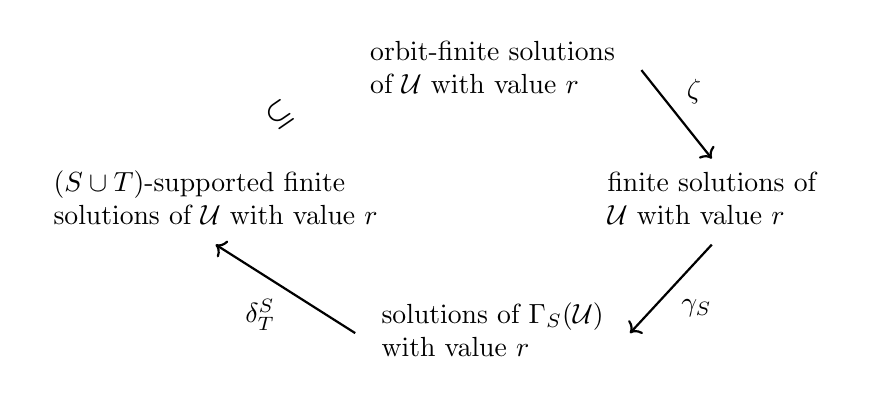
\begin{tikzpicture}
\node (cent) {} ;
\node (ofsol) [above= of cent]
{\begin{tabular}{l}
 orbit-finite solutions\\ of $\cU$ with value $r$
 \end{tabular}};
\node (finsol) [right= of cent]
{\begin{tabular}{l}
 finite solutions of \\ $\cU$ with value $r$
 \end{tabular}};
\node (solfin) [below= of cent]
{\begin{tabular}{l}
 solutions of $\orbSum{S}(\cU)$\\
 with value $r$
 \end{tabular}};
\node (suppsol) [left=of cent]
{\begin{tabular}{l}
 $(S\cup T)$-supported finite \\
 solutions of $\cU$ with value $r$
 \end{tabular}};
\draw[thick,->] (ofsol.east) -- (finsol.north) node[midway,above right] {$\orbres$};
\draw[thick,->] (finsol.south) -- (solfin.east) node[midway,below right] {$\orbsum{S}$};
\draw[thick,->] (solfin.west) -- (suppsol.south) node[midway,below left] {$\orbdis{S}{T}$};
\draw[draw=none] (suppsol.north) -- (ofsol.west) node[midway,sloped] {$\boldsymbol{\subseteq}$};
\end{tikzpicture}
\]
%
%\[
%\xymatrix{
%& \text{orbit-finite solutions of $\cU$} & \\
%& &\text{finite solutions of $\cU$} \\
%\text{finite solutions of $\cU$} & &
%}
%\]
%\[
%\xymatrix{
%\text{orbit-finite solutions of $\cU$}
%\ar@{|->}[r]^{\orbsum{S}}
%& \text{finite solutions of $\cU$}
%\ar@{|->}[d]^{\orbsum{S}}
%& \cU \ar@{|->}[d]^{\orbsum{S}} \\
%& \text{solution of $\orbSum{S}(\cU)$} & \orbsum{S}(\cU)
%}
%\]
%
The dual of the column-finite linear program $\cU$ is the row-finite linear program
%
\begin{equation}\label{eq:row fin dual}
\dualAbc
\end{equation}
%
%Since $\cU$ is an arbitrary column-finite maximisation problem,
%$\transpose{\cU}$ is an arbitrary row-finite minimisation problem.
Call this linear program $\transpose{\cU}$.
The dual of the finite linear program $\orbSum{S}(\cU)$ is
\begin{equation}\label{eq:finite dual}
\lpMin{$\transpose{\orbsum{S}(\vr{b})}\cdot \vr{y}$}{
  $\transpose{\orbSum{S}(\vr{A})}\cdot \vr{y}\leqslant
  \transpose{\orbsum{S}(\transpose{\vr{c}})}$ \\
& $\vr{y}\geqslant \vr{0}$
}
\end{equation}
%
Call this linear program $\transpose{\orbSum{S}(\cU)}$.
%
\begin{definition}\label{def:orbrow}
For an $S$-supported orbit-finite set $S$,
define the \emphdef{orbit distribution function}
\[
\orbrow{S} : \R^{\orbits[S]{D}}\to\lin{D}
\]
as
\[
\orbrow{S}(\vr{x}) : c \mapsto \vr{x}(\orbit[S]{c})\ . 
\]
\end{definition}
%
\begin{lemma}\label{lem:orbrow sol}
If $\vr{y}$ is a solution of $\transpose{\orbSum{S}(\cU)}$ then,
$\orbrow{S}(\vr{y})$ is a solution of $\transpose{\cU}$ and
\[
\transpose{\vr{b}}\cdot\orbrow{S}(\vr{y}) =
\transpose{\orbsum{S}(\vr{b})}\cdot\vr{y}
\]
\end{lemma}
%
\begin{definition}\label{def:orbsmt}
For an $S$-supported orbit-finite set of atom-dimension at least $d$,
define the \emph{semi-orbit summation function}
\[
\orbsmt{S}{T} : (B\to\R)\to(\R^{\orbits[S]{B}})
\]
as
\[
\orbsmt{S}{T}(\vr{v}) :
(K\in\orbits[S]{B})\mapsto
\left(\frac{1}{|K_{S\cup T}|} \cdot \sum_{b\in K_{S\cup T}} \vr{v}(b) \right)
\]
where for $K\in\orbits[S]{B}$ 
\[
K_{S\cup T} = \setof{b\in X}{\text{$b$ is supported by $(S\cup T)$}} \ .
\]
\end{definition}
%
\begin{lemma}\label{lem:orbsmt sol}
If $\vr{y}$ is a solution of $\transpose{\cU}$ then,
$\orbsmt{S}{T}(\vr{y})$ is a solution of $\transpose{\orbSum{S}(\cU)}$ with
\[
\transpose{\vr{b}}\cdot \vr{y} =
\transpose{\orbsum{S}(\vr{b})}\cdot\orbsmt{S}{T}(\vr{y})
\]
\end{lemma}
%
As an immediate corollary of Lemmas \ref{lem:orbrow sol} and \ref{lem:orbsmt sol} we get:
\begin{corollary}\label{cor:row fin solv}
%
The linear programs $\transpose{\cU}$ and $\transpose{\orbSum{S}(\cU)}$ are equivalent.
\end{corollary}
%
\begin{proof}[Proof of Theorem \ref{thm:row fin opt}]
The optimum of $\transpose{\cU}$ can only decrease if we allow the solutions to be orbit-infinite and can only increase if we restrict the solutions to be supported by $S$.
Lemmas \ref{lem:orbrow sol} and \ref{lem:orbsmt sol} together imply that for any solution $\vr{y}$ of $\transpose{\cU}$ (be it orbit-infinite or orbit-finite),
$(\orbrow{S}\circ\orbsmt{S}{T})(\vr{y})$ is an $S$-supported solution of $\transpose{\cU}$ with
\[
\transpose{\vr{b}}\cdot(\orbrow{S}\circ\orbsmt{S}{T})(\vr{y})
= \transpose{\vr{c}}\cdot\vr{y}
\]
Hence the optimum of $\transpose{\cU}$ does not change if either we allow the solutions to be orbit-infinite or we restrict the solutions to be $S$-supported.

Now assume the optimum of $\transpose{\cU}$ is finite (say $r\in\R$).
Corollary \ref{cor:row fin solv} implies the optimum of $\transpose{\orbSum{S}(\cU)}$ is also $r$.
Finite linear programs admit optimal solutions when their optimums are finite.
Let $\vr{z}$ be an optimal solution of $\orbSum{S}(\cU)$.
Then $\orbrow{S}(\vr{z})$ is an $S$-supported finite solution of $\transpose{\cU}$ with
\[
\transpose{\vr{b}}\cdot\orbrow{S}(\vr{z}) = r
\]
Since $r$ is the optimum of $\transpose{\cU}$, $\orbrow{S}(\vr{z})$ is also an optimal solution.
%
%Due to the arbitrariness of the choice $S\subseteqfin\A$, row-finite linear program $\transpose{\cU}$,
%this proves Theorem \ref{thm:row fin opt} for row-finite minimisation problems.
\end{proof}
%
Lemmas \ref{lem:orbrow sol} and \ref{lem:orbsmt sol}, and the proof of Theorem \ref{thm:row fin opt} using them can be summarised by the following diagram.
In this diagram, $r$ represents an arbitrary real number.
\[
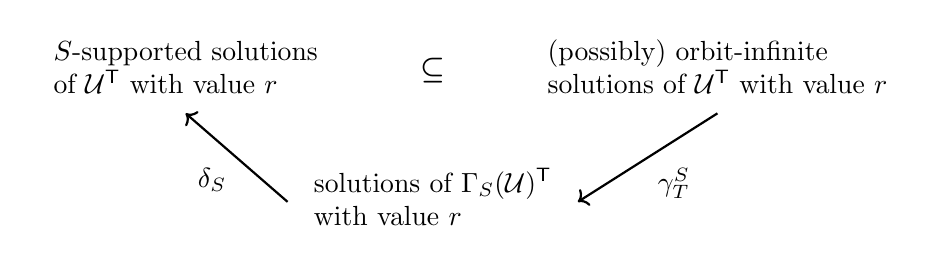
\begin{tikzpicture}
\node (cent) {} ;
\node (infsol) [right=of cent]
{\begin{tabular}{l}
 (possibly) orbit-infinite\\
 solutions of $\transpose{\cU}$ with value $r$
 \end{tabular}};
\node (solfin) [below=of cent]
{\begin{tabular}{l}
 solutions of $\transpose{\orbSum{S}(\cU)}$\\ with value $r$
 \end{tabular}};
\node (suppsol) [left=of cent]
{\begin{tabular}{l}
 $S$-supported solutions \\
 of $\transpose{\cU}$ with value $r$
 \end{tabular}};
\draw[thick,->] (infsol.south) -- (solfin.east) node[midway,below right] {$\orbsmt{S}{T}$};
\draw[thick,->] (solfin.west) -- (suppsol.south) node[midway,below left] {$\orbrow{S}$};
\draw[draw=none] (suppsol.east) -- (infsol.west) node[midway] {$\boldsymbol{\subseteq}$};
\end{tikzpicture}
\]
%
\begin{proof}[Proof of Theorem \ref{thm:col row duality}]
%
%We show that if either the primal or dual is column-finite and
%if the optimum of either of them is finite then, they have the same optimum.
%We do the proof for the case when the primal is column-finite.
%The proof for the other case is similar.
Consider the primal-dual pair $\cU$ -- $\transpose{\cU}$.
Corollary \ref{cor:col fin solv} says that $\cU$ and $\orbSum{S}(\cU)$ have the same optimum.
Similarly, Corollary \ref{cor:row fin solv} says that $\transpose{\cU}$ and $\transpose{\orbSum{S}(\cU)}$ have the same optimum.
The pair $\orbSum{S}(\cU)$ -- $\transpose{\orbSum{S}(\cU)}$ is a primal-dual pair of finite linear programs.
Hence if the optimum of any of the linear programs $\cU$ or $\transpose{\cU}$ is finite then using the classical duality theorem we can conclude that the it is equal to the optimum of the other.
%Since the pair $\cU$-$\transpose{\cU}$ is an arbitrary primal-dual pair of orbit-finite linear program where the primal is column-finite, this finishes the proof of the theorem for the case when the primal is column-finite.
%The proof of the other case is similar and so we skip it.
\end{proof}
%
\begin{remark}
\arka{$L_1$-norm bounded solutions of column-finite systems.
Maybe update the theorem}
\end{remark}
%
\begin{example}
Let $S = \emptyset$.
Let $\star$ be an equivariant element,
i.e.\ $\pi(\star)=\star$ for every $\pi\in\aut{\A}$.
Let $B = \{\star\}\uplus\A$ and $C = \A^2$.
The set $B$ has two equivariant orbits,
namely $\{\star\}$ and $\A$,
and $C$ also has two equivariant orbits,
namely $\A^{(2)} = \setof{\a\b\in C}{\a\neq\b}$
and $I = \setof{\a\a}{\a\in\A}$.
For every $(\a,\b)\in C$ define $\vr{v}_{\a\b}\in\flin{B}$ as
\[
\vr{v}_{\a\b}\defeq
\begin{cases}
\a + \b + \star & \text{if }\a\neq\b \\
\star - \a& \text{otherwise.}
\end{cases}
\]
For every $(\a,\b)\in C$
we have $\orbsum{S}(\vr{v}_{\a\b})\in\R^{\orbits[S]{B}} = \R^2$ and
\[
\orbsum{S}(\vr{v}_{\a\b}) =
\begin{cases}
(2,1) & \text{if }\a\neq\b \\
(1,-1) & \text{otherwise.}
\end{cases}
\]
(assuming that the first and the second coordinate, respectively,
correspond to the orbits $\A$ and $\{\star\}$).
Define $\vr{A}$ to be the $(B{\times} C)$ matrix with columns $\vr{A}(-,\a\b) = \vr{v}_{\a\b}$ for $c\in C$.
Then $\vr{A}$ is a column-finite matrix.
We have
\[
\begin{tabular}{l l}

& \indexcolor{\phantom{...} $\otuequiv{2}$ $\phantom{.....}$ $I$} \\

$\orbSum{S}(\vr{A})\ \ =$

& $
\begin{bmatrix}
\phantom{a}2\phantom{a} & \phantom{a}-1\phantom{a} \\
\phantom{a}1\phantom{a} & \phantom{a.....}1\phantom{a} \\
\end{bmatrix}
$

\indexcolor{
$
\begin{tabular}{c}
$\A$ \\
$\set{\star}$
\end{tabular}
$
}

\end{tabular}
\]
Define $\vr{b}\in\flin{B}$ and $\vr{c}\in\lin{C}$ as
\[
\vr{b} = \star \quad\text{and}\quad \vr{c} = 2\cdot\idvec{\otuequiv{2}} +\idvec{I}
\ .
\]
Using $\vr{A}$, $\vr{b}$ and $\vr{c}$ we form $\cU$ to be the column-finite linear program
%
\begin{equation}\label{eq:primal eg}
\lpMatPrimal{\vr{A}}{\vr{b}}{\vr{c}}{\vr{x}}{B}{C}
\end{equation}
%
The vector $\vr{b}$ is an equivariant finite vector.
Hence $\orbSum{S}(\vr{b}) = \orbsum{S}(\vr{b}) = (0,1)$.
Since $\vr{c}$ is not a finite vector $\orbsum{S}(\vr{c})$ is not well-defined.
However, following usual convention we consider
$\transpose{\vr{c}}$ to be a row vector (i.e.\ matrix with only one row),
and hence it is automatically column-finite.
Moreover $\transpose{\vr{c}}$ is equivariant.
Hence $\orbSum{S}(\transpose{\vr{c}})$ is well-defined and is equal to
\[
\begin{tabular}{l l}
& \indexcolor{\phantom{..}$\otuequiv{2}$ \quad $I$} \\

$\orbSum{S}(\transpose{\vr{c}})\ \ =$

& $
\begin{bmatrix}
\phantom{.}2\phantom{...} & \phantom{...}1\phantom{.}
\end{bmatrix}
\ .
$
\end{tabular}
\]
%
Using $\orbSum{S}$ we get the finite linear program
\[
\orbSum{S}(\cU) :
\lpMax{$2\cdot x_1 + x_2$}
{   $         2\cdot x_1 - x_2 \leqslant 0$ \\
  & $\phantom{.....}x_1 + x_2 \leqslant 1$}
\]
%
%\begin{equation}\label{eq:finite primal eg}
%\lpMax{$\orbSum{S}(\transpose{\vr{c}})\cdot \vr{x}$}{
%  $\orbSum{S}(\vr{A}) \cdot \vr{x} \leqslant \orbSum{S}(\vr{b})$ \\
%& $\vr{x} \geqslant \vr{0}$
%}
%\end{equation}
%%
%Call this $\orbSum{S}(\cU)$.
%
Fix some $\a_1\b_1\tau_1\in\otuequiv{3}$.
Define $\vr{x}\in\flin{B}$ as
\[
\vr{x} = \frac{1}{9}\cdot\left(2\cdot\a_1\b_1 + \b_1\tau_1
 + 2\cdot\a_1\a_1 + 3\cdot\b_1\b_1 + \tau_1\tau_1 \right)\ .
\]
Then $\vr{x}$ is a non-negative finite solution with value $\frac{4}{3}$, since
\[
\vr{A}\cdot\vr{x} = \star = \vr{b},
\quad\text{and}\quad
\transpose{\vr{c}}\cdot\vr{x} = \frac{4}{3} \ .
\]
We have $\orbsum{S}(\vr{x}) = \left(\frac{1}{3},\frac{2}{3}\right)$.
Since
\[
\orbSum{S}(\vr{A})\cdot\orbsum{S}(\vr{x}) = \left(1,0\right) = \orbSum{S}(\vr{b}),
\quad\text{and}\quad
\orbsum{S}(\transpose{\vr{c}})\cdot\orbsum{S}(\vr{x}) = \frac{4}{3}
\]
the vector $\orbsum{S}(\vr{x})$ is a non-negative solution of $\orbSum{S}(\cU)$ with value $\frac{4}{3}$.
Coincidentally it is also an optimal solution,
and in this case the unique one.
The atom dimension of $\cU$ is $2$.
Let $T = \set{\a_1,\b_1}$.
Then
\[
\orbdis{S}{T}(\orbsum{S}(\vr{x})) =
\frac{1}{6}\cdot\left(\a_1\b_1 + \b_1\a_1\right) + 
\frac{1}{3}\cdot\left(\a_1\a_1 + \b_1\b_1\right)
\]
The vector $\orbdis{S}{T}(\orbsum{S}(\vr{x}))$ is non-negative.
Furthermore, $\vr{A}\cdot\orbdis{S}{T}(\orbsum{S}(\vr{x})) = \star = \vr{b}$, and ${\transpose{\vr{c}}\cdot\orbdis{S}{T}(\orbsum{S}(\vr{x})) = \frac{4}{3}}$.
Hence $\orbdis{S}{T}(\orbsum{S}(\vr{x}))$ is a solution of $\cU$ and in this case an optimal one.
\arka{say we got a smaller solution}

%The dual of the column-finite linear program \eqref{eq:primal eg} is the row-finite linear program
%\begin{equation}\label{eq:dual eg}
%\lpMinPrimal{\transpose{(\vr{A})}}{\vr{c}'}{(\vr{b})}{\vr{y}}{C}{B}
%\end{equation}
%And the dual of the finite linear program \eqref{eq:finite primal eg} is the linear program
%\begin{equation}\label{eq:finite dual eg}
%%\lpMinPrimal{\transpose{\orbSum{S}(\vr{A})}}{\orbSum{S}(\vr{b})}{\orbSum{S}\vr{c}}{\vr{y}}{C}{B}
%\lpMin{$\transpose{\orbSum{S}(\vr{b}')}\cdot \vr{y}$}{
%  $\transpose{\orbSum{S}(\vr{A})}\cdot \vr{y} \geqslant \transpose{\orbSum{S}(\transpose{\vr{c}})}$ \\
%  & $\vr{y} \geqslant \vr{0}$
%} 
%\end{equation}

Pick an infinite subset $W\subseteq\A$.
Define $\vr{y}_W = 3\cdot\star + \idvec{W} + 2\cdot\idvec{(\A\setminus W)}$.
The vector $\vr{y}_W$ is an orbit-infinite solution of $\transpose{\cU}$ with value $3$. 
The result $\orbsmt{S}{T}(\vr{y}_W)$ of applying $\orbsmt{S}{T}$ to $\vr{y}_W$ depends on the intersection $\set{\a,\b}\cap W$.
We focus on the case where $\set{\a,\b}\cap W = \set{\a}$,
the remaining cases can be dealt with similarly.
In this case, $\orbsmt{S}{T}(\vr{y}_W) = (\frac{3}{2},3)$ (assuming that the first and the second co-ordinate, respectively,
corresponds to the orbits $\A$ and $\set{\star}$).
Dualising $\orbSum{S}(\cU)$ we get
\[
\transpose{\orbSum{S}(\cU)} :
\lpMin{$y_2$}
{   $2\cdot y_1 + y_2 \geqslant 2$ \\
  & $\ \, -y_1 + y_2 \geqslant 1$}
\]
The vector $\orbsmt{S}{T}(\vr{y}_W)$ is a solution with of $\transpose{\orbSum{S}(\cU)}$ with value $3$.
Applying $\orbrow{S}$ to $\orbsmt{S}{T}(\vr{y}_W)$ we get
\[
\orbrow{S}(\orbsmt{S}{T}(\vr{y}_W)) = 3\cdot\star + \frac{3}{2}\cdot\idvec{A}
\] 
which is an equivariant solution of $\transpose{\cU}$ with value $3$.
\arka{say we got an equivariant solution}
\end{example}
%
\section{The orbit summation function}\label{sec:orbsum}
%
\begin{lemma}\label{lem:cod orbsum S supp}
Every element in $\R^{\orbits[S]{D}}$ is supported by $S$.
\end{lemma}
%
\begin{proof}
Pick arbitrary $\vr{v}\in\R^{\orbits[S]{D}}$, $\pi\in\aut[S]{\A}$ and $K\in\orbit[S]{D}$.
We have $\pi^{-1}(K) = K$.
Using this and \Cref{lem:perm fun}
\[
\pi(\vr{v})(K) = \vr{v}(\pi^{-1}(K)) = \vr{v}(K) \ .
\]
\end{proof}
%
\begin{lemma}\label{lem:orbsum prop}
The function $\orbsum{S}$ % : \flin{D} \to \R^{\orbits[S]{D}}$
is an $S$-supported monotonic linear map.
\end{lemma}
%
\begin{proof}
Linearity and monotonicity of $\orbsum{S}$ follows easily from its definition.
We focus on proving that it is supported by $S$.

Pick arbitrary $\vr{v}\in\flin{D}$ and $\pi\in\aut[S]{\A}$.
Using item \textit{(ii)} we get that
$\pi(\orbsum{S}(\vr{v})) = \orbsum{S}(\vr{v})$.
Also for any $K\in\orbits[S]{D}$ using Lemma \ref{lem:perm orb aut} we get
\begin{align*}
\orbsum{S}(\pi(\vr{v}))(K) & =
\sum_{b\in K} \pi(\vr{v})(b) &  \\
& = \sum_{b\in K} \vr{v}(\pi^{-1}(b)) &  \\
& = \sum_{b\in K} \vr{v}(\pi^{-1}(b)) = \orbsum{S}(\vr{v})(K)
\end{align*}
Hence $\orbsum{S}(\pi(\vr{v}))(K) = \orbsum{S}(\vr{v}) = \pi(\orbsum{S}(\vr{v}))$,
which finishes the proof.
\end{proof}
%
\begin{lemma}\label{lem:orbsum matrix well def}
The function $\orbSum{S}$ is well-defined for $S$-supported column-finite matrices.
%For any $L\in\orbits[S]{E}$ and $c,c'\in L$
%\[
%\orbsum{S}(\vr{B}(-,c)) = \orbsum{S}(\vr{B}(-,c'))
%\]
%
\end{lemma}
%
\begin{proof}
%
Since $c$ and $c'$ are in the same $S$-orbit,
there exists $\pi\in\aut[S]{\A}$ such that $\pi(c)=c'$.
We have the following sequence of equalities which completes the proof.
\begin{align*}
&& \orbsum{S}(\vr{B}(-,c))\quad=\quad
& \pi(\orbsum{S}(\vr{B}(-,c)))
& \text{(\Cref{lem:cod orbsum S supp})}\\
&&=\quad
& \orbsum{S}(\pi(\vr{B}(-,c)))
& \text{(\Cref{lem:orbsum prop})}\\
&&=\quad
& \orbsum{S}(\vr{B}(-,\pi(c)))
& \text{(\Cref{lem:perm im S supp})} \\
&&=\quad
& \orbsum{S}(\vr{B}(-,c')\ .
\end{align*}
\end{proof}
%
%As we promised,
%now we show that this definition indeed achieves what we intended it to.
%%
%\arka{actually this lemma is superfluous now}
%
%\begin{lemma}\label{lem:orbsum matrix}
%For a column-finite $B{\times} C$-matrix $\vr{A}$ supported by $S$
%\[
%\orbsum{S}({\setof{\vr{A}(-,c)}{c\in C}}) =
%\setof{(\orbSum{S}(\vr{A}))(-,L)}{L\in \orbits[S]{C}}
%\]
%\end{lemma}
%%
%\begin{proof}
%\[
%\begin{aligned}
%  & \orbsum{S}({\setof{\vr{A}(-,c)}{c\in C}}) \\
%= & \setof{\orbsum{S}(\vr{A}(-,c))}{c\in C} \\
%= & \setof{(\orbSum{S}(\vr{A}))(-,\orbit[S]{c})}{c\in C} \\
%= & \setof{(\orbSum{S}(\vr{A}))(-,L)}{L\in \orbits[S]{C}}
%\end{aligned}
%\]
%\end{proof}
%
\begin{lemma}\label{lem:orbsum mat vec}
For any $S$-supported column-finite matrix $\vr{B}\in\lin{D{\times}C}$ and vector $\vr{x}\in\flin{C}$ we have
$\orbsum{S}(\vr{B}\cdot\vr{x}) = \orbSum{S}(\vr{B})\cdot\orbsum{S}(\vr{x})$.
\end{lemma}
%
\begin{proof}
Pick arbitrary $K\in\orbits[S]{D}$.
We show
\[
\orbsum{S}(\vr{B}\cdot\vr{x})(K) = (\orbSum{S}(\vr{B})\cdot\orbsum{S}(\vr{x}))(K)
\ .
\]
The following sequence of equations finish the proof
\begin{align*}
&& \orbsum{S}(\vr{B}\cdot\vr{x})(K) =
&  \sum_{b\in K} (\vr{B}\cdot\vr{x})(b)
& \text{(Definition \ref{def:orbsum vector})} \\
&& =
& \sum_{b\in K}\sum_{c\in C}\vr{A}(b,c)
& \\
&& =
& \sum_{b\in K}\sum_{M\in\orbits[S]{C}}\sum_{c\in M}\vr{B}(b,c)\cdot\vr{x}(c)
& \\
&& =
&\sum_{M\in\orbits[S]{C}}
 \sum_{c\in M}\vr{x}(c)\cdot\left(
 \sum_{b\in K}\vr{B}(b,c)\right)
& \text{(rearrangement)} \\
&& =
& \sum_{M\in\orbits[S]{C}}
  \sum_{c\in M}\vr{x}(c)\cdot\orbSum{S}(\vr{A})(K,M)
& \text{(Definition \ref{def:orbsum matrix})}\\
&& =
& \sum_{M\in\orbits[S]{C}}\orbSum{S}(\vr{B})(K,M)\cdot
  \sum_{c\in M}\vr{x}(c)
& \text{(rearrangement)} \\
&& =
& \sum_{M\in\orbits[S]{C}}\orbSum{S}(\vr{B})(K,M)\cdot\orbsum{S}(\vr{x})(M)
& \text{(Definition \ref{def:orbsum vector})}\\
&& =
& \ (\orbSum{S}(\vr{A})\cdot\orbsum{S}(\vr{x}))(K)\ . \\
\end{align*}
\end{proof}
%
\begin{corollary}\label{cor:orbsum mat prod}
The function $\orbSum{S}$ commutes with matrix multiplication.
%For $S$-supported column-finite matrices $\vr{B}\in\lin{D{\times}E}$ and $\vr{C}\in\lin{E{\times}F}$ we have
%$\orbSum{S}(\vr{B}\cdot\vr{C}) = \orbSum{S}(\vr{B})\cdot\orbSum{S}(\vr{C})$.
\end{corollary}
%
\begin{proof}
Let $L$ be an arbitrary element of $\orbits[S]{F}$.
We show
\[
\orbsum{S}(\vr{B}\cdot\vr{C})(-,L) =
(\orbSum{S}(\vr{B})\cdot\orbSum{S}(\vr{C}))(-,L)
\]
Let $d$ be an arbitrary element of $F$.
\begin{align*}
   & (\orbSum{S}(\vr{B}\cdot\vr{C}))(-,L)
   & \\
=\ & \orbSum{S}((\vr{B}\cdot\vr{C})(-,d))
   & \text{(Definition \ref{def:orbsum matrix})} \\
=\ & \orbSum{S}(\vr{B}\cdot\vr{C}(-,d))
   & \\
=\ & \orbSum{S}(\vr{B})\cdot\orbSum{S}(\vr{C}(-,d))
   & \text{(Lemma \ref{lem:orbsum mat vec})} \\
=\ & \orbSum{S}(\vr{B})\cdot(\orbSum{S}(\vr{C}))(-,L)
   & \text{(Definition \ref{def:orbsum matrix})} \\
=\ & (\orbSum{S}(\vr{B})\cdot\orbSum{S}(\vr{C}))(-,L) \ .
   &  \\
\end{align*}
\end{proof}
%
\begin{corollary}\label{cor:orbsum prod}
For any $\vr{x}\in\flin{C}$ we have
$\orbSum{S}(\transpose{\vr{c}})\cdot\orbsum{S}(\vr{x})
=\transpose{\vr{c}}\cdot\vr{x}$.
\end{corollary}
%
\begin{proof}
Assuming $E = C$ and $D$ to be a singleton, from \Cref{lem:orbsum mat vec} we get
$\orbSum{S}(\transpose{\vr{c}})\cdot\orbsum{S}(\vr{x})=
\orbsum{S}(\transpose{\vr{c}}\cdot\vr{x})$.
But $\transpose{\vr{c}}\cdot\vr{x}$ is a just a number,
so it is safe to write
$\orbsum{S}(\transpose{\vr{c}}\cdot\vr{x}) = \transpose{\vr{c}}\cdot\vr{x}$.
\end{proof}
%
\begin{lemma}\label{lem:orbsum ptime}
The function $\orbSum{S}$ is computable in \exptime{} and in \ptime{} in fixed atom-dimension.
\end{lemma}
%
\arka{TODO: cite representation given in \Cref{ch:equations}}
%
\begin{proof}[Proof of Lemma \ref{lem:orbsum ptime}]
The dimension of $\orbSum{S}(\vr{A})$ is $\orbits[S]{B}{\times}\orbits[S]{C}$,\\
which is polynomial in the size of the standard representation of $\vr{A}$.
Hence, it is enough to show that every entry of $\orbSum{S}(\vr{A})$ can be computed in \fadp.
Pick arbitrary $(K,L)\in\orbits[S]{B}{\times}\orbits[S]{C}$.
Say $b$ and $c$ are respectively the representative elements of $X$ and $Y$ in the standard representation of $\vr{A}$.
We want to compute
\[
\orbSum{S}(\vr{A})(K,L) = \sum_{b'\in K} \vr{A}(b',c) \ .
\]
Let $K'\subseteq K$ be the set of elements in $K$ which are supported by ${(S\cup\supp{c})}$.
Lemma \ref{lem:col fin supp} implies
\[
\setof{b'\in K}{\vr{A}(b',c)\neq 0}\subseteq K' \ .
\]
Hence it is enough to compute $\sum_{b'\in K'} \vr{A}(b',c)$.
We have two cases:
%
\paragraph{(Case 1: $|\supp{b}\setminus S| > |\supp{c}\setminus S|$)}
%
In this case, Lemma \ref{lem:pick elem supp} implies $K'$ is empty.
Hence $\sum_{b'\in K'} \vr{A}(b',c) = 0$.
%
\paragraph{(Case 2: $|\supp{b}\setminus S| \leqslant |\supp{c}\setminus S|$)}
%
In this case, we can compute some $b'\in K'$ using Lemma \ref{lem:pick elem supp}.
By Lemma \ref{lem:supp aut T} we get
\[
K' = \aut{\supp{c}\setminus S}\cdot\set{b'} \ .
\]
Let $d$ be the atom-dimension of $\vr{A}$.
Then $|\aut{\supp{c}\setminus S}|\leqslant d!$.
Hence, using Lemmas \ref{lem:apply perm fadp} and \ref{lem:eq check fadp} we can compute $K'$ in \fadp{}. 
For every $b'\in K'$ we can compute $\vr{A}(b',c)$ in \fadp{} (Lemma \ref{lem:matrix query ptime}).
\arka{remove \fadp{}}
Hence we can also compute $\sum_{b'\in K'} \vr{A}(b',c)$ in \fadp{}.
%
\end{proof}
%
\begin{proof}[Proof of Lemma \ref{lem:orbsum sol}]
Consider an arbitrary solution $\vr{x}$ of $\cU$.
Then $\vr{A}\cdot\vr{x} \leqslant{\vr{b}}$.
By \Cref{lem:orbsum prop}, $\orbsum{S}(\vr{x})$ is non-negative.
Applying \Cref{lem:orbsum mat vec} we get
%
\begin{equation}\label{eq:orbsum sol 1}
\orbSum{S}(\vr{A})\cdot\orbsum{S}(\vr{x}) =
\orbsum{S}(\vr{A}\cdot\vr{x}) \ .
\end{equation}
%
From $\vr{A}\cdot\vr{x}\leqslant\vr{b}$,
using Lemma \Cref{lem:orbsum prop} we get
%
\begin{equation}\label{eq:orbsum sol 2}
\orbsum{S}(\vr{A}\cdot\vr{x}) \leqslant \orbSum{S}(\vr{b}) \ .
\end{equation}
Combining equation \eqref{eq:orbsum sol 1} with inequality \eqref{eq:orbsum sol 2} we get
\[
\orbSum{S}(\vr{A})\cdot\orbsum{S}(\vr{x}) \leqslant
\orbSum{S}(\vr{b}) \ .
\]
Hence, $\orbsum{S}(\vr{x})$ is a solution of $\orbSum{S}(\cU)$.
Finally \Cref{cor:orbsum prod} gives us
\[
\orbsum{S}(\transpose{\vr{c}})\cdot\orbsum{S}(\vr{x}) =
\transpose{\vr{c}}\cdot\vr{x} \ .
\]
\end{proof}
%
\section{The semi-orbit distribution function}\label{sec:orbdis}
%
Immediately from the definition of $\orbdis{S}{T}$ we get:
%
\begin{lemma}\label{lem:orbdis lin}
The function $\orbdis{S}{T}$ %: \R^{\orbits[S]{D}}\to\flin{D}$
is a monotonic linear map.
\end{lemma}
%
\begin{definition}\label{def:supp S T}
A set $x$ is said to be supported by $(S\cup\{T\})$ if it is supported by $(S\cup T)$ and is invariant under $\aut{T}$, i.e.
\[
\pi(x) = x
\ \ \text{for all}\ \
\pi\in\aut{T}\ .
\]
\end{definition}
%
\begin{lemma}\label{lem:supp S implies S T}
If a set $x$ is supported by $S$ then it is also supported by $(S\cup\set{T})$.
\end{lemma}
%
\begin{proof}
Follows from the fact that
$\aut[S\cup T]{\A}\cup\aut{T}\subseteq \aut[S]{\A}$.
\end{proof}
%
\begin{lemma}\label{lem:orbdis supp}
For any $\vr{x}\in\R^{\orbits[S]{D}}$ the vector $\orbdis{S}{T}(\vr{x})$ is finite and is supported by ${(S\cup\set{T})}$.
\end{lemma}
%
\begin{proof}
Consider an arbitrary $\vr{x}\in\R^{\orbits[S]{B}}$.
We need to show that $\orbdis{S}{T}(\vr{x})$ is supported by $(S\cup\set{T})$.
First we show $\orbdis{S}{T}(\vr{x})$ is supported by $(S\cup T)$.
The vector $(\orbdis{S}{T}(\vr{x}))(b)\neq 0$ only if $b\in X'$ for some $X\in\orbits[S]{B}$.
Lemma \ref{lem:supp aut T} implies that for every $X\in\orbits[S]{B}$,
the set $X'$ is finite.
Hence  $\orbdis{S}{T}(\vr{x})$ is also a finite vector.
By definition, every element of $X'$ is supported by $(S\cup T)$.
Applying Lemma \ref{lem:fin vec supp} we conclude $\orbdis{S}{T}(\vr{x})$ is supported by \\ $(S\cup T)$.

Now we show that for any $\pi\in\aut{T}$ we have
$(\pi\circ\orbdis{S}{T})(\vr{x}) = \vr{x}$.
Pick arbitrary $\pi\in\aut{T}$.
Applying Lemma \ref{lem:add equiv} we get
\begin{equation}\label{eq:orbdis supp 4}
(\pi\circ\orbdis{S}{T})(\vr{x}) =
\left(
\sum_{X\in\orbits[S]{B}}
\frac{\vr{x}(X)}{|X'|} \cdot \sum_{b\in X'} \pi(b)
\right)
\end{equation}
Lemma \ref{lem:supp aut T} implies the set $\pi(X') = X'$.
Then $\pi$ induces a permutation of $X'$ (with $\pi^{-1}$ inducing the inverse permutation).
Hence
\begin{equation}\label{eq:orbdis supp 5}
\sum_{b\in X'} \pi(b) = \sum_{b\in X'} b
\end{equation}
Using equations \eqref{eq:orbdis supp 4} and \eqref{eq:orbdis supp 5} we conclude
\[
(\pi\circ\orbdis{S}{T})(\vr{x})
=
\left(
\sum_{X\in\orbits[S]{B}}
\frac{\vr{x}(X)}{|X'|} \cdot \sum_{b\in X'} b
\right)
= \orbdis{S}{T}(\vr{x})
\]
Since $\pi\in\aut{T}$ was arbitrarily chosen,
this proves for any $\pi\in\aut{T}$ we have
$(\pi\circ\orbdis{S}{T})(\vr{x}) = \vr{x}$.
Since $\vr{x}\in\R^{\orbits[S]{B}}$ was arbitrarily chosen,
this finishes the proof of the lemma.
\end{proof}
%
\begin{lemma}\label{lem:orbsum orbdis inv}
$\orbsum{S}\circ\orbdis{S}{T} = \id$.
\end{lemma}
%
\begin{proof}
\arka{Remove the proof if it is obvious}

\noindent
Pick arbitrary $\vr{x}\in\R^{\orbits[S]{B}}$.
Using the definition of $\orbdis{S}{T}(\vr{x})$
\begin{equation}\label{eq:orbsum orbsum inv 1}
\orbdis{S}{T}(\vr{x}) =
\sum_{K\in\orbits[S]{B}}\left(
\frac{\vr{x}(K)}{|K_{S\cup T}|} \cdot \sum_{b\in K_{S\cup T}} b
\right)\ ,
\end{equation}
where for $K\in\orbits[S]{B}$ the set
\[
K_{S\cup T} = \setof{b\in K}{\supp{b}\subseteq (S\cup T)} \ .
\]
Pick arbitrary $K\in\orbits[S]{B}$.
For $b\in B$ we have $((\orbdis{S}{T}(\vr{x}))(b))(K) = 1$ if $b\in K$,
otherwise $((\orbdis{S}{T}(\vr{x}))(b))(K) = 0$.
Now applying linearity of $\orbsum{S}$ (Lemma \ref{lem:orbsum lin S supp}) to equation \eqref{eq:orbsum orbsum inv 1} we get
\[
(\orbsum{S}(\orbdis{S}{T}(\vr{x})))(K) = 
\frac{\vr{x}(K)}{|K_{S\cup T}|} \cdot |K_{S\cup T}| = \vr{x}(K)
\]
Since $K\in\orbits[S]{B}$ was chosen arbitrarily this proves
\[
\orbsum{S}(\orbdis{S}{T}(\vr{x})) = \vr{x}
\]
Since $\vr{x}\in\R^{\orbits[S]{B}}$ was chosen arbitrarily this finishes the proof of the lemma.
\end{proof}
%
\begin{lemma}\label{lem:orbdis orbsum inv}
For any vector $\vr{x}\in\flin{D}$ supported by ${(S\cup\set{T})}$
\[
(\orbdis{S}{T}\circ\orbsum{S})(\vr{x}) = \vr{x}
\]
\end{lemma}
%
\begin{proof}[Proof of Lemma \ref{lem:orbdis orbsum inv}]
Pick arbitrary $\vr{x}\in\flin{B}$ supported by ${(S\cup\set{T})}$ and $b\in B$.
We show
\[
((\orbdis{S}{T}\circ\orbsum{S})(\vr{x}))(b) = \vr{x}(b)
\]
We split the proof into two cases.

\paragraph{(Case 1: $b$ is not supported by $S\cup T$)}
The vector $\vr{x}$ is a finite vector supported by $(S\cup T)$.
Lemma \ref{lem:orbdis supp} implies $(\orbdis{S}{T}\circ\orbsum{S})(\vr{x})$ is also a finite vector supported by $(S\cup T)$.
Applying Lemma \ref{lem:fin vec supp}
\[
((\orbdis{S}{T}\circ\orbsum{S})(\vr{x}))(b) = 0 = \vr{x}(b)
\]

\paragraph{(Case 2: $b$ is supported by $S\cup T$)}
Let $Y = \orbit[S]{b}$.
Expanding the expression $(\orbdis{S}{T}\circ\orbsum{S})(\vr{x})$ using the definition of $\orbdis{S}{T}$ and $\orbsum{S}$ (Definition \ref{def:orbsum vector})
\[
(\orbdis{S}{T}\circ\orbsum{S})(\vr{x}) =
\sum_{X\in\orbits[S]{B}}
\frac{(\orbsum{S}(\vr{x}))(X)}{|X'|} \cdot
\left(
\sum_{b'\in X'} b'
\right)
\]
By definition of $Y'$ we have $b\in Y'$.
Hence
\[
((\orbdis{S}{T}\circ\orbsum{S})(\vr{x}))(b) =
\frac{(\orbsum{S}(\vr{x}))(Y)}{|Y'|}
\]
To finish the proof we need to show
\[
\vr{x}(b) = \frac{(\orbsum{S}(\vr{x}))(Y)}{|Y'|}
\]
%
\begin{claim}\label{clm:lem:orbdis orbsum inv}
For any $b'\in Y'$ we have $\vr{x}(b) = \vr{x}(b')$.
\end{claim}
%
\begin{claimproof}
Pick arbitrary $b'\in Y'$.
Using Lemma \ref{lem:supp aut T} we can find $\pi\in\aut{T}$ such that $\pi(b) = b'$.
Since $\vr{x}$ is supported by $(S\cup\set{T})$, we have
\[
\pi^{-1}(\vr{x}) = \vr{x}
\]
Using Lemma \ref{lem:perm fun} we get
\[
\vr{x}(b') = \vr{x}(\pi(b)) = (\pi^{-1}(\vr{x}))(b) = \vr{x}(b)
\]
Since $b'\in Y'$ was chosen arbitrarily chosen,
this finishes the proof of the claim.
\end{claimproof}
%
Since $\vr{x}$ is supported by $S\cup T$,
if $\vr{x}(b')\neq 0$ for some $b'\in Y$ then $b'\in Y'$.
This implies
\[
  \sum_{b'\in Y'} \vr{x}(b')
= \sum_{b'\in Y} \vr{x}(b')
= (\orbsum{S}(\vr{x}))(Y)
\]
Now the above claim implies
\[
\vr{x}(b) = \frac{(\orbsum{S}(\vr{x}))(Y)}{|Y'|}
\]
which finishes the proof for this case.

Since $\vr{x}\in\flin{B}$ was chosen to be an arbitrary $S$-supported vector and $b$ was chosen to be an arbitrary element of $B$,
this finishes the proof of the lemma.
\end{proof}
%
\arka{The matrix $\vr{B}$ can not be fixed since then we can not state the corollary in unambiguously}
%
\begin{lemma}\label{lem:orbdis mat vec}
For any $S$-supported column-finite matrix $\vr{B}\in\lin{D{\times}C}$ and vector ${\vr{x}\in\R^{\orbits[S]{C}}}$
\[
\vr{B}\cdot\orbdis{S}{T}(\vr{x}) =
\orbdis{S}{T}(\orbSum{S}(\vr{B})\cdot\vr{x})
\]
\end{lemma}
%
\begin{proof}
Pick arbitrary column-finite matrix $\vr{A}\in\lin{B{\times} C}$ supported by $S$ and arbitrary vector ${\vr{x}\in\R^{\orbits[S]{B}}}$
%
\begin{claim}\label{clm:orbdis mat vec}
$\vr{A}\cdot\orbdis{S}{T}(\vr{x})$ is supported by $(S\cup\set{T})$.
\end{claim}
%
\begin{claimproof}
First we show $\vr{A}\cdot\orbdis{S}{T}(\vr{x})$ is supported by $(S\cup T)$.
The matrix $\vr{A}$ is supported by $S$ and hence also by $(S\cup T)$.
Lemma \ref{lem:orbdis supp} implies that the vector $\orbdis{S}{T}(\vr{x})$ are both supported by $(S\cup T)$.
For any $\pi\in\aut[S\cup T]{\A}$ using Lemma \ref{lem:mult equiv} we get
\[
\pi(\vr{A} \cdot    \orbdis{S}{T}(\vr{x})) =
\pi(\vr{A})\cdot\pi(\orbdis{S}{T}(\vr{x})) =
    \vr{A} \cdot    \orbdis{S}{T}(\vr{x})
\]
Hence $\vr{A}\cdot\orbdis{S}{T}(\vr{x})$ is supported by $(S\cup T)$.

Now we show that for any $\pi\in\aut{T}$
\[
\pi(\vr{A}\cdot\orbdis{S}{T}(\vr{x})) = \vr{A}\cdot\orbdis{S}{T}(\vr{x})
\]
Pick an arbitrary $\pi\in\aut{T}$.
Since $\aut{T}\subseteq\aut[S]{\A}$ and $\vr{A}$ is supported by $S$ we have
$\pi(\vr{A}) = \vr{A}$.
Lemma \ref{lem:orbdis supp} implies
$\pi(\orbdis{S}{T}(\vr{x})) = \orbdis{S}{T}(\vr{x})$.
Applying Lemma \ref{lem:mult equiv} we get
\[
\pi(\vr{A} \cdot    \orbdis{S}{T}(\vr{x})) =
\pi(\vr{A})\cdot\pi(\orbdis{S}{T}(\vr{x})) =
    \vr{A} \cdot    \orbdis{S}{T}(\vr{x})
\]
Since $\pi\in\aut{T}$ was chosen arbitrarily,
this finishes the proof of the claim.
\end{claimproof}
%
Using the above claim and Lemma \ref{lem:orbdis orbsum inv} we get
%
\begin{equation}\label{eq:orbdis mat vec 1}
\vr{A}\cdot\orbdis{S}{T}(\vr{x}) =
(\orbdis{S}{T}\circ\orbsum{S})(\vr{A}\cdot\orbdis{S}{T}(\vr{x}))
\end{equation}
%
Applying Lemma \ref{lem:orbsum mat vec} we get
\begin{equation}\label{eq:orbdis mat vec 2}
(\orbdis{S}{T}\circ\orbsum{S})(\vr{A}\cdot\orbdis{S}{T}(\vr{x})) =
\orbdis{S}{T}(\orbSum{S}(\vr{A})\cdot(\orbsum{S}\circ\orbdis{S}{T})(\vr{x}))
\end{equation}
Lemma \ref{lem:orbsum orbdis inv} implies
$(\orbsum{S}\circ\orbdis{S}{T})(\vr{x}) = \vr{x}$.
Hence
\begin{equation}\label{eq:orbdis mat vec 3}
  \orbdis{S}{T}(\orbSum{S}(\vr{A})\cdot(\orbsum{S}\circ\orbdis{S}{T})(\vr{x}))
= \orbdis{S}{T}(\orbSum{S}(\vr{A})\cdot\vr{x})
\end{equation}
Combining equations
\eqref{eq:orbdis mat vec 1},
\eqref{eq:orbdis mat vec 2} and
\eqref{eq:orbdis mat vec 3}
we get
\[
  \vr{A}\cdot\orbdis{S}{T}(\vr{x})
= \orbdis{S}{T}(\orbSum{S}(\vr{A})\cdot\vr{x})
\]
Since $\vr{x}\in\R^{\orbits[S]{C}}$ is an arbitrary vector,
this finishes the proof of lemma.
\end{proof}
%
Putting $\vr{B} = \transpose{\vr{c}}$ we get:
%
\begin{corollary}\label{cor:orbdis prod}
For any $\vr{x}\in\R^{\orbits[S]{C}}$ we have
$\transpose{\vr{c}}\cdot\orbdis{S}{T}(\vr{x}) =
\orbsum{S}(\transpose{\vr{c}})\cdot\vr{x}$.
\end{corollary}
%
\begin{proof}
Using Lemma \ref{lem:orbdis mat vec} we get
\[
\transpose{\vr{c}}\cdot\orbdis{S}{T}(\vr{x}) =
\orbdis{S}{T}(\orbsum{S}(\transpose{\vr{c}})\cdot\vr{x})
\]
Since $B$ is a singleton, the vector $\orbdis{S}{T}(\orbsum{S}(\transpose{\vr{c}})\cdot\vr{x})$ is one dimensional,
and can be replaced with the number $\orbsum{S}(\transpose{\vr{c}})\cdot\vr{x}$.
\end{proof}
%
\begin{proof}[Proof of Lemma \ref{lem:orbdis sol}]
This lemma follows from Lemmas \ref{lem:orbdis ord} and \ref{lem:orbdis mat vec} and Corollaries \ref{cor:orbdis non-neg} and \ref{cor:orbdis prod} in the same way Lemma \ref{lem:orbsum sol} follows from Lemmas \ref{lem:orbsum ord} and \ref{lem:orbsum mat vec} and Corollaries \ref{cor:orbsum non-neg} and \ref{cor:orbsum prod}.
\end{proof}
%
\section{The orbit distribution function}\label{sec:orbrow}
%
\begin{lemma}
For any $\vr{x}\in\R^{\orbits{D}}$ the vector $\orbrow{S}(\vr{x})$ is supported by $S$.
\end{lemma}
%
\begin{proof}
Immediate from the definition of $\orbrow{S}$.
\end{proof}
%
\begin{lemma}\label{lem:orbrow lin}
The function $\orbrow{S}$ % : \R^{\orbits[S]{D}} \to \lin{D}$
is a monotonic linear function.
\end{lemma}
%
\begin{lemma}\label{lem:orbrow mat vec}
For any $S$-supported column-finite matrix $\vr{B}\in\lin{D{\times}C}$\\
and vector $\vr{y}\in\R^{\orbits[S]{B}}$
\[
\transpose{\vr{B}}\cdot\orbrow{S}(\vr{y}) =
\orbrow{S}(\orbSum{S}(\vr{B})\cdot\vr{y})
\]
\end{lemma}
%
\begin{proof}
Pick arbitrary $c\in C$.
Let $L = \orbit[S]{c}$.
We have the following sequence of equations proving 
$(\transpose{\vr{B}}\cdot\orbrow{S}(\vr{y}))(c) =
(\orbrow{S}(\orbSum{S}(\vr{B})\cdot\vr{y}))(c)$.
\begin{align*}
       & (\transpose{\vr{B}}\cdot(\orbrow{S}(\vr{y})))(c)                    \\
=\quad & \sum_{b\in b} \transpose{\vr{B}}(c,b)\cdot(\orbrow{S}(\vr{y}))(b)   \\
=\quad & \sum_{b\in b} \vr{B}(b,c)\cdot(\orbrow{S}(\vr{y}))(b)               \\
=\quad & \sum_{K\in \orbits[S]{B}}
         \sum_{b\in X} \vr{B}(b,c)\cdot\vr{y}(K)                             \\
=\quad & \sum_{K\in \orbits[S]{B}}\vr{y}(K)\cdot
         \sum_{b\in K} \vr{B}(b,c)                                           \\
=\quad & \sum_{K\in \orbits[S]{B}}\vr{y}(K)\cdot \orbSum{S}(\vr{B})(K,L)     \\
=\quad & \sum_{K\in \orbits[S]{B}}
         \transpose{\orbSum{S}(\vr{B})}(K,L)\cdot\vr{y}(L)                   \\
=\quad & (\orbSum{S}(\vr{B})\cdot\vr{y})(L)                                  \\
=\quad & (\orbrow{S}(\orbSum{S}(\vr{B})\cdot\vr{y}))(c) \ .
\end{align*}

\arka{TODO:define and use the notation $\vr{y}(X)$ in other places as well}
\end{proof}
%
Putting $\vr{B} = \vr{b}$ we get:
%For the special case when $D$ is singleton we get:
%
\begin{corollary}\label{cor:orbrow prod}
For any vector $\vr{y}\in\R^{(\orbits[S]{B})}$
\[
\transpose{\vr{b}}\cdot\orbrow{S}(\vr{y}) =
\transpose{\orbSum{S}(\vr{b})}\cdot\vr{y}
\]
\end{corollary}
%
\begin{proof}[Proof of Lemma \ref{lem:orbrow sol}]
This lemma follows from the Lemmas \ref{lem:orbrow ord} and \ref{lem:orbrow mat vec}, and Corollaries \ref{cor:orbrow non-neg} and \ref{cor:orbrow prod} in the same way that Lemma \ref{lem:orbsum sol} follows from Lemmas \ref{lem:orbsum ord} and \ref{lem:orbsum mat vec}, and Corollaries \ref{cor:orbsum non-neg} and \ref{cor:orbsum prod}.
\end{proof}
%
\section{The semi-orbit summation function}\label{sec:orbsmt}
%
Immediately from the definition of $\orbsmt{S}{T}$ we get:
%
\begin{lemma}\label{lem:orbsmt lin supp}
The function $\orbsmt{S}{T}$ %: (D\to\R)\to\R^{\orbits[S]{D}}$
is a $(S\cup\set{T})$-supported monotonic linear map.
\end{lemma}
%
\begin{lemma}\label{lem:orbrow orbsmt inv}
For any $S$-supported vector $\vr{y}$ %\in\lin{C}$
\[
(\orbrow{S}\circ\orbsmt{S}{T})(\vr{y}) = \vr{y}
\]
\end{lemma}
%
\begin{proof}[Proof of Lemma \ref{lem:orbrow orbsmt inv}]
Easily follows from the definitions of $\orbrow{S}$ and $\orbsmt{S}{T}$.
\end{proof}
%
\begin{lemma}\label{lem:orbsmt orbsum}
For any $S$-supported vector $\vr{y}$%\in\lin{B}$
\[
\transpose{(\orbsmt{S}{T}(\vr{y}))} = \orbsum{S}(\transpose{\vr{y}})
\]
\end{lemma}
%
\begin{proof}[Proof of Lemma \ref{lem:orbsmt orbsum}]
Pick arbitrary $S$-supported $\vr{y}\in\lin{B}$ and arbitrary $K\in\orbits[S]{B}$.
Using the same notation as Definition \ref{def:orbsmt} let
\[
K_{S\cup T} = \setof{b\in X}{\supp{b}\subseteq (S\cup T)}
\]
We have
\begin{align*}
       & (\orbsmt{S}{T}(\vr{y}))(K) \\
=\quad & \frac{1}{|K_{S\cup T}|} \cdot
         \left(
         \sum_{b\in K_{S\cup T}} \vr{y}(b)
         \right) \\
=\quad & \frac{1}{|K_{S\cup T}|} \cdot
         \left(
         \sum_{b\in K_{S\cup T}} \vr{y}(K)
         \right) \quad\text{(recall \Cref{lem:const dom})}\\
=\quad & \vr{y}(K) \\
=\quad & \transpose{(\orbsum{S}(\transpose{\vr{y}}))}(K)
\end{align*}
%
Since $\vr{y}\in\lin{C}$ was chosen to be an arbitrary $S$-supported vector and $X\in\orbits[S]{B}$ was chosen to be an arbitrary $S$-orbit in $B$,
this finishes the proof of the lemma. 
%
\end{proof}
%
\begin{lemma}\label{lem:orbsmt aut T}
For any vector $\vr{y}:D\to\R$ and $K\in\orbits[S]{D}$
\[
(\orbsmt{S}{T}(\vr{y}))(K) =
\left(
\frac{1}{|\aut{T}|} \cdot
\sum_{\pi\in\aut{T}} \pi(\vr{y})
\right)(b)
\]
where $b$ is any $(S\cup T)$-supported element in $K$. 
\end{lemma}
%
\begin{proof}[Proof of Lemma \ref{lem:orbsmt aut T}]
Pick arbitrary vector $\vr{y}:B\to\R$, $X\in\orbits[S]{B}$ and $b\in X$ supported by $(S\cup T)$.
By definition of $\orbsmt{S}{T}$ (Definition \ref{def:orbsmt})
\[
(\orbsmt{S}{T}(\vr{y}))(X) =
\frac{1}{|X'|}\cdot\sum_{b\in X'} \vr{y}(b)
\]
Let
\[
\vr{z} = \frac{1}{|\aut{T}|} \cdot \sum_{\pi\in\aut{T}} \pi(\vr{y})
\]
Then
\begin{align*}
       & \vr{z}(b) & \\
=\quad & \left(
         \frac{1}{|\aut{T}|} \cdot \sum_{\pi\in\aut{T}} \pi(\vr{y})
         \right)(b) & \\
=\quad & \frac{1}{|\aut{T}|} \cdot \sum_{\pi\in\aut{T}} (\pi(\vr{y}))(b) & \\
=\quad & \frac{1}{|\aut{T}|} \cdot \sum_{\pi\in\aut{T}} \vr{y}(\pi^{-1}(b)) &  \\
=\quad & \frac{1}{|\aut{T}|} \cdot \left(\sum_{b'\in X'} 
         \left|\setof{\pi\in\aut{T}}{\pi^{-1}(b) = b'}\right|\cdot
         \vr{y}(b') \right) & \text{(Lemma \ref{lem:supp aut T})} \\
=\quad & \frac{1}{|\aut{T}|} \cdot \left(\sum_{b'\in X'} 
         \left|\setof{\pi\in\aut{T}}{\pi(b') = b}\right|\cdot
         \vr{y}(b') \right) & \\
\end{align*}
To finish the proof we prove that for every $b'\in X'$
\[
\left|\setof{\pi\in\aut{T}}{\pi(b') = b}\right| = \frac{\aut{T}}{|X'|}
\]
For $b'\in X'$ let $W_{b'} = \setof{\pi\in\aut{T}}{\pi(b') = b}$.
Then $\aut{T}$ is the disjoint union of the sets $W_{b'}$ for $b'$.
Hence
\begin{equation}\label{eq:orbsmt aut T 1}
|\aut{T}| = \sum_{b'\in X'} |W_{b'}|
\end{equation}
Pick any $b'\in X' = \aut{T}\cdot\set{b}$.
Let $\sigma\in\aut{T}$ be such that $\sigma(b') = b$.
Then $\pi\mapsto (\sigma\circ\pi)$ is a bijection from $W_{b'}$ to $W_b$ with $\pi\mapsto (\sigma^{-1}\circ\pi)$ being its inverse.
Since $b'\in X'$ is an arbitrary element of $X'$,
this implies for every $b'\in X'$ we have $W_{b'} = W_b$.
Which together with equation \eqref{eq:orbsmt aut T 1} imply that for every $b'\in X'$
\[
|W_{b'}| = \frac{|\aut{T}|}{|X'|}
\]
This finishes the proof of the lemma.
\end{proof}
%
\begin{lemma}\label{lem:orbsmt mat vec}
For any $S$-supported column-finite matrix $\vr{B}\in\lin{D{\times}C}$ and vector $\vr{y} : D\to\R$
\[
\transpose{\orbSum{S}(\vr{B})}\cdot\orbsmt{S}{T}(\vr{y}) =
\orbsmt{S}{T}(\transpose{\vr{B}}\cdot\vr{y})
\]
\end{lemma}
%
\begin{proof}[Proof of Lemma \ref{lem:orbsmt mat vec}]
%
\arka{Shoule we expand the proof?}

Pick arbitrary $Y\in\orbits[S]{C}$.
Using Lemma \ref{lem:pick elem supp} pick $c\in Y$ supported by $(S\cup T)$.
%
\begin{align*}
       & (\orbsmt{S}{T}(\transpose{\vr{B}}\cdot\vr{y}))(Y)
       & \\
=\quad & \frac{1}{|\aut{T}|} \cdot
         \left(
         \sum_{\pi\in\aut{T}}\pi(\transpose{\vr{B}}\cdot\vr{y})
         \right)(c)
       & \text{(Lemma \ref{lem:orbsmt mat vec})} \\
=\quad & \frac{1}{|\aut{T}|} \cdot
         \left(
         \sum_{\pi\in\aut{T}}\pi(\transpose{\vr{B}})\cdot\pi(\vr{y})
         \right)(c)
       & \text{(Lemma \ref{lem:mult equiv})} \\
=\quad & \frac{1}{|\aut{T}|} \cdot
         \left(
         \sum_{\pi\in\aut{T}}\transpose{\vr{B}}\cdot\pi(\vr{y})
         \right)(c)
       & \text{(since $\vr{B}$ is supported by $S$)} \\
=\quad & \left(
         \transpose{\vr{B}}\cdot
         \frac{1}{|\aut{T}|} \cdot
         \left(
         \sum_{\pi\in\aut{T}}\pi(\vr{y})
         \right)
         \right)(c)
       & \\
=\quad & \sum_{b\in B}
         \vr{B}(b,c)\cdot
         \left(
         \frac{1}{|\aut{T}|}
         \cdot
         \left(
         \sum_{\pi\in\aut{T}}\pi(\vr{y})
         \right)
         \right)
         (b)
       & \\
=\quad & \sum_{b\in B}
         \vr{B}(b,c)\cdot
         (\orbsmt{S}{T}(\vr{y}))(\orbit[S]{b})
       & \text{(Lemma \ref{lem:orbsmt aut T})} \\
=\quad & \sum_{X\in\orbits[S]{B}}
         (\orbsmt{S}{T}(\vr{y}))(X)\cdot
         \sum_{b\in X} B(b,c)
       & \text{(Lemma \ref{lem:orbsmt aut T})} \\
=\quad & \sum_{X\in\orbits[S]{B}}
         (\orbsmt{S}{T}(\vr{y}))(X)\cdot\orbsum{B}(X,Y)
       & \text{(Definition \ref{def:orbsum matrix})} \\
=\quad & (\transpose{\orbSum{S}(\vr{B})}\cdot\orbsmt{S}{T}(\vr{y}))(Y)
       &              
\end{align*}
%
Since $Y\in\orbits[S]{B}$ was chosen arbitrarily this finishes the proof.
%%
%\begin{claim}\label{clm:orbsmt sol 1}
%The vector $\vr{z}$ defined as
%\[
%\vr{z} = \frac{1}{|\aut{T}|}\cdot\left(
%\sum_{\pi\in\aut{T}} \pi(\vr{y})
%\right)
%\]
%is a solution of $\transpose{\cU}$ with
%\[
%\transpose{\vr{b}}\cdot\vr{y} =
%\transpose{\vr{b}}\cdot\vr{z} 
%\]
%\end{claim}
%%
%\begin{claimproof}[Proof of Claim \ref{clm:orbsmt sol 1}]
%First we show that for every $\pi\in\aut{T}$, the vector $\pi(\vr{y})$ is also a solution of $\transpose{\cU}$ with
%$\transpose{\vr{b}}\cdot\pi(\vr{y}) = \transpose{\vr{b}}\cdot\vr{y}$.
%Pick arbitrary $\pi\in\aut{T}$.
%Since $\vr{b}$ is a finite vector, the product
%$\transpose{\vr{b}}\cdot\pi(\vr{y})$ is well defined.
%Since $\vr{y}$ is non-negative,
%$\pi(\vr{y})$ is also non-negative for every $\pi\in\aut{T}$.
%The sets $S$ and $T$ are disjoint.
%Hence, $\aut{T}\subseteq\aut[S]{\A}$.
%The matrix $\vr{A}$ and the vectors $\vr{b}$ and $\vr{c}$ are both supported by $S$.
%Hence,
%$\pi(\transpose{\vr{A}}) = \transpose{\pi(\vr{A})} = \transpose{\vr{A}}$,
%$\pi(\vr{b}) = \vr{b}$, and $\pi(\vr{c}) = \vr{c}$.
%Using this fact and applying \mbox{Lemma \ref{lem:mult equiv}} we get
%\[
%\transpose{\vr{A}}\cdot\pi(\vr{y}) = \pi(\transpose{\vr{A}})\cdot\pi(\vr{y}) = \pi(\transpose{\vr{A}}\cdot\vr{y})
%\geqslant \pi(\vr{c}) = \vr{c}
%\]
%and
%\[
%\transpose{\vr{b}}\cdot\pi(\vr{y})
%= \pi(\transpose{\vr{b}})\cdot\pi(\vr{y}) = \transpose{\vr{b}}\cdot\vr{y}
%\]
%Since $\pi\in\aut{T}$ was chosen arbitrarily,
%this shows for every $\pi\in\aut{T}$, the vector $\pi(\vr{y})$ is also a solution of $\transpose{\cU}$ with 
%$\transpose{\vr{b}}\cdot\pi(\vr{y}) = \transpose{\vr{b}}\cdot\vr{y}$.
%
%Since $\vr{b}$ is a finite vector, the product $\transpose{\vr{b}}\cdot\vr{z}$ is well defined.
%The vector $\vr{z}$ is a convex combination of the vectors in the finite set
%\[
%\setof{\pi(\vr{y})}{\pi\in\aut{T}}
%\]
%Hence $\vr{z}$ is non-negative,
%$\transpose{\vr{A}}\cdot\vr{z}\geqslant\vr{c}$ and
%$\transpose{\vr{b}}\cdot\vr{z} = \transpose{\vr{b}}\cdot\vr{y}$.
%This finishes the proof.
%\end{claimproof}
%%
%\begin{claim}\label{clm:orbsmt sol}
%For any $b\in B$ supported by $(S\cup T)$
%\[
%\vr{z}(b) = (\orbsmt{S}{T}(\vr{y}))(\orbit[S]{b})
%\]
%\end{claim}
%%
%\begin{claimproof}
%Pick arbitrary $b\in B$ supported by $(S\cup T)$.
%Lemma \ref{lem:sum aut T} implies
%\[
%\vr{z}(b) = \frac{1}{|\aut{T}\cdot b|}\sum_{b'\in \aut{T}\cdot b} \vr{b'} 
%\]
%%
%Let $X = \orbit[S]{b}$.
%%
%\end{claimproof}
\end{proof}
%
Putting $\vr{B} = \vr{b}$ we get
%
\begin{corollary}\label{cor:orbsmt prod}
For any $\vr{y} : B\to\R$
\[
\transpose{\orbSum{S}(\vr{b})}\cdot\orbsmt{S}{T}(\vr{y}) =
\transpose{\vr{b}}\cdot\vr{y}
\]
\end{corollary}
%
\begin{proof}[Proof of Lemma \ref{lem:orbsmt sol}]
This lemma follows from the Lemmas \ref{lem:orbsmt ord} and \ref{lem:orbsmt mat vec}, and Corollaries \ref{cor:orbsmt non-neg} and \ref{cor:orbsmt prod} in the same way that Lemma \ref{lem:orbsum sol} follows from Lemmas \ref{lem:orbsum ord} and \ref{lem:orbsum mat vec}, and Corollaries \ref{cor:orbsum non-neg} and \ref{cor:orbsum prod}.
\end{proof}
%
\arka{TODO:properly write the text below}
%
\begin{remark}
The counterexample shows that strong duality does not hold if we assume just $\vr{A}$ to be column-finite or $\vr{b}$ to be finite.
\end{remark}
%
\begin{question}
Can the duality gap be finite for orbit-finite linear programs?
\end{question}
%
\section{Solvability of column-and row-finite systems} 
%
\section{Duality for orbit-finite linear programs with atoms other than equality}
%
\section{Do Orbit-finite Linear Programs Approximate Large Linear Programs?}
%
The optimum of a column-finite or row-finite is same as the optimum of its $(S\cup T)$-supported finite subsystem. This is not true for orbit-finite linear programs.
%
\arka{This is not exactly true for fin ineq and hence also for fin nonneg eq since if we take the antidiagonal system of inequalities then the sum of the variables can not be equal to one for the infinite system but for the finite system this is fine.For fin eq it works because we can make the columns to be finite.Add the above statement in the last chapter}
%
%\section{Cones and Solution Sets}
%
%\pagebreak
%
%\huge
%\arka{Experimental Part}
%\normalsize
%%
%\begin{definition}\label{def:fsum}
%The subspace $\fsum{B}\subseteq (B\to \R)$ consists of all the vectors $\vr{x}:B\to\R$ such that $\sum_{b\in B} |\vr{x}(b)|$ is finite.
%\end{definition}
%%
%\arka{Problem:to define inner product we need to fix an ordering of the tuples.
%This would create lot of unnecessary complications}
%%
%\begin{theorem}\label{thm:col fin opt 1}
%Consider an $S$-supported column-finite linear program of atom dimension $d$.
%For any $T\subseteqfin(\A\setminus S)$ of size at least $d$:
%\begin{enumerate}
%\item The optimum of the linear program does not change if we restrict to solutions which are finite and supported by $(S\cup T)$.
%\item The optimum of the linear program does not change if we allow orbit-infinite solutions of bounded norm.
%\item If the optimum is finite then,
%it has an optimal solution supported by ${(S\cup T)}$.
%\end{enumerate}
%\end{theorem}
%
%\huge
%\arka{OLD PART}
%\normalsize
%
%\begin{definition}\label{def:orbdis row}
%Define $\orbrow{S} : \R^{\orbits[S]{C}}\to\lin{C}$ as
%\[
%\orbrow{S}(\vr{x}) : c \mapsto \vr{x}(\orbit[S]{c}) 
%\]
%\end{definition}
%%
%\begin{lemma}
%For any $\vr{x}\in\R^{\orbits{C}}$ the vector $\orbrow{S}(\vr{x})$ is supported by $S$.
%\end{lemma}
%%
%\begin{proof}[Proof of Lemma \ref{lem:orbrow sol}]
%\arka{TODO}
%\end{proof}
%%
%Finite linear programs with finite optimum admit optimal solutions \footnote{\arka{same citation as before}}.
%Let $\vr{z}$ be an optimal solution of \eqref{eq:duality proof orbsum dual}.
%Then Lemma \ref{lem:orbrow sol} implies $\orbrow{S}(\vr{z})$ is a $S$-supported solution of \eqref{eq:duality proof dual} with
%$\transpose{\vr{c}}\cdot\orbrow{S}(\vr{z}) = r$.
%%
%\arka{note here that the lemmas also prove $S$-supp of row-finite.
%The remaining case is when the column-finite is not solvable and the row-finite is solvable} 
%%
%\section{Unused lemmas and theorems on $\orbsum{S}$}
%%
%\begin{definition}\label{def:cone}
%For $G\subseteq \flin{B}$ define
%\[
%\cone(G) \defeq
%\setof{\sum_{i = 1}^n r_i \cdot\vr{g}_i}{r_1,\dots,r_n\geqslant 0,\ \vr{g}_1,\dots,\vr{g}_n\in G} \ .
%\] 
%\end{definition}
%%
%%For any  $G\subseteq \flin{B}$ and $\vr{t}\in\flin{B}$,
%%if $\vr{t}\in\cone(G)$ then $\orbsum{S}(\vr{t})\in\cone(\orbsum{S}(G))$.
%%Indeed, if there exists $r_1,\dots,r_n \in \R_+$ and $\vr{g}_1,\dots,\vr{g}_n \in G$ such that
%%\[
%%\vr{t} = \sum_{i = 1}^n r_i \cdot \vr{g}_i \ .
%%\]
%%By linearity of $\orbsum{S}$ (Lemma \ref{lem:orbsum lin S supp})
%%\[
%%\orbsum{S}(\vr{t}) = \sum_{i = 1}^n r_i \cdot \orbsum{S}(\vr{g}_i)
%%\in \cone(\orbsum{S}(G)) \ .
%%\]
%%%
%%In fact, both directions hold when $\vr{t}$ and $G$ is supported by $S$.
%%
%\begin{theorem}\label{thm:orbsum cone}
%For any set of vectors $G\subseteq \flin{B}$ and vector $\vr{t}\in\flin{B}$,
%both supported by $S$, we have
%\[
%\vr{t} \in \cone(G)
%\quad\iff\quad
%\orbsum{S}(\vr{t}) \in \cone(\orbsum{S}(G))
%\]
%\end{theorem}
%%
%%We have already shown the easier direction of the Theorem.
%%The harder direction will follow from the following Lemma.
%The proof of this theorem uses the following lemma,
%which is also useful on its own.
%%
%\begin{lemma}\label{lem:orbsum cone}
%Consider finitely many vectors $\vr{g}_1,\dots,\vr{g}_n \in \flin{B}$.
%Let $\vr{t}\in\flin{B}$ be a vector supported by $S$.
%Let $T\subseteqfin (\A\setminus S)$ be a finite subset of atoms such that $(S\cup T)$ supports $\vr{g}_1,\dots,\vr{g}_n$.
%If there exists $r_1,\dots,r_n\geqslant 0$ such that
%\[
%\orbsum{S}(\vr{t}) =
%\sum_{i=1}^n r_i \cdot \orbsum{S}(\vr{g}_i)
%\]
%then,
%\begin{equation}\label{eq:orbsum cone}
%\vr{t} = \frac{1}{|\aut{T}|}
%\left(
%\sum_{\pi\in\aut{T}}
%\pi(\vr{t}')
%\right)
%\end{equation}
%where
%\[
%\vr{t}' = \sum_{i = 1} r_i \cdot \vr{g}_i
%\]
%\end{lemma}
%%
%Before proving Lemma \ref{lem:orbsum cone} we show how it finishes the proof of Theorem \ref{thm:orbsum cone}.
%%
%\begin{proof}[Proof of Theorem \ref{thm:orbsum cone}]\label{proof:thm:orbsum cone}
%$(\implies)$
%Assume $\vr{t}\in\cone(G)$.
%Then there exists $r_1,\dots,r_n \geqslant 0$ and $\vr{g}_1,\dots,\vr{g}_n \in G$ such that
%\[
%\vr{t} = \sum_{i = 1}^n r_i \cdot \vr{g}_i
%\]
%By linearity of $\orbsum{S}$ (Lemma \ref{lem:orbsum lin S supp})
%\[
%\orbsum{S}(\vr{t}) = \sum_{i = 1}^n r_i \cdot \orbsum{S}(\vr{g}_i)
%\in \cone(\orbsum{S}(G))
%\]
%\smallskip
%
%\noindent
%$(\impliedby)$
%Say $\orbsum{S}(\vr{t}) \in \orbsum{S}(G)$.
%Then there exists $r_1,\dots,r_n \geqslant 0$ and $\vr{g}_1,\dots,\vr{g}_n \in G$ such that
%\[
%\orbsum{S}(\vr{t}) = \sum_{i = 1}^n r_i \cdot \orbsum{S}(\vr{g}_i) \ .
%\]
%Let $\vr{t}' = \sum_{i = 1}^n r_i \cdot\vr{g}_i$.
%Lemma \ref{lem:orbsum cone} says
%\[
%\vr{t} = \frac{1}{|\aut{T}|}
%\left(
%\sum_{\pi\in\aut{T}}
%\pi(\vr{t}')
%\right)
%\]
%Since $r_i\geqslant 0$ and $g_i\in G$ we get $\vr{t}'\in\cone(G)$.
%$G$ is supported by $S$.
%Which means $\cone(G)$ is also supported by $S$.
%\arka{should this be expanded?}.
%Since $T\cap S =\emptyset$, we have $\aut{T}\subseteq\aut[S]{\A}$.
%Hence $\pi(\vr{t}')\in\cone(G)$ for every $\pi\in\aut{T}$.
%Since $\cone(G)$ is a cone and
%$\vr{t}$ is a convex combination of the finite set of vectors
%\[
%\setof{\pi(\vr{t}')}{\pi\in\aut{T}}
%\subseteq \cone(G)
%\]
%it must be in $\cone(G)$ as well.
%\arka{should there be a lemma saying cones are closed under convex combination}
%\end{proof}
%%
%\begin{proof}
%[Proof of Lemma \ref{lem:orbsum cone}]
%\label{proof:lem:orbsum cone}
%We start with the following easy claim.
%%
%\begin{claim}\label{clm:t prime t}
%$\orbsum{S}(\vr{t}') = \orbsum{S}(\vr{t})$.
%\end{claim}
%%
%\begin{claimproof}
%By definition of $\vr{t}'$ and linearity of $\orbsum{S}$ (Lemma \ref{lem:orbsum lin S supp})
%\[
%\orbsum{S}(\vr{t}')
%= \sum_{i = 1}^n r_i\cdot\orbsum{S}(\vr{g}_i)
%= \orbsum{S}(\vr{t})
%\]
%\end{claimproof}
%%
%Let
%\[
%\vr{t}'' = \frac{1}{|\aut{T}|}
%\left(
%\sum_{\pi\in\aut{T}}
%\pi(\vr{t}')
%\right)
%\]
%We show $\vr{t}'' = \vr{t}$.
%Choose arbitrary $b \in B$.
%We prove $\vr{t}''(b) = \vr{t}(b)$.
%We split into two cases.
%%
%\paragraph{(Case 1: $b$ is not supported by $(S\cup T)$)}
%
%The vector $\vr{t}$ is supported by $S$.
%Lemma \ref{lem:fin vec supp} implies $\vr{t}(b) = 0$.
%We show $\vr{t}''(b) = 0$ as well.
%Lemma \ref{lem:add supp} implies the vector $\vr{t}'$ is supported by $(S\cup T)$.
%Using Lemma \ref{lem:supp fun equiv} we conclude $\pi(\vr{t}')$ is supported by $(S\cup T)$ for every $\pi\in\aut{T}$.
%Lemma \ref{lem:fin vec supp} implies $(\pi(\vr{t}'))(b) = 0$ for every $\pi\in\aut{T}$.
%Hence $\vr{t}''(b) = 0$.
%%
%\paragraph{(Case 2: $b$ is supported by $(S\cup T)$)}
%
%Let $D_b = \setof{\pi(b)}{\pi\in\aut{T}}$.
%$\aut{T}$ is a group which acts transitively on $D_b$.
%\arka{should this be expanded?}
%Let $d_b = |\setof{\pi\in\aut{T}}{\pi(b) = b}|$.
%\begin{claim}\label{clm:stab}
%For every $b' \in D_b$
%\[
%|\setof{\pi\in\aut{T}}{\pi(b) = b'}|
%=
%d_b
%\]
%\end{claim}
%%
%\begin{claimproof}
%Pick arbitrary $b'\in D_b$.
%There exists $\sigma\in\aut{T}$ such that $\sigma(b) = b'$.
%Then $\pi\mapsto \sigma^{-1}\circ\pi$ is a bijection from the set
%\[
%\setof{\pi\in\aut{T}}{\pi(b) = b'}
%\] to the set
%\[
%\setof{\pi\in\aut{T}}{\pi(b) = b}
%\]
%with inverse $\pi\mapsto \sigma\circ\pi$.
%\end{claimproof}
%%
%\begin{claim}\label{clm:zero outside Db}
%For any $b'\in\orbit[S]{b}$, if $\vr{t}'(b')\neq 0$ then $b'\in D_b$.
%\end{claim}
%%
%\begin{claimproof}
%Pick $b'\in\orbit[S]{b}$ such that $\vr{t}'(b')\neq 0$.
%The vector $\vr{t}'$ is supported by $(S\cup T)$.
%Lemma \ref{lem:fin vec supp} implies $b'$ is supported by $(S\cup T)$.
%Using Lemma \ref{lem:same supp orb} we conclude that there exists $\pi\in\aut{T}$ such that $\pi(b) = b'$.
%In other words $\pi(b) = b'$. 
%\end{claimproof}
%%
%We have the following sequence of equations.
%\[
%\begin{aligned}
%& &&  \left(
%\sum_{\pi \in \aut{T}} \pi(\vr{t}')
%\right)(b) &\\
%& = &&
%\sum_{\pi \in \aut{T}} \pi(\vr{t}')(b) & \\
%& = &&
%\sum_{\pi \in \aut{T}} \vr{t}'(\pi^{-1}(b))
%& \quad(\text{Lemma \ref{lem:perm fun}})\\
%& = && \sum_{b'\in D_b}
%\left|
%\setof{\pi\in\aut{T}}{\pi^{-1}(b) = b'}
%\right| \cdot\vr{t}'(b') & \\
%& = && \sum_{b'\in D_b} \left|
%\setof{\pi\in\aut{T}}{\pi(b) = b'}
%\right| \cdot\vr{t}'(b')
%& \\
%& = && \sum_{b' \in D_b} d_b\cdot \vr{t}'(b') &
%\quad(\text{Claim \ref{clm:stab}})\\
%& = && d_b \cdot (\orbsum{S}(\vr{t}'))(\orbit[S]{b}) &\quad(\text{Claim \ref{clm:zero outside Db}})\\
%& = && d_b \cdot (\orbsum{S}(\vr{t}))(\orbit[S]{b})
%& \quad(\text{Claim \ref{clm:t prime t}})
%\end{aligned}
%\]
%To finish the proof now need to show
%\[
%d_b \cdot (\orbsum{S}(\vr{t}))(\orbit[S]{b}) = |\aut{T}|\cdot \vr{t}(b)
%\]
%for all $b\in B$.
%We split the proof of this into two subcases.
%
%\paragraph{Case 2.1 ($b$ is supported by $S$)}
%The vector $\vr{t}$ is supported by $S$.
%Hence $(\orbsum{S}(\vr{t}))(\orbit[S]{b}) = (\orbsum{S}(\vr{t}))(\{b\}) = \vr{t}(b)$, and $d_b = |\aut{T}|$.
%Hence
%\[
%d_b \cdot (\orbsum{S}(\vr{t}))(\orbit[S]{b}) = |\aut{T}|\cdot \vr{t}(b)
%\]
%%
%\paragraph{Case 2.2 ($b$ is not supported by $S$)}
%Since $\vr{t}$ is supported by $S$ and is a finite vector,
%Lemma \ref{lem:fin vec supp} implies $\vr{t}(b') = 0$ for all $b'\in D_b$.
%Hence
%\[
%d_b \cdot (\orbsum{S}(\vr{t}))(\orbit[S]{b}) = 0 = |\aut{T}|\cdot \vr{t}(b)
%\]
%\end{proof}
%%
%\begin{theorem}\label{thm:orbsum ineq}
%Consider a column-finite matrix $\vr{A}\in\lin{B{\times} C}$ and vector $\vr{b}\in\flin{B}$,
%both supported by $S$.
%Let
%\[
%d = \max\{\text{atom-dimension of }\vr{A},
%          \text{atom-dimension of }\vr{b}\}
%\]
%The following are equivalent:
%\begin{enumerate}
%\item There exists a non-negative vector $\vr{x}\in\flin{C}$ such that 
%      $\vr{A}\cdot\vr{x}\leqslant\vr{b}$.
%\item There exists a non-negative vector $\vr{z}\in\R^{\orbits[S]{B}}$ such that
%      $\orbSum{S}(\vr{A})\cdot\vr{z}\leqslant\orbSum{S}(\vr{B})$.
%\item For any $T\subseteqfin(\A\setminus S)$  of size at least $d$,
%      there exists a non-negative vector $\vr{x}\in\flin{C}$
%      supported by $(S\cup T)$ such that 
%      $\vr{A}\cdot\vr{x}\leqslant\vr{b}$.
%\end{enumerate}
%\end{theorem}
%%
%\begin{proof}[Proof of Theorem \ref{thm:orbsum ineq}]
%It is trivial to show that (3)$\implies$(1).
%We show \\ (1)$\implies$(2) and (2)$\implies$(3).
%
%First we prove (1)$\implies$(2).
%Say there exists a non-negative vector $\vr{x}$ in $\flin{C}$ such that 
%$\vr{A}\cdot\vr{x}\leqslant\vr{b}$.
%We need to find a non-negative vector $\vr{z}\in\R^{\orbits[S]{B}}$ such that
%$\orbSum{S}(\vr{A})\cdot\vr{z}\leqslant\orbSum{S}(\vr{B})$.
%We show $\vr{z} = \orbsum{S}(\vr{x})$ does the job.
%Corollary \ref{cor:orbsum non-neg} implies $\orbsum{S}(\vr{x})$ is non-negative.
%Hence, we just need to show
%$\orbSum{S}(\vr{A})\cdot\orbsum{S}(\vr{x})\leqslant\orbSum{S}(\vr{B})$.
%Lemma \ref{lem:orbsum mat vec} implies
%$\orbSum{S}(\vr{A})\cdot\orbsum{S}(\vr{x}) = \orbsum{S}(\vr{A}\cdot\vr{x})$.
%Since $\vr{A}\cdot\vr{x}\leqslant\vr{b}$,
%Lemma \ref{lem:orbsum ord} implies
%$\orbsum{S}(\vr{A}\cdot\vr{x}) \leqslant \orbSum{S}(\vr{B})$.
%Hence $\orbSum{S}(\vr{A})\cdot\orbsum{S}(\vr{x})\leqslant\orbSum{S}(\vr{B})$.
%This finishes the proof.
%
%Now we prove (2)$\implies$(3).
%Say there exists a non-negative vector ${\vr{z}\in\R^{\orbits[S]{C}}}$ such that
%$\orbSum{S}(\vr{A})\cdot\vr{z}\leqslant\orbSum{S}(\vr{B})$.
%We need to find a non-negative vector $\vr{x}\in\flin{C}$ such that $\vr{A}\cdot\vr{x}\leqslant\vr{b}$.
%Let $\vr{d} = \orbSum{S}(\vr{b}) - \orbSum{S}(\vr{A})\cdot\vr{z}$.
%Since $\orbSum{S}(\vr{A})\cdot\vr{z}\leqslant\orbSum{S}(\vr{B})$,
%we get $\vr{d}\geqslant\vr{0}$.
%We have
%\begin{equation}\label{eq:thm:orbsum ineq:b A d}
%\orbSum{S}(\vr{b}) = \orbSum{S}(\vr{A})\cdot\vr{z} + \vr{d}
%\end{equation}
%Expanding the expressions in the RHS
%\begin{equation}\label{eq:thm:orbsum ineq:b sum E D}
%\orbSum{S}(\vr{b}) = \sum_{E\in\orbits[S]{C}}\vr{z}(E)\cdot\orbSum{S}(\vr{A})(-,E) +
%                  \sum_{D\in\orbits[S]{B}}\vr{d}(D)\cdot\idvec{D}
%\end{equation}
%For every $E\in\orbits[S]{C}$ pick $c_E\in E$ such that
%\[
%\supp{c_E}\subseteq (S\cup T)
%\]
%Similarly, for every $D\in\orbits[S]{B}$ pick $b_D\in D$ such that
%\[
%\supp{b_D}\subseteq (S\cup T)
%\]
%Lemma \ref{lem:pick elem supp} guarantees existence of such elements.
%By Definition \ref{def:orbsum matrix}, for every $E\in\orbits[S]{B}$ we have
%$\orbSum{S}(\vr{A})(-,E) = \orbsum{S}(\vr{A}(-,c_E))$.
%Applying Definition \ref{def:orbsum vector} we get $\orbsum{S}(\idvec{b_D})=\idvec{D}$ for every $D\in\orbits[S]{B}$.
%Rewriting the RHS of equation \eqref{eq:thm:orbsum ineq:b sum E D} using these facts we get
%\begin{equation}\label{eq:thm:orbsum ineq:orbsum b cE bD}
%\begin{aligned}
% & \orbsum{S}(\vr{B})
% & = & \sum_{E\in\orbits[S]{C}}\vr{z}(E)\cdot\orbsum{S}(\vr{A}(-,c_E)) \\
% & & & \hspace{70pt} + \\
% & & &\sum_{D\in\orbits[S]{B}}\vr{d}(D)\cdot\orbsum{S}(\idvec{b_D})
%\end{aligned}
%\end{equation}
%Define $\vr{x}'\in\flin{C}$ as
%\[
%\vr{x}' = \sum_{E\in\orbits[S]{C}} \vr{z}(E)\cdot c_E
%\]
%Define $\vr{y}'\in\flin{B}$ as
%\[
%\vr{y}' = \sum_{D\in\orbits[S]{B}} \vr{d}(D)\cdot b_D
%\]
%Define $\vr{b}' = \vr{A}\cdot\vr{x}' + \vr{y}'$.
%Expanding the expression $\vr{A}\cdot\vr{x}'$ and $\vr{y}'$ using the definition of $\vr{x}'$ and $\vr{y}'$
%\begin{equation}\label{eq:thm:orbsum ineq:b' cE bD}
%\vr{b}' = \sum_{E\in\orbits[S]{C}}\vr{z}(E)\cdot\vr{A}(-,c_E) +
%          \sum_{D\in\orbits[S]{B}}\vr{d}(D)\cdot\idvec{b_D}
%\end{equation}
%Applying Lemma \ref{lem:orbsum cone} with \eqref{eq:thm:orbsum ineq:orbsum b cE bD} and \eqref{eq:thm:orbsum ineq:b' cE bD} we get
%\begin{equation}\label{eq:thm:orbsum ineq 5}
%\vr{b} = \frac{1}{d!}\cdot\left(\sum_{\pi\in\aut{T}} \pi(\vr{b}')\right)
%\end{equation}
%Expanding the expression $\sum_{\pi\in\aut{T}} \pi(\vr{b}')$
%using the definition of $\vr{b}'$
%\begin{equation}\label{eq:thm:orbsum ineq 6}
%\sum_{\pi\in\aut{T}} \pi(\vr{b}') =
%\sum_{\pi\in\aut{T}} \pi(\vr{A}\cdot\vr{x}' + \vr{y}')
%\end{equation}
%Using Lemmas \ref{lem:mult equiv} and \ref{lem:add equiv}
%\begin{equation}\label{eq:thm:orbsum ineq 7}
%\sum_{\pi\in\aut{T}} \pi(\vr{A}\cdot\vr{x}' + \vr{y}') =
%\sum_{\pi\in\aut{T}}
%\left(
%\pi(\vr{A})\cdot\pi(\vr{x}') + \pi(\vr{y}')
%\right)
%\end{equation}
%The matrix $\vr{A}$ is supported by $S$.
%Hence $\pi(\vr{A}) = \vr{A}$ for every $\pi\in\aut{T}\subseteq\aut[S]{\A}$.
%\arka{define the $\aut{T}$ to be the shorthand for $\aut[\A\setminus T]{\A}$}
%Using this fact we get
%\begin{equation}\label{eq:thm:orbsum ineq 8}
%\begin{aligned}
%       & \sum_{\pi\in\aut{T}} (\pi(\vr{A})\cdot\pi(\vr{x}') + \pi(\vr{y}')) \\
%       & \\
%=\quad & \vr{A}\cdot\left(
%         \sum_{\pi\in\aut{T}}\pi(\vr{x}')\right) +
%         \sum_{\pi\in\aut{T}} \pi(\vr{y}')
%\end{aligned}
%\end{equation}
%Combining equations \eqref{eq:thm:orbsum ineq 6}, \eqref{eq:thm:orbsum ineq 7} and \eqref{eq:thm:orbsum ineq 8} we get
%\begin{equation}\label{eq:thm:orbsum ineq 9}
%\begin{aligned}
%       & \sum_{\pi\in\aut{T}} \pi(\vr{b}')
%=\quad & \vr{A}\cdot\left(
%         \sum_{\pi\in\aut{T}}\pi(\vr{x}')\right) +
%         \sum_{\pi\in\aut{T}} \pi(\vr{y}')
%\end{aligned}
%\end{equation}
%Using equations \ref{eq:thm:orbsum ineq 5} and \ref{eq:thm:orbsum ineq 9} we get
%\begin{equation}\label{eq:thm:orbsum ineq:b x y}
%\vr{b} = 
%\vr{A}\cdot
%\left(\frac{1}{d!}\cdot\sum_{\pi\in\aut{T}}\pi(\vr{x}')\right) +
%\left(\frac{1}{d!}\cdot\sum_{\pi\in\aut{T}} \pi(\vr{y}')\right)
%\end{equation}
%Define two vectors $\vr{x}$ and $\vr{y}$ as
%\[
%\vr{x} = \frac{1}{d!}\cdot\left(\sum_{\pi\in\aut{T}}\pi(\vr{x}')\right)
%\]
%and
%\[
%\vr{y} = \frac{1}{d!}\cdot\left(\sum_{\pi\in\aut{T}} \pi(\vr{y}')\right)
%\]
%To finish the proof we show that $\vr{x}$ is a non-negative vector in $\flin{C}$ such that $\vr{A}\cdot\vr{x} \leqslant \vr{b}$ and $\supp{\vr{x}}\subseteq S\cup T$.
%Since $\vr{x}'$ is a non-negative vector in $\flin{C}$, $\pi(\vr{x})$ is a non-negative vector in $\flin{C}$ for every $\pi\in\aut{T}$.
%Hence $\vr{x}$ is also a non-negative vector in $\flin{C}$.
%Similarly, one can show $\vr{y}$ to be a non-negative vector in $\flin{B}$.
%Equation \eqref{eq:thm:orbsum ineq:b x y} implies $\vr{b} = \vr{A}\cdot\vr{x} + \vr{y}$.
%Since $\vr{y}$ is non-negative we get $\vr{A}\cdot\vr{x}\leqslant\vr{b}$.
%It only remains to prove that $\vr{x}$ is supported by $S\cup T$, which we do now.
%For every $E\in\orbits[S]{C}$ the element $c_E\in E$ is supported by $S\cup T$.
%The vector $\vr{x}$ is zero outside the finite set $\setof{c_E}{E\in\orbits[S]{C}}$.
%Using Lemma \ref{lem:fin vec supp} we conclude $\vr{x}'$ is supported by $S\cup T$.
%Lemma \ref{lem:perm supp mat} implies $\pi(\vr{x}')$ is also supported by $S\cup T$ for every $\pi\in\aut{T}$.
%Using Lemma \ref{lem:add supp} we conclude $\vr{x}$ is also supported by $S\cup T$.
%This finishes the proof.
%\end{proof}
%%
%\section{Old part}
%
%We have the following computational problems regarding these linear programs.
%%
%\probOut{\colLinProg}{A column-finite linear program.}
%{Optimum of the linear program. If the optimum is finite, then\\
%& an optimal solution.}
%%
%\probOut{\rowLinProg}{A row-finite linear program.}
%{Optimum of the linear program. If the optimum is finite,
%then \\ & an optimal solution.}
%%
%For both of the above problems, we assume the input linear programs are given in standard representation.
%\arka{define standard representation at some place. Don't assume straightness in the standard representation}
%Notice that, as opposed to the computational problems related to orbit-finite linear programs (\linProg{} and \flinProg{}),
%in the above problems we also ask for an optimal solution.
%We have the following results regarding these problems.
%%
%\begin{theorem}\label{thm:col fin fadp}
%\textsc{Col-Fin-Max} is in \fadp.
%\end{theorem}
%%
%\begin{theorem}\label{thm:row fin fadp}
%\textsc{Row-Fin-Max} is in \fadp.
%\end{theorem}
%%
%Theorem \ref{thm:col fin fadp} follows from Theorems \ref{thm:col fin opt}, \ref{thm:fLinProg fadp} and \footnote{\arka{appropriate theorem saying orbit-finite linear programs can be aproximated}}.
%Similarly \ref{thm:row fin fadp} follows from Theorem \ref{thm:row fin opt}, Corollary \ref{cor:linProg fadp} and \footnote{\arka{appropriate theorem saying orbit-finite linear programs can be aproximated}}.
%However, the techniques we develope for proving Theorems \ref{thm:col row duality}, \ref{thm:col fin opt} and \ref{thm:row fin opt} will lead to simpler proofs.
%
\bibliographystyle{ACM-Reference-Format}
%\bibliography{main.bib}
%
\end{document}
